
    \documentclass{article}
    \usepackage[a4paper, left=1cm, right=1cm, top=2cm, bottom=2cm]{geometry}
    \usepackage{hyperref} % für anklickbare Bezüge 
    \usepackage{tikz} % für MO-Schemata
    \usepackage{amsmath}
    \usepackage{physics}
    
    \allowdisplaybreaks

    \setlength{\parindent}{0pt}
    \hypersetup{colorlinks=true, linkcolor=black, citecolor=black}% damit Referenzen nicht in PDF umklammert

    \begin{document}
    \pagestyle{empty}
    \tableofcontents 
    \newpage 
    \section{Orbitals And Their Symmetry}%Orbitale und deren Symmetrie 

%\includegraphics[scale=0.125]{img/DimerZOrbitalordnung-gesamt-MO-C6H6-beiWW.pdf}
\vspace{2cm}
We use the following ordering of orbitals here (assuming degeneracy of LUMOs and HOMOs): 

$$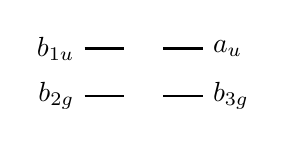
\begin{tikzpicture}[baseline={(current bounding box.center)}]
% lower MOs:
\draw[thick] (0,-0.6) -- (0.5,-0.6)node[pos=0, left] {$b_{2g}$}
;;\draw[thick] (1,-0.6) -- (1.5,-0.6)node[pos=1, right] {$b_{3g}$}
;;
% upper MOs:
\draw[thick] (0,0) -- (0.5,0)node[pos=0, left] {$b_{1u}$}
;;\draw[thick] (1,0) -- (1.5,0)node[pos=1, right] {$a_{u}$}
;;
\end{tikzpicture}$$
In the following, we will leave out the explicit labeling by orbital symmetry. Each monomer will simply be written as:

$$\begin{tikzpicture}[baseline={(current bounding box.center)}]
% lower MOs:
\draw[thick] (0,-0.6) -- (0.5,-0.6)%node[pos=0, left] {$b_{2g}$}
;;\draw[thick] (1,-0.6) -- (1.5,-0.6)%node[pos=1, right] {$b_{3g}$}
;;
% upper MOs:
\draw[thick] (0,0) -- (0.5,0)%node[pos=0, left] {$b_{1u}$}
;;\draw[thick] (1,0) -- (1.5,0)%node[pos=1, right] {$a_{u}$}
;;
\end{tikzpicture}$$
where the character of the orbital is defined by its position. \\ \\ 


Dimer configurations will be written as their monomer occupations, by writing one monomer to the left and one to the right. The orbital ordering within the group of monomer orbitals follows the above mentioned definition. \\ \\ The transformation of monomer orbitals into dimer orbitals is given by knowing the negative and positive linear combinations of monomer orbitals into dimer orbitals. Transforming this known equation system leads to: 
\begin{subequations}\begin{gather*}
a_{u}^{l} = +b_{1g}+a_{u}  \\
b_{1u}^{l} = +a_{g}+b_{1u}  \\
b_{2g}^{l} = +b_{3u}+b_{2g}  \\
b_{3g}^{l} = +b_{2u}+b_{3g}  \\
a_{u}^{r} = -b_{1g}+a_{u}  \\
b_{1u}^{r} = -a_{g}+b_{1u}  \\
b_{2g}^{r} = -b_{3u}+b_{2g}  \\
b_{3g}^{r} = -b_{2u}+b_{3g}
\end{gather*}\end{subequations}
\newpage

\section{Monomer States and Configurations} 
\[S = 
 \quad + \left(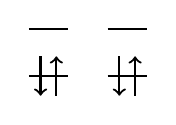
\begin{tikzpicture}[baseline={(current bounding box.center)}]
% lower MOs:
\draw[thick] (0,-0.6) -- (0.5,-0.6)%node[pos=0, left] {$b_{2g}$}
;\draw[->, thick] (0.35, -0.85) -- (0.35, -0.35) ; 
 \draw[<-, thick] (0.15, -0.85) -- (0.15, -0.35) ;\draw[thick] (1,-0.6) -- (1.5,-0.6)%node[pos=1, right] {$b_{3g}$}
;\draw[->, thick] (1.35, -0.85) -- (1.35, -0.35) ; 
 \draw[<-, thick] (1.15, -0.85) -- (1.15, -0.35) ;
% upper MOs:
\draw[thick] (0,0) -- (0.5,0)%node[pos=0, left] {$b_{1u}$}
;;\draw[thick] (1,0) -- (1.5,0)%node[pos=1, right] {$a_{u}$}
;;
\end{tikzpicture}\right) 
 \quad = \left|\underbrace{(b_{1u}^{l})^{0}(b_{2g}^{l})^{2}(b_{3g}^{l})^{2}(a_{u}^{l})^{0}}_{a_{g}}\right|\]
\[Q = 
 \quad + \left(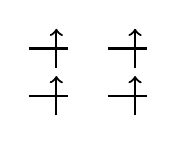
\begin{tikzpicture}[baseline={(current bounding box.center)}]
% lower MOs:
\draw[thick] (0,-0.6) -- (0.5,-0.6)%node[pos=0, left] {$b_{2g}$}
;\draw[->, thick] (0.35, -0.85) -- (0.35, -0.35) ;\draw[thick] (1,-0.6) -- (1.5,-0.6)%node[pos=1, right] {$b_{3g}$}
;\draw[->, thick] (1.35, -0.85) -- (1.35, -0.35) ;
% upper MOs:
\draw[thick] (0,0) -- (0.5,0)%node[pos=0, left] {$b_{1u}$}
;\draw[->, thick] (0.35, -0.25) -- (0.35, 0.25) ;\draw[thick] (1,0) -- (1.5,0)%node[pos=1, right] {$a_{u}$}
;\draw[->, thick] (1.35, -0.25) -- (1.35, 0.25) ;
\end{tikzpicture}\right) 
 \quad = \left|\underbrace{(b_{1u}^{l})^{1}(b_{2g}^{l})^{1}(b_{3g}^{l})^{1}(a_{u}^{l})^{1}}_{a_{g}}\right|\]
\[i^3 b_{2u} = 
 \quad + \left(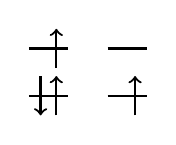
\begin{tikzpicture}[baseline={(current bounding box.center)}]
% lower MOs:
\draw[thick] (0,-0.6) -- (0.5,-0.6)%node[pos=0, left] {$b_{2g}$}
;\draw[->, thick] (0.35, -0.85) -- (0.35, -0.35) ; 
 \draw[<-, thick] (0.15, -0.85) -- (0.15, -0.35) ;\draw[thick] (1,-0.6) -- (1.5,-0.6)%node[pos=1, right] {$b_{3g}$}
;\draw[->, thick] (1.35, -0.85) -- (1.35, -0.35) ;
% upper MOs:
\draw[thick] (0,0) -- (0.5,0)%node[pos=0, left] {$b_{1u}$}
;\draw[->, thick] (0.35, -0.25) -- (0.35, 0.25) ;\draw[thick] (1,0) -- (1.5,0)%node[pos=1, right] {$a_{u}$}
;;
\end{tikzpicture}\right) 
- \left(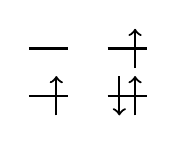
\begin{tikzpicture}[baseline={(current bounding box.center)}]
% lower MOs:
\draw[thick] (0,-0.6) -- (0.5,-0.6)%node[pos=0, left] {$b_{2g}$}
;\draw[->, thick] (0.35, -0.85) -- (0.35, -0.35) ;\draw[thick] (1,-0.6) -- (1.5,-0.6)%node[pos=1, right] {$b_{3g}$}
;\draw[->, thick] (1.35, -0.85) -- (1.35, -0.35) ; 
 \draw[<-, thick] (1.15, -0.85) -- (1.15, -0.35) ;
% upper MOs:
\draw[thick] (0,0) -- (0.5,0)%node[pos=0, left] {$b_{1u}$}
;;\draw[thick] (1,0) -- (1.5,0)%node[pos=1, right] {$a_{u}$}
;\draw[->, thick] (1.35, -0.25) -- (1.35, 0.25) ;
\end{tikzpicture}\right) 
 \quad = \left|\underbrace{(b_{1u}^{l})^{1}(b_{2g}^{l})^{2}(b_{3g}^{l})^{1}(a_{u}^{l})^{0}}_{b_{2u}}\right| - \left|\underbrace{(b_{1u}^{l})^{0}(b_{2g}^{l})^{1}(b_{3g}^{l})^{2}(a_{u}^{l})^{1}}_{b_{2u}}\right|\]
\[e^3 b_{2u} = 
 \quad + \left(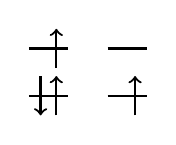
\begin{tikzpicture}[baseline={(current bounding box.center)}]
% lower MOs:
\draw[thick] (0,-0.6) -- (0.5,-0.6)%node[pos=0, left] {$b_{2g}$}
;\draw[->, thick] (0.35, -0.85) -- (0.35, -0.35) ; 
 \draw[<-, thick] (0.15, -0.85) -- (0.15, -0.35) ;\draw[thick] (1,-0.6) -- (1.5,-0.6)%node[pos=1, right] {$b_{3g}$}
;\draw[->, thick] (1.35, -0.85) -- (1.35, -0.35) ;
% upper MOs:
\draw[thick] (0,0) -- (0.5,0)%node[pos=0, left] {$b_{1u}$}
;\draw[->, thick] (0.35, -0.25) -- (0.35, 0.25) ;\draw[thick] (1,0) -- (1.5,0)%node[pos=1, right] {$a_{u}$}
;;
\end{tikzpicture}\right) 
+ \left(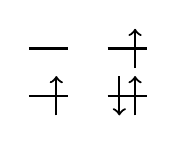
\begin{tikzpicture}[baseline={(current bounding box.center)}]
% lower MOs:
\draw[thick] (0,-0.6) -- (0.5,-0.6)%node[pos=0, left] {$b_{2g}$}
;\draw[->, thick] (0.35, -0.85) -- (0.35, -0.35) ;\draw[thick] (1,-0.6) -- (1.5,-0.6)%node[pos=1, right] {$b_{3g}$}
;\draw[->, thick] (1.35, -0.85) -- (1.35, -0.35) ; 
 \draw[<-, thick] (1.15, -0.85) -- (1.15, -0.35) ;
% upper MOs:
\draw[thick] (0,0) -- (0.5,0)%node[pos=0, left] {$b_{1u}$}
;;\draw[thick] (1,0) -- (1.5,0)%node[pos=1, right] {$a_{u}$}
;\draw[->, thick] (1.35, -0.25) -- (1.35, 0.25) ;
\end{tikzpicture}\right) 
 \quad = \left|\underbrace{(b_{1u}^{l})^{1}(b_{2g}^{l})^{2}(b_{3g}^{l})^{1}(a_{u}^{l})^{0}}_{b_{2u}}\right| + \left|\underbrace{(b_{1u}^{l})^{0}(b_{2g}^{l})^{1}(b_{3g}^{l})^{2}(a_{u}^{l})^{1}}_{b_{2u}}\right|\]
\[e^3 b_{3u} = 
 \quad + \left(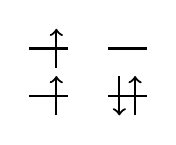
\begin{tikzpicture}[baseline={(current bounding box.center)}]
% lower MOs:
\draw[thick] (0,-0.6) -- (0.5,-0.6)%node[pos=0, left] {$b_{2g}$}
;\draw[->, thick] (0.35, -0.85) -- (0.35, -0.35) ;\draw[thick] (1,-0.6) -- (1.5,-0.6)%node[pos=1, right] {$b_{3g}$}
;\draw[->, thick] (1.35, -0.85) -- (1.35, -0.35) ; 
 \draw[<-, thick] (1.15, -0.85) -- (1.15, -0.35) ;
% upper MOs:
\draw[thick] (0,0) -- (0.5,0)%node[pos=0, left] {$b_{1u}$}
;\draw[->, thick] (0.35, -0.25) -- (0.35, 0.25) ;\draw[thick] (1,0) -- (1.5,0)%node[pos=1, right] {$a_{u}$}
;;
\end{tikzpicture}\right) 
- \left(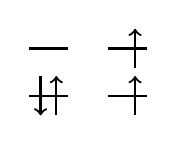
\begin{tikzpicture}[baseline={(current bounding box.center)}]
% lower MOs:
\draw[thick] (0,-0.6) -- (0.5,-0.6)%node[pos=0, left] {$b_{2g}$}
;\draw[->, thick] (0.35, -0.85) -- (0.35, -0.35) ; 
 \draw[<-, thick] (0.15, -0.85) -- (0.15, -0.35) ;\draw[thick] (1,-0.6) -- (1.5,-0.6)%node[pos=1, right] {$b_{3g}$}
;\draw[->, thick] (1.35, -0.85) -- (1.35, -0.35) ;
% upper MOs:
\draw[thick] (0,0) -- (0.5,0)%node[pos=0, left] {$b_{1u}$}
;;\draw[thick] (1,0) -- (1.5,0)%node[pos=1, right] {$a_{u}$}
;\draw[->, thick] (1.35, -0.25) -- (1.35, 0.25) ;
\end{tikzpicture}\right) 
 \quad = \left|\underbrace{(b_{1u}^{l})^{1}(b_{2g}^{l})^{1}(b_{3g}^{l})^{2}(a_{u}^{l})^{0}}_{b_{3u}}\right| - \left|\underbrace{(b_{1u}^{l})^{0}(b_{2g}^{l})^{2}(b_{3g}^{l})^{1}(a_{u}^{l})^{1}}_{b_{3u}}\right|\]
\[i^3 b_{3u} = 
 \quad + \left(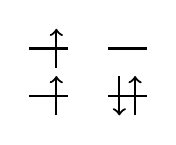
\begin{tikzpicture}[baseline={(current bounding box.center)}]
% lower MOs:
\draw[thick] (0,-0.6) -- (0.5,-0.6)%node[pos=0, left] {$b_{2g}$}
;\draw[->, thick] (0.35, -0.85) -- (0.35, -0.35) ;\draw[thick] (1,-0.6) -- (1.5,-0.6)%node[pos=1, right] {$b_{3g}$}
;\draw[->, thick] (1.35, -0.85) -- (1.35, -0.35) ; 
 \draw[<-, thick] (1.15, -0.85) -- (1.15, -0.35) ;
% upper MOs:
\draw[thick] (0,0) -- (0.5,0)%node[pos=0, left] {$b_{1u}$}
;\draw[->, thick] (0.35, -0.25) -- (0.35, 0.25) ;\draw[thick] (1,0) -- (1.5,0)%node[pos=1, right] {$a_{u}$}
;;
\end{tikzpicture}\right) 
+ \left(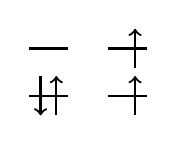
\begin{tikzpicture}[baseline={(current bounding box.center)}]
% lower MOs:
\draw[thick] (0,-0.6) -- (0.5,-0.6)%node[pos=0, left] {$b_{2g}$}
;\draw[->, thick] (0.35, -0.85) -- (0.35, -0.35) ; 
 \draw[<-, thick] (0.15, -0.85) -- (0.15, -0.35) ;\draw[thick] (1,-0.6) -- (1.5,-0.6)%node[pos=1, right] {$b_{3g}$}
;\draw[->, thick] (1.35, -0.85) -- (1.35, -0.35) ;
% upper MOs:
\draw[thick] (0,0) -- (0.5,0)%node[pos=0, left] {$b_{1u}$}
;;\draw[thick] (1,0) -- (1.5,0)%node[pos=1, right] {$a_{u}$}
;\draw[->, thick] (1.35, -0.25) -- (1.35, 0.25) ;
\end{tikzpicture}\right) 
 \quad = \left|\underbrace{(b_{1u}^{l})^{1}(b_{2g}^{l})^{1}(b_{3g}^{l})^{2}(a_{u}^{l})^{0}}_{b_{3u}}\right| + \left|\underbrace{(b_{1u}^{l})^{0}(b_{2g}^{l})^{2}(b_{3g}^{l})^{1}(a_{u}^{l})^{1}}_{b_{3u}}\right|\]
\newpage

\section{Linear Combinations} 

\subsection{\boldmath $S * Q + Q * S$}
\[S * Q + Q * S\]
\[+ \left(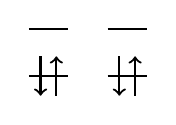
\begin{tikzpicture}[baseline={(current bounding box.center)}]
% lower MOs:
\draw[thick] (0,-0.6) -- (0.5,-0.6)%node[pos=0, left] {$b_{2g}$}
;\draw[->, thick] (0.35, -0.85) -- (0.35, -0.35) ; 
 \draw[<-, thick] (0.15, -0.85) -- (0.15, -0.35) ;\draw[thick] (1,-0.6) -- (1.5,-0.6)%node[pos=1, right] {$b_{3g}$}
;\draw[->, thick] (1.35, -0.85) -- (1.35, -0.35) ; 
 \draw[<-, thick] (1.15, -0.85) -- (1.15, -0.35) ;
% upper MOs:
\draw[thick] (0,0) -- (0.5,0)%node[pos=0, left] {$b_{1u}$}
;;\draw[thick] (1,0) -- (1.5,0)%node[pos=1, right] {$a_{u}$}
;;
\end{tikzpicture}
\quad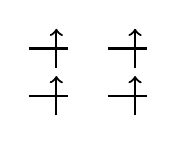
\begin{tikzpicture}[baseline={(current bounding box.center)}]
% lower MOs:
\draw[thick] (0,-0.6) -- (0.5,-0.6)%node[pos=0, left] {$b_{2g}$}
;\draw[->, thick] (0.35, -0.85) -- (0.35, -0.35) ;\draw[thick] (1,-0.6) -- (1.5,-0.6)%node[pos=1, right] {$b_{3g}$}
;\draw[->, thick] (1.35, -0.85) -- (1.35, -0.35) ;
% upper MOs:
\draw[thick] (0,0) -- (0.5,0)%node[pos=0, left] {$b_{1u}$}
;\draw[->, thick] (0.35, -0.25) -- (0.35, 0.25) ;\draw[thick] (1,0) -- (1.5,0)%node[pos=1, right] {$a_{u}$}
;\draw[->, thick] (1.35, -0.25) -- (1.35, 0.25) ;
\end{tikzpicture}\right) 
 + \left(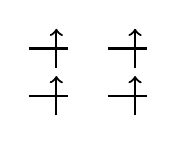
\begin{tikzpicture}[baseline={(current bounding box.center)}]
% lower MOs:
\draw[thick] (0,-0.6) -- (0.5,-0.6)%node[pos=0, left] {$b_{2g}$}
;\draw[->, thick] (0.35, -0.85) -- (0.35, -0.35) ;\draw[thick] (1,-0.6) -- (1.5,-0.6)%node[pos=1, right] {$b_{3g}$}
;\draw[->, thick] (1.35, -0.85) -- (1.35, -0.35) ;
% upper MOs:
\draw[thick] (0,0) -- (0.5,0)%node[pos=0, left] {$b_{1u}$}
;\draw[->, thick] (0.35, -0.25) -- (0.35, 0.25) ;\draw[thick] (1,0) -- (1.5,0)%node[pos=1, right] {$a_{u}$}
;\draw[->, thick] (1.35, -0.25) -- (1.35, 0.25) ;
\end{tikzpicture}
\quad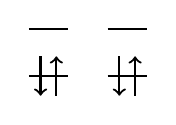
\begin{tikzpicture}[baseline={(current bounding box.center)}]
% lower MOs:
\draw[thick] (0,-0.6) -- (0.5,-0.6)%node[pos=0, left] {$b_{2g}$}
;\draw[->, thick] (0.35, -0.85) -- (0.35, -0.35) ; 
 \draw[<-, thick] (0.15, -0.85) -- (0.15, -0.35) ;\draw[thick] (1,-0.6) -- (1.5,-0.6)%node[pos=1, right] {$b_{3g}$}
;\draw[->, thick] (1.35, -0.85) -- (1.35, -0.35) ; 
 \draw[<-, thick] (1.15, -0.85) -- (1.15, -0.35) ;
% upper MOs:
\draw[thick] (0,0) -- (0.5,0)%node[pos=0, left] {$b_{1u}$}
;;\draw[thick] (1,0) -- (1.5,0)%node[pos=1, right] {$a_{u}$}
;;
\end{tikzpicture}\right) 
\]
monomer ci vectors:
$$\begin{array}{c}
+\left|\underbrace{(b_{1u}^{l})^{0}(b_{2g}^{l})^{2}(b_{3g}^{l})^{2}(a_{u}^{l})^{0}}_{a_{g}^{l}}\right| \cdot{} \left|\underbrace{(b_{1u}^{r})^{1}(b_{2g}^{r})^{1}(b_{3g}^{r})^{1}(a_{u}^{r})^{1}}_{a_{g}^{r}}\right| +\left|\underbrace{(b_{1u}^{l})^{1}(b_{2g}^{l})^{1}(b_{3g}^{l})^{1}(a_{u}^{l})^{1}}_{a_{g}^{l}}\right| \cdot{} \left|\underbrace{(b_{1u}^{r})^{0}(b_{2g}^{r})^{2}(b_{3g}^{r})^{2}(a_{u}^{r})^{0}}_{a_{g}^{r}}\right|
\end{array}$$substitution by dimer orbitals:
$$+\left|\underbrace{(+a_{g}+b_{1u})^{0}(+b_{3u}+b_{2g})^{2}(+b_{2u}+b_{3g})^{2}(+b_{1g}+a_{u})^{0}}_{a_{g}^{l}}\right| \cdot{} \left|\underbrace{(-a_{g}+b_{1u})^{1}(-b_{3u}+b_{2g})^{1}(-b_{2u}+b_{3g})^{1}(-b_{1g}+a_{u})^{1}}_{a_{g}^{r}}\right| + \hdots $$(multiplied out and summed up) dimer ci vectors:

\begin{multline*}\begin{array}{c}
+2 \cdot \left|\underbrace{(a_{g})^{0}(b_{3u})^{2}(b_{2u})^{2}(b_{1g})^{0}(b_{1u})^{1}(b_{2g})^{1}(b_{3g})^{1}(a_{u})^{1}}_{a_{g}}\right| +2 \cdot \left|\underbrace{(a_{g})^{0}(b_{3u})^{2}(b_{2u})^{1}(b_{1g})^{1}(b_{1u})^{1}(b_{2g})^{1}(b_{3g})^{2}(a_{u})^{0}}_{a_{g}}\right| \\[0.5cm] -2 \cdot \left|\underbrace{(a_{g})^{0}(b_{3u})^{1}(b_{2u})^{2}(b_{1g})^{1}(b_{1u})^{1}(b_{2g})^{2}(b_{3g})^{1}(a_{u})^{0}}_{a_{g}}\right| +2 \cdot \left|\underbrace{(a_{g})^{0}(b_{3u})^{1}(b_{2u})^{1}(b_{1g})^{0}(b_{1u})^{1}(b_{2g})^{2}(b_{3g})^{2}(a_{u})^{1}}_{a_{g}}\right| \\[0.5cm] +2 \cdot \left|\underbrace{(a_{g})^{1}(b_{3u})^{2}(b_{2u})^{2}(b_{1g})^{1}(b_{1u})^{0}(b_{2g})^{1}(b_{3g})^{1}(a_{u})^{0}}_{a_{g}}\right| -2 \cdot \left|\underbrace{(a_{g})^{1}(b_{3u})^{2}(b_{2u})^{1}(b_{1g})^{0}(b_{1u})^{0}(b_{2g})^{1}(b_{3g})^{2}(a_{u})^{1}}_{a_{g}}\right| \\[0.5cm] +2 \cdot \left|\underbrace{(a_{g})^{1}(b_{3u})^{1}(b_{2u})^{2}(b_{1g})^{0}(b_{1u})^{0}(b_{2g})^{2}(b_{3g})^{1}(a_{u})^{1}}_{a_{g}}\right| +2 \cdot \left|\underbrace{(a_{g})^{1}(b_{3u})^{1}(b_{2u})^{1}(b_{1g})^{1}(b_{1u})^{0}(b_{2g})^{2}(b_{3g})^{2}(a_{u})^{0}}_{a_{g}}\right|
\end{array}\end{multline*}


\vspace{0.5cm}

\newpage

\subsection{\boldmath $S * Q - Q * S$}
\[S * Q - Q * S\]
\[+ \left(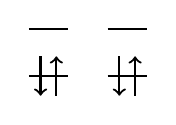
\begin{tikzpicture}[baseline={(current bounding box.center)}]
% lower MOs:
\draw[thick] (0,-0.6) -- (0.5,-0.6)%node[pos=0, left] {$b_{2g}$}
;\draw[->, thick] (0.35, -0.85) -- (0.35, -0.35) ; 
 \draw[<-, thick] (0.15, -0.85) -- (0.15, -0.35) ;\draw[thick] (1,-0.6) -- (1.5,-0.6)%node[pos=1, right] {$b_{3g}$}
;\draw[->, thick] (1.35, -0.85) -- (1.35, -0.35) ; 
 \draw[<-, thick] (1.15, -0.85) -- (1.15, -0.35) ;
% upper MOs:
\draw[thick] (0,0) -- (0.5,0)%node[pos=0, left] {$b_{1u}$}
;;\draw[thick] (1,0) -- (1.5,0)%node[pos=1, right] {$a_{u}$}
;;
\end{tikzpicture}
\quad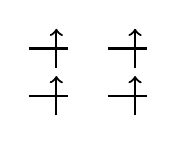
\begin{tikzpicture}[baseline={(current bounding box.center)}]
% lower MOs:
\draw[thick] (0,-0.6) -- (0.5,-0.6)%node[pos=0, left] {$b_{2g}$}
;\draw[->, thick] (0.35, -0.85) -- (0.35, -0.35) ;\draw[thick] (1,-0.6) -- (1.5,-0.6)%node[pos=1, right] {$b_{3g}$}
;\draw[->, thick] (1.35, -0.85) -- (1.35, -0.35) ;
% upper MOs:
\draw[thick] (0,0) -- (0.5,0)%node[pos=0, left] {$b_{1u}$}
;\draw[->, thick] (0.35, -0.25) -- (0.35, 0.25) ;\draw[thick] (1,0) -- (1.5,0)%node[pos=1, right] {$a_{u}$}
;\draw[->, thick] (1.35, -0.25) -- (1.35, 0.25) ;
\end{tikzpicture}\right) 
 - \left(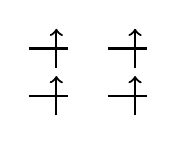
\begin{tikzpicture}[baseline={(current bounding box.center)}]
% lower MOs:
\draw[thick] (0,-0.6) -- (0.5,-0.6)%node[pos=0, left] {$b_{2g}$}
;\draw[->, thick] (0.35, -0.85) -- (0.35, -0.35) ;\draw[thick] (1,-0.6) -- (1.5,-0.6)%node[pos=1, right] {$b_{3g}$}
;\draw[->, thick] (1.35, -0.85) -- (1.35, -0.35) ;
% upper MOs:
\draw[thick] (0,0) -- (0.5,0)%node[pos=0, left] {$b_{1u}$}
;\draw[->, thick] (0.35, -0.25) -- (0.35, 0.25) ;\draw[thick] (1,0) -- (1.5,0)%node[pos=1, right] {$a_{u}$}
;\draw[->, thick] (1.35, -0.25) -- (1.35, 0.25) ;
\end{tikzpicture}
\quad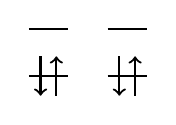
\begin{tikzpicture}[baseline={(current bounding box.center)}]
% lower MOs:
\draw[thick] (0,-0.6) -- (0.5,-0.6)%node[pos=0, left] {$b_{2g}$}
;\draw[->, thick] (0.35, -0.85) -- (0.35, -0.35) ; 
 \draw[<-, thick] (0.15, -0.85) -- (0.15, -0.35) ;\draw[thick] (1,-0.6) -- (1.5,-0.6)%node[pos=1, right] {$b_{3g}$}
;\draw[->, thick] (1.35, -0.85) -- (1.35, -0.35) ; 
 \draw[<-, thick] (1.15, -0.85) -- (1.15, -0.35) ;
% upper MOs:
\draw[thick] (0,0) -- (0.5,0)%node[pos=0, left] {$b_{1u}$}
;;\draw[thick] (1,0) -- (1.5,0)%node[pos=1, right] {$a_{u}$}
;;
\end{tikzpicture}\right) 
\]
monomer ci vectors:
$$\begin{array}{c}
+\left|\underbrace{(b_{1u}^{l})^{0}(b_{2g}^{l})^{2}(b_{3g}^{l})^{2}(a_{u}^{l})^{0}}_{a_{g}^{l}}\right| \cdot{} \left|\underbrace{(b_{1u}^{r})^{1}(b_{2g}^{r})^{1}(b_{3g}^{r})^{1}(a_{u}^{r})^{1}}_{a_{g}^{r}}\right| -\left|\underbrace{(b_{1u}^{l})^{1}(b_{2g}^{l})^{1}(b_{3g}^{l})^{1}(a_{u}^{l})^{1}}_{a_{g}^{l}}\right| \cdot{} \left|\underbrace{(b_{1u}^{r})^{0}(b_{2g}^{r})^{2}(b_{3g}^{r})^{2}(a_{u}^{r})^{0}}_{a_{g}^{r}}\right|
\end{array}$$substitution by dimer orbitals:
$$+\left|\underbrace{(+a_{g}+b_{1u})^{0}(+b_{3u}+b_{2g})^{2}(+b_{2u}+b_{3g})^{2}(+b_{1g}+a_{u})^{0}}_{a_{g}^{l}}\right| \cdot{} \left|\underbrace{(-a_{g}+b_{1u})^{1}(-b_{3u}+b_{2g})^{1}(-b_{2u}+b_{3g})^{1}(-b_{1g}+a_{u})^{1}}_{a_{g}^{r}}\right| + \hdots $$(multiplied out and summed up) dimer ci vectors:

\begin{multline*}\begin{array}{c}
+2 \cdot \left|\underbrace{(a_{g})^{0}(b_{3u})^{2}(b_{2u})^{2}(b_{1g})^{1}(b_{1u})^{1}(b_{2g})^{1}(b_{3g})^{1}(a_{u})^{0}}_{b_{1u}}\right| -2 \cdot \left|\underbrace{(a_{g})^{0}(b_{3u})^{2}(b_{2u})^{1}(b_{1g})^{0}(b_{1u})^{1}(b_{2g})^{1}(b_{3g})^{2}(a_{u})^{1}}_{b_{1u}}\right| \\[0.5cm] +2 \cdot \left|\underbrace{(a_{g})^{0}(b_{3u})^{1}(b_{2u})^{2}(b_{1g})^{0}(b_{1u})^{1}(b_{2g})^{2}(b_{3g})^{1}(a_{u})^{1}}_{b_{1u}}\right| +2 \cdot \left|\underbrace{(a_{g})^{0}(b_{3u})^{1}(b_{2u})^{1}(b_{1g})^{1}(b_{1u})^{1}(b_{2g})^{2}(b_{3g})^{2}(a_{u})^{0}}_{b_{1u}}\right| \\[0.5cm] -2 \cdot \left|\underbrace{(a_{g})^{1}(b_{3u})^{2}(b_{2u})^{2}(b_{1g})^{0}(b_{1u})^{0}(b_{2g})^{1}(b_{3g})^{1}(a_{u})^{1}}_{b_{1u}}\right| -2 \cdot \left|\underbrace{(a_{g})^{1}(b_{3u})^{2}(b_{2u})^{1}(b_{1g})^{1}(b_{1u})^{0}(b_{2g})^{1}(b_{3g})^{2}(a_{u})^{0}}_{b_{1u}}\right| \\[0.5cm] +2 \cdot \left|\underbrace{(a_{g})^{1}(b_{3u})^{1}(b_{2u})^{2}(b_{1g})^{1}(b_{1u})^{0}(b_{2g})^{2}(b_{3g})^{1}(a_{u})^{0}}_{b_{1u}}\right| -2 \cdot \left|\underbrace{(a_{g})^{1}(b_{3u})^{1}(b_{2u})^{1}(b_{1g})^{0}(b_{1u})^{0}(b_{2g})^{2}(b_{3g})^{2}(a_{u})^{1}}_{b_{1u}}\right|
\end{array}\end{multline*}


\vspace{0.5cm}

\newpage

\subsection{\boldmath $i^3 b_{2u} * i^3 b_{2u}$}
\[i^3 b_{2u} * i^3 b_{2u}\]
\[\begin{array}{c}
+ \left(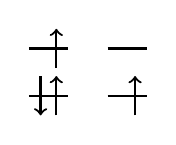
\begin{tikzpicture}[baseline={(current bounding box.center)}]
% lower MOs:
\draw[thick] (0,-0.6) -- (0.5,-0.6)%node[pos=0, left] {$b_{2g}$}
;\draw[->, thick] (0.35, -0.85) -- (0.35, -0.35) ; 
 \draw[<-, thick] (0.15, -0.85) -- (0.15, -0.35) ;\draw[thick] (1,-0.6) -- (1.5,-0.6)%node[pos=1, right] {$b_{3g}$}
;\draw[->, thick] (1.35, -0.85) -- (1.35, -0.35) ;
% upper MOs:
\draw[thick] (0,0) -- (0.5,0)%node[pos=0, left] {$b_{1u}$}
;\draw[->, thick] (0.35, -0.25) -- (0.35, 0.25) ;\draw[thick] (1,0) -- (1.5,0)%node[pos=1, right] {$a_{u}$}
;;
\end{tikzpicture}
\quad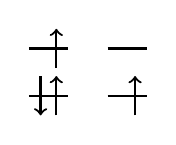
\begin{tikzpicture}[baseline={(current bounding box.center)}]
% lower MOs:
\draw[thick] (0,-0.6) -- (0.5,-0.6)%node[pos=0, left] {$b_{2g}$}
;\draw[->, thick] (0.35, -0.85) -- (0.35, -0.35) ; 
 \draw[<-, thick] (0.15, -0.85) -- (0.15, -0.35) ;\draw[thick] (1,-0.6) -- (1.5,-0.6)%node[pos=1, right] {$b_{3g}$}
;\draw[->, thick] (1.35, -0.85) -- (1.35, -0.35) ;
% upper MOs:
\draw[thick] (0,0) -- (0.5,0)%node[pos=0, left] {$b_{1u}$}
;\draw[->, thick] (0.35, -0.25) -- (0.35, 0.25) ;\draw[thick] (1,0) -- (1.5,0)%node[pos=1, right] {$a_{u}$}
;;
\end{tikzpicture}\right) 
 - \left(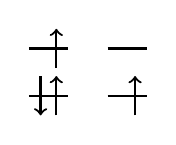
\begin{tikzpicture}[baseline={(current bounding box.center)}]
% lower MOs:
\draw[thick] (0,-0.6) -- (0.5,-0.6)%node[pos=0, left] {$b_{2g}$}
;\draw[->, thick] (0.35, -0.85) -- (0.35, -0.35) ; 
 \draw[<-, thick] (0.15, -0.85) -- (0.15, -0.35) ;\draw[thick] (1,-0.6) -- (1.5,-0.6)%node[pos=1, right] {$b_{3g}$}
;\draw[->, thick] (1.35, -0.85) -- (1.35, -0.35) ;
% upper MOs:
\draw[thick] (0,0) -- (0.5,0)%node[pos=0, left] {$b_{1u}$}
;\draw[->, thick] (0.35, -0.25) -- (0.35, 0.25) ;\draw[thick] (1,0) -- (1.5,0)%node[pos=1, right] {$a_{u}$}
;;
\end{tikzpicture}
\quad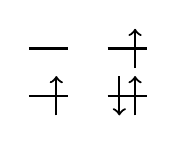
\begin{tikzpicture}[baseline={(current bounding box.center)}]
% lower MOs:
\draw[thick] (0,-0.6) -- (0.5,-0.6)%node[pos=0, left] {$b_{2g}$}
;\draw[->, thick] (0.35, -0.85) -- (0.35, -0.35) ;\draw[thick] (1,-0.6) -- (1.5,-0.6)%node[pos=1, right] {$b_{3g}$}
;\draw[->, thick] (1.35, -0.85) -- (1.35, -0.35) ; 
 \draw[<-, thick] (1.15, -0.85) -- (1.15, -0.35) ;
% upper MOs:
\draw[thick] (0,0) -- (0.5,0)%node[pos=0, left] {$b_{1u}$}
;;\draw[thick] (1,0) -- (1.5,0)%node[pos=1, right] {$a_{u}$}
;\draw[->, thick] (1.35, -0.25) -- (1.35, 0.25) ;
\end{tikzpicture}\right) 
 - \left(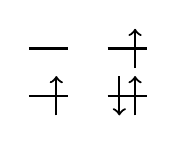
\begin{tikzpicture}[baseline={(current bounding box.center)}]
% lower MOs:
\draw[thick] (0,-0.6) -- (0.5,-0.6)%node[pos=0, left] {$b_{2g}$}
;\draw[->, thick] (0.35, -0.85) -- (0.35, -0.35) ;\draw[thick] (1,-0.6) -- (1.5,-0.6)%node[pos=1, right] {$b_{3g}$}
;\draw[->, thick] (1.35, -0.85) -- (1.35, -0.35) ; 
 \draw[<-, thick] (1.15, -0.85) -- (1.15, -0.35) ;
% upper MOs:
\draw[thick] (0,0) -- (0.5,0)%node[pos=0, left] {$b_{1u}$}
;;\draw[thick] (1,0) -- (1.5,0)%node[pos=1, right] {$a_{u}$}
;\draw[->, thick] (1.35, -0.25) -- (1.35, 0.25) ;
\end{tikzpicture}
\quad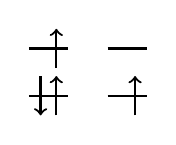
\begin{tikzpicture}[baseline={(current bounding box.center)}]
% lower MOs:
\draw[thick] (0,-0.6) -- (0.5,-0.6)%node[pos=0, left] {$b_{2g}$}
;\draw[->, thick] (0.35, -0.85) -- (0.35, -0.35) ; 
 \draw[<-, thick] (0.15, -0.85) -- (0.15, -0.35) ;\draw[thick] (1,-0.6) -- (1.5,-0.6)%node[pos=1, right] {$b_{3g}$}
;\draw[->, thick] (1.35, -0.85) -- (1.35, -0.35) ;
% upper MOs:
\draw[thick] (0,0) -- (0.5,0)%node[pos=0, left] {$b_{1u}$}
;\draw[->, thick] (0.35, -0.25) -- (0.35, 0.25) ;\draw[thick] (1,0) -- (1.5,0)%node[pos=1, right] {$a_{u}$}
;;
\end{tikzpicture}\right) 
 + \left(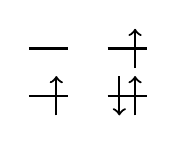
\begin{tikzpicture}[baseline={(current bounding box.center)}]
% lower MOs:
\draw[thick] (0,-0.6) -- (0.5,-0.6)%node[pos=0, left] {$b_{2g}$}
;\draw[->, thick] (0.35, -0.85) -- (0.35, -0.35) ;\draw[thick] (1,-0.6) -- (1.5,-0.6)%node[pos=1, right] {$b_{3g}$}
;\draw[->, thick] (1.35, -0.85) -- (1.35, -0.35) ; 
 \draw[<-, thick] (1.15, -0.85) -- (1.15, -0.35) ;
% upper MOs:
\draw[thick] (0,0) -- (0.5,0)%node[pos=0, left] {$b_{1u}$}
;;\draw[thick] (1,0) -- (1.5,0)%node[pos=1, right] {$a_{u}$}
;\draw[->, thick] (1.35, -0.25) -- (1.35, 0.25) ;
\end{tikzpicture}
\quad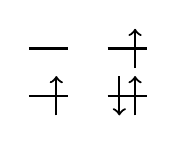
\begin{tikzpicture}[baseline={(current bounding box.center)}]
% lower MOs:
\draw[thick] (0,-0.6) -- (0.5,-0.6)%node[pos=0, left] {$b_{2g}$}
;\draw[->, thick] (0.35, -0.85) -- (0.35, -0.35) ;\draw[thick] (1,-0.6) -- (1.5,-0.6)%node[pos=1, right] {$b_{3g}$}
;\draw[->, thick] (1.35, -0.85) -- (1.35, -0.35) ; 
 \draw[<-, thick] (1.15, -0.85) -- (1.15, -0.35) ;
% upper MOs:
\draw[thick] (0,0) -- (0.5,0)%node[pos=0, left] {$b_{1u}$}
;;\draw[thick] (1,0) -- (1.5,0)%node[pos=1, right] {$a_{u}$}
;\draw[->, thick] (1.35, -0.25) -- (1.35, 0.25) ;
\end{tikzpicture}\right) 

\end{array}\]
monomer ci vectors:
$$\begin{array}{c}
+\left|\underbrace{(b_{1u}^{l})^{1}(b_{2g}^{l})^{2}(b_{3g}^{l})^{1}(a_{u}^{l})^{0}}_{b_{2u}^{l}}\right| \cdot{} \left|\underbrace{(b_{1u}^{r})^{1}(b_{2g}^{r})^{2}(b_{3g}^{r})^{1}(a_{u}^{r})^{0}}_{b_{2u}^{r}}\right| -\left|\underbrace{(b_{1u}^{l})^{1}(b_{2g}^{l})^{2}(b_{3g}^{l})^{1}(a_{u}^{l})^{0}}_{b_{2u}^{l}}\right| \cdot{} \left|\underbrace{(b_{1u}^{r})^{0}(b_{2g}^{r})^{1}(b_{3g}^{r})^{2}(a_{u}^{r})^{1}}_{b_{2u}^{r}}\right| \\[0.5cm] -\left|\underbrace{(b_{1u}^{l})^{0}(b_{2g}^{l})^{1}(b_{3g}^{l})^{2}(a_{u}^{l})^{1}}_{b_{2u}^{l}}\right| \cdot{} \left|\underbrace{(b_{1u}^{r})^{1}(b_{2g}^{r})^{2}(b_{3g}^{r})^{1}(a_{u}^{r})^{0}}_{b_{2u}^{r}}\right| +\left|\underbrace{(b_{1u}^{l})^{0}(b_{2g}^{l})^{1}(b_{3g}^{l})^{2}(a_{u}^{l})^{1}}_{b_{2u}^{l}}\right| \cdot{} \left|\underbrace{(b_{1u}^{r})^{0}(b_{2g}^{r})^{1}(b_{3g}^{r})^{2}(a_{u}^{r})^{1}}_{b_{2u}^{r}}\right|
\end{array}$$substitution by dimer orbitals:
$$+\left|\underbrace{(+a_{g}+b_{1u})^{1}(+b_{3u}+b_{2g})^{2}(+b_{2u}+b_{3g})^{1}(+b_{1g}+a_{u})^{0}}_{b_{2u}^{l}}\right| \cdot{} \left|\underbrace{(-a_{g}+b_{1u})^{1}(-b_{3u}+b_{2g})^{2}(-b_{2u}+b_{3g})^{1}(-b_{1g}+a_{u})^{0}}_{b_{2u}^{r}}\right| + \hdots $$(multiplied out and summed up) dimer ci vectors:

\begin{multline*}\begin{array}{c}
+\left|\underbrace{(a_{g})^{1}(b_{3u})^{2}(b_{2u})^{1}(b_{1g})^{0}(b_{1u})^{1}(b_{2g})^{2}(b_{3g})^{1}(a_{u})^{0}}_{a_{g}}\right| -2 \cdot \left|\underbrace{(a_{g})^{1}(b_{3u})^{2}(b_{2u})^{1}(b_{1g})^{0}(b_{1u})^{0}(b_{2g})^{1}(b_{3g})^{2}(a_{u})^{1}}_{a_{g}}\right| \\[0.5cm] -2 \cdot \left|\underbrace{(a_{g})^{1}(b_{3u})^{2}(b_{2u})^{2}(b_{1g})^{1}(b_{1u})^{0}(b_{2g})^{1}(b_{3g})^{1}(a_{u})^{0}}_{a_{g}}\right| +2 \cdot \left|\underbrace{(a_{g})^{1}(b_{3u})^{1}(b_{2u})^{1}(b_{1g})^{1}(b_{1u})^{0}(b_{2g})^{2}(b_{3g})^{2}(a_{u})^{0}}_{a_{g}}\right| \\[0.5cm] -2 \cdot \left|\underbrace{(a_{g})^{1}(b_{3u})^{1}(b_{2u})^{2}(b_{1g})^{0}(b_{1u})^{0}(b_{2g})^{2}(b_{3g})^{1}(a_{u})^{1}}_{a_{g}}\right| -2 \cdot \left|\underbrace{(a_{g})^{0}(b_{3u})^{2}(b_{2u})^{1}(b_{1g})^{1}(b_{1u})^{1}(b_{2g})^{1}(b_{3g})^{2}(a_{u})^{0}}_{a_{g}}\right| \\[0.5cm] +2 \cdot \left|\underbrace{(a_{g})^{0}(b_{3u})^{2}(b_{2u})^{2}(b_{1g})^{0}(b_{1u})^{1}(b_{2g})^{1}(b_{3g})^{1}(a_{u})^{1}}_{a_{g}}\right| -2 \cdot \left|\underbrace{(a_{g})^{0}(b_{3u})^{1}(b_{2u})^{1}(b_{1g})^{0}(b_{1u})^{1}(b_{2g})^{2}(b_{3g})^{2}(a_{u})^{1}}_{a_{g}}\right| \\[0.5cm] -2 \cdot \left|\underbrace{(a_{g})^{0}(b_{3u})^{1}(b_{2u})^{2}(b_{1g})^{1}(b_{1u})^{1}(b_{2g})^{2}(b_{3g})^{1}(a_{u})^{0}}_{a_{g}}\right| +\left|\underbrace{(a_{g})^{0}(b_{3u})^{1}(b_{2u})^{2}(b_{1g})^{1}(b_{1u})^{0}(b_{2g})^{1}(b_{3g})^{2}(a_{u})^{1}}_{a_{g}}\right|
\end{array}\end{multline*}


\vspace{0.5cm}

\newpage

\subsection{\boldmath $i^3 b_{2u} * e^3 b_{2u} + e^3 b_{2u} * i^3 b_{2u}$}
\[i^3 b_{2u} * e^3 b_{2u} + e^3 b_{2u} * i^3 b_{2u}\]
\[\begin{array}{c}
+ \left(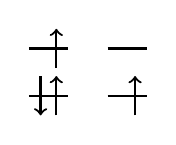
\begin{tikzpicture}[baseline={(current bounding box.center)}]
% lower MOs:
\draw[thick] (0,-0.6) -- (0.5,-0.6)%node[pos=0, left] {$b_{2g}$}
;\draw[->, thick] (0.35, -0.85) -- (0.35, -0.35) ; 
 \draw[<-, thick] (0.15, -0.85) -- (0.15, -0.35) ;\draw[thick] (1,-0.6) -- (1.5,-0.6)%node[pos=1, right] {$b_{3g}$}
;\draw[->, thick] (1.35, -0.85) -- (1.35, -0.35) ;
% upper MOs:
\draw[thick] (0,0) -- (0.5,0)%node[pos=0, left] {$b_{1u}$}
;\draw[->, thick] (0.35, -0.25) -- (0.35, 0.25) ;\draw[thick] (1,0) -- (1.5,0)%node[pos=1, right] {$a_{u}$}
;;
\end{tikzpicture}
\quad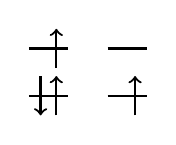
\begin{tikzpicture}[baseline={(current bounding box.center)}]
% lower MOs:
\draw[thick] (0,-0.6) -- (0.5,-0.6)%node[pos=0, left] {$b_{2g}$}
;\draw[->, thick] (0.35, -0.85) -- (0.35, -0.35) ; 
 \draw[<-, thick] (0.15, -0.85) -- (0.15, -0.35) ;\draw[thick] (1,-0.6) -- (1.5,-0.6)%node[pos=1, right] {$b_{3g}$}
;\draw[->, thick] (1.35, -0.85) -- (1.35, -0.35) ;
% upper MOs:
\draw[thick] (0,0) -- (0.5,0)%node[pos=0, left] {$b_{1u}$}
;\draw[->, thick] (0.35, -0.25) -- (0.35, 0.25) ;\draw[thick] (1,0) -- (1.5,0)%node[pos=1, right] {$a_{u}$}
;;
\end{tikzpicture}\right) 
 + \left(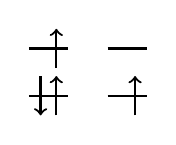
\begin{tikzpicture}[baseline={(current bounding box.center)}]
% lower MOs:
\draw[thick] (0,-0.6) -- (0.5,-0.6)%node[pos=0, left] {$b_{2g}$}
;\draw[->, thick] (0.35, -0.85) -- (0.35, -0.35) ; 
 \draw[<-, thick] (0.15, -0.85) -- (0.15, -0.35) ;\draw[thick] (1,-0.6) -- (1.5,-0.6)%node[pos=1, right] {$b_{3g}$}
;\draw[->, thick] (1.35, -0.85) -- (1.35, -0.35) ;
% upper MOs:
\draw[thick] (0,0) -- (0.5,0)%node[pos=0, left] {$b_{1u}$}
;\draw[->, thick] (0.35, -0.25) -- (0.35, 0.25) ;\draw[thick] (1,0) -- (1.5,0)%node[pos=1, right] {$a_{u}$}
;;
\end{tikzpicture}
\quad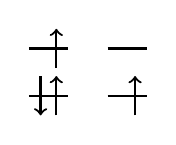
\begin{tikzpicture}[baseline={(current bounding box.center)}]
% lower MOs:
\draw[thick] (0,-0.6) -- (0.5,-0.6)%node[pos=0, left] {$b_{2g}$}
;\draw[->, thick] (0.35, -0.85) -- (0.35, -0.35) ; 
 \draw[<-, thick] (0.15, -0.85) -- (0.15, -0.35) ;\draw[thick] (1,-0.6) -- (1.5,-0.6)%node[pos=1, right] {$b_{3g}$}
;\draw[->, thick] (1.35, -0.85) -- (1.35, -0.35) ;
% upper MOs:
\draw[thick] (0,0) -- (0.5,0)%node[pos=0, left] {$b_{1u}$}
;\draw[->, thick] (0.35, -0.25) -- (0.35, 0.25) ;\draw[thick] (1,0) -- (1.5,0)%node[pos=1, right] {$a_{u}$}
;;
\end{tikzpicture}\right) 
 + \left(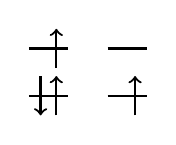
\begin{tikzpicture}[baseline={(current bounding box.center)}]
% lower MOs:
\draw[thick] (0,-0.6) -- (0.5,-0.6)%node[pos=0, left] {$b_{2g}$}
;\draw[->, thick] (0.35, -0.85) -- (0.35, -0.35) ; 
 \draw[<-, thick] (0.15, -0.85) -- (0.15, -0.35) ;\draw[thick] (1,-0.6) -- (1.5,-0.6)%node[pos=1, right] {$b_{3g}$}
;\draw[->, thick] (1.35, -0.85) -- (1.35, -0.35) ;
% upper MOs:
\draw[thick] (0,0) -- (0.5,0)%node[pos=0, left] {$b_{1u}$}
;\draw[->, thick] (0.35, -0.25) -- (0.35, 0.25) ;\draw[thick] (1,0) -- (1.5,0)%node[pos=1, right] {$a_{u}$}
;;
\end{tikzpicture}
\quad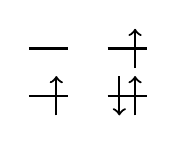
\begin{tikzpicture}[baseline={(current bounding box.center)}]
% lower MOs:
\draw[thick] (0,-0.6) -- (0.5,-0.6)%node[pos=0, left] {$b_{2g}$}
;\draw[->, thick] (0.35, -0.85) -- (0.35, -0.35) ;\draw[thick] (1,-0.6) -- (1.5,-0.6)%node[pos=1, right] {$b_{3g}$}
;\draw[->, thick] (1.35, -0.85) -- (1.35, -0.35) ; 
 \draw[<-, thick] (1.15, -0.85) -- (1.15, -0.35) ;
% upper MOs:
\draw[thick] (0,0) -- (0.5,0)%node[pos=0, left] {$b_{1u}$}
;;\draw[thick] (1,0) -- (1.5,0)%node[pos=1, right] {$a_{u}$}
;\draw[->, thick] (1.35, -0.25) -- (1.35, 0.25) ;
\end{tikzpicture}\right) 
 + \left(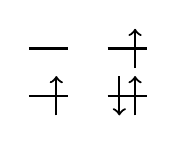
\begin{tikzpicture}[baseline={(current bounding box.center)}]
% lower MOs:
\draw[thick] (0,-0.6) -- (0.5,-0.6)%node[pos=0, left] {$b_{2g}$}
;\draw[->, thick] (0.35, -0.85) -- (0.35, -0.35) ;\draw[thick] (1,-0.6) -- (1.5,-0.6)%node[pos=1, right] {$b_{3g}$}
;\draw[->, thick] (1.35, -0.85) -- (1.35, -0.35) ; 
 \draw[<-, thick] (1.15, -0.85) -- (1.15, -0.35) ;
% upper MOs:
\draw[thick] (0,0) -- (0.5,0)%node[pos=0, left] {$b_{1u}$}
;;\draw[thick] (1,0) -- (1.5,0)%node[pos=1, right] {$a_{u}$}
;\draw[->, thick] (1.35, -0.25) -- (1.35, 0.25) ;
\end{tikzpicture}
\quad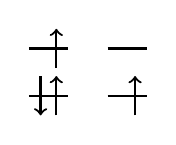
\begin{tikzpicture}[baseline={(current bounding box.center)}]
% lower MOs:
\draw[thick] (0,-0.6) -- (0.5,-0.6)%node[pos=0, left] {$b_{2g}$}
;\draw[->, thick] (0.35, -0.85) -- (0.35, -0.35) ; 
 \draw[<-, thick] (0.15, -0.85) -- (0.15, -0.35) ;\draw[thick] (1,-0.6) -- (1.5,-0.6)%node[pos=1, right] {$b_{3g}$}
;\draw[->, thick] (1.35, -0.85) -- (1.35, -0.35) ;
% upper MOs:
\draw[thick] (0,0) -- (0.5,0)%node[pos=0, left] {$b_{1u}$}
;\draw[->, thick] (0.35, -0.25) -- (0.35, 0.25) ;\draw[thick] (1,0) -- (1.5,0)%node[pos=1, right] {$a_{u}$}
;;
\end{tikzpicture}\right) 
 \\[0.5cm] - \left(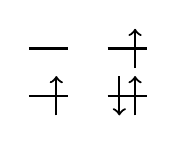
\begin{tikzpicture}[baseline={(current bounding box.center)}]
% lower MOs:
\draw[thick] (0,-0.6) -- (0.5,-0.6)%node[pos=0, left] {$b_{2g}$}
;\draw[->, thick] (0.35, -0.85) -- (0.35, -0.35) ;\draw[thick] (1,-0.6) -- (1.5,-0.6)%node[pos=1, right] {$b_{3g}$}
;\draw[->, thick] (1.35, -0.85) -- (1.35, -0.35) ; 
 \draw[<-, thick] (1.15, -0.85) -- (1.15, -0.35) ;
% upper MOs:
\draw[thick] (0,0) -- (0.5,0)%node[pos=0, left] {$b_{1u}$}
;;\draw[thick] (1,0) -- (1.5,0)%node[pos=1, right] {$a_{u}$}
;\draw[->, thick] (1.35, -0.25) -- (1.35, 0.25) ;
\end{tikzpicture}
\quad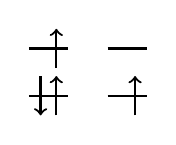
\begin{tikzpicture}[baseline={(current bounding box.center)}]
% lower MOs:
\draw[thick] (0,-0.6) -- (0.5,-0.6)%node[pos=0, left] {$b_{2g}$}
;\draw[->, thick] (0.35, -0.85) -- (0.35, -0.35) ; 
 \draw[<-, thick] (0.15, -0.85) -- (0.15, -0.35) ;\draw[thick] (1,-0.6) -- (1.5,-0.6)%node[pos=1, right] {$b_{3g}$}
;\draw[->, thick] (1.35, -0.85) -- (1.35, -0.35) ;
% upper MOs:
\draw[thick] (0,0) -- (0.5,0)%node[pos=0, left] {$b_{1u}$}
;\draw[->, thick] (0.35, -0.25) -- (0.35, 0.25) ;\draw[thick] (1,0) -- (1.5,0)%node[pos=1, right] {$a_{u}$}
;;
\end{tikzpicture}\right) 
 - \left(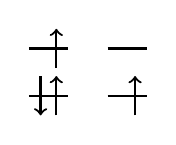
\begin{tikzpicture}[baseline={(current bounding box.center)}]
% lower MOs:
\draw[thick] (0,-0.6) -- (0.5,-0.6)%node[pos=0, left] {$b_{2g}$}
;\draw[->, thick] (0.35, -0.85) -- (0.35, -0.35) ; 
 \draw[<-, thick] (0.15, -0.85) -- (0.15, -0.35) ;\draw[thick] (1,-0.6) -- (1.5,-0.6)%node[pos=1, right] {$b_{3g}$}
;\draw[->, thick] (1.35, -0.85) -- (1.35, -0.35) ;
% upper MOs:
\draw[thick] (0,0) -- (0.5,0)%node[pos=0, left] {$b_{1u}$}
;\draw[->, thick] (0.35, -0.25) -- (0.35, 0.25) ;\draw[thick] (1,0) -- (1.5,0)%node[pos=1, right] {$a_{u}$}
;;
\end{tikzpicture}
\quad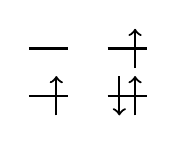
\begin{tikzpicture}[baseline={(current bounding box.center)}]
% lower MOs:
\draw[thick] (0,-0.6) -- (0.5,-0.6)%node[pos=0, left] {$b_{2g}$}
;\draw[->, thick] (0.35, -0.85) -- (0.35, -0.35) ;\draw[thick] (1,-0.6) -- (1.5,-0.6)%node[pos=1, right] {$b_{3g}$}
;\draw[->, thick] (1.35, -0.85) -- (1.35, -0.35) ; 
 \draw[<-, thick] (1.15, -0.85) -- (1.15, -0.35) ;
% upper MOs:
\draw[thick] (0,0) -- (0.5,0)%node[pos=0, left] {$b_{1u}$}
;;\draw[thick] (1,0) -- (1.5,0)%node[pos=1, right] {$a_{u}$}
;\draw[->, thick] (1.35, -0.25) -- (1.35, 0.25) ;
\end{tikzpicture}\right) 
 - \left(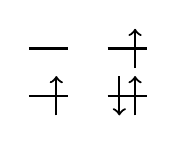
\begin{tikzpicture}[baseline={(current bounding box.center)}]
% lower MOs:
\draw[thick] (0,-0.6) -- (0.5,-0.6)%node[pos=0, left] {$b_{2g}$}
;\draw[->, thick] (0.35, -0.85) -- (0.35, -0.35) ;\draw[thick] (1,-0.6) -- (1.5,-0.6)%node[pos=1, right] {$b_{3g}$}
;\draw[->, thick] (1.35, -0.85) -- (1.35, -0.35) ; 
 \draw[<-, thick] (1.15, -0.85) -- (1.15, -0.35) ;
% upper MOs:
\draw[thick] (0,0) -- (0.5,0)%node[pos=0, left] {$b_{1u}$}
;;\draw[thick] (1,0) -- (1.5,0)%node[pos=1, right] {$a_{u}$}
;\draw[->, thick] (1.35, -0.25) -- (1.35, 0.25) ;
\end{tikzpicture}
\quad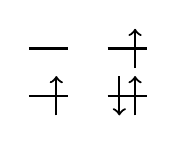
\begin{tikzpicture}[baseline={(current bounding box.center)}]
% lower MOs:
\draw[thick] (0,-0.6) -- (0.5,-0.6)%node[pos=0, left] {$b_{2g}$}
;\draw[->, thick] (0.35, -0.85) -- (0.35, -0.35) ;\draw[thick] (1,-0.6) -- (1.5,-0.6)%node[pos=1, right] {$b_{3g}$}
;\draw[->, thick] (1.35, -0.85) -- (1.35, -0.35) ; 
 \draw[<-, thick] (1.15, -0.85) -- (1.15, -0.35) ;
% upper MOs:
\draw[thick] (0,0) -- (0.5,0)%node[pos=0, left] {$b_{1u}$}
;;\draw[thick] (1,0) -- (1.5,0)%node[pos=1, right] {$a_{u}$}
;\draw[->, thick] (1.35, -0.25) -- (1.35, 0.25) ;
\end{tikzpicture}\right) 
 - \left(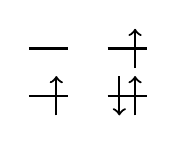
\begin{tikzpicture}[baseline={(current bounding box.center)}]
% lower MOs:
\draw[thick] (0,-0.6) -- (0.5,-0.6)%node[pos=0, left] {$b_{2g}$}
;\draw[->, thick] (0.35, -0.85) -- (0.35, -0.35) ;\draw[thick] (1,-0.6) -- (1.5,-0.6)%node[pos=1, right] {$b_{3g}$}
;\draw[->, thick] (1.35, -0.85) -- (1.35, -0.35) ; 
 \draw[<-, thick] (1.15, -0.85) -- (1.15, -0.35) ;
% upper MOs:
\draw[thick] (0,0) -- (0.5,0)%node[pos=0, left] {$b_{1u}$}
;;\draw[thick] (1,0) -- (1.5,0)%node[pos=1, right] {$a_{u}$}
;\draw[->, thick] (1.35, -0.25) -- (1.35, 0.25) ;
\end{tikzpicture}
\quad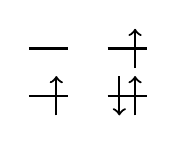
\begin{tikzpicture}[baseline={(current bounding box.center)}]
% lower MOs:
\draw[thick] (0,-0.6) -- (0.5,-0.6)%node[pos=0, left] {$b_{2g}$}
;\draw[->, thick] (0.35, -0.85) -- (0.35, -0.35) ;\draw[thick] (1,-0.6) -- (1.5,-0.6)%node[pos=1, right] {$b_{3g}$}
;\draw[->, thick] (1.35, -0.85) -- (1.35, -0.35) ; 
 \draw[<-, thick] (1.15, -0.85) -- (1.15, -0.35) ;
% upper MOs:
\draw[thick] (0,0) -- (0.5,0)%node[pos=0, left] {$b_{1u}$}
;;\draw[thick] (1,0) -- (1.5,0)%node[pos=1, right] {$a_{u}$}
;\draw[->, thick] (1.35, -0.25) -- (1.35, 0.25) ;
\end{tikzpicture}\right) 

\end{array}\]
monomer ci vectors:
$$\begin{array}{c}
+\left|\underbrace{(b_{1u}^{l})^{1}(b_{2g}^{l})^{2}(b_{3g}^{l})^{1}(a_{u}^{l})^{0}}_{b_{2u}^{l}}\right| \cdot{} \left|\underbrace{(b_{1u}^{r})^{1}(b_{2g}^{r})^{2}(b_{3g}^{r})^{1}(a_{u}^{r})^{0}}_{b_{2u}^{r}}\right| +\left|\underbrace{(b_{1u}^{l})^{1}(b_{2g}^{l})^{2}(b_{3g}^{l})^{1}(a_{u}^{l})^{0}}_{b_{2u}^{l}}\right| \cdot{} \left|\underbrace{(b_{1u}^{r})^{1}(b_{2g}^{r})^{2}(b_{3g}^{r})^{1}(a_{u}^{r})^{0}}_{b_{2u}^{r}}\right| \\[0.5cm] +\left|\underbrace{(b_{1u}^{l})^{1}(b_{2g}^{l})^{2}(b_{3g}^{l})^{1}(a_{u}^{l})^{0}}_{b_{2u}^{l}}\right| \cdot{} \left|\underbrace{(b_{1u}^{r})^{0}(b_{2g}^{r})^{1}(b_{3g}^{r})^{2}(a_{u}^{r})^{1}}_{b_{2u}^{r}}\right| +\left|\underbrace{(b_{1u}^{l})^{0}(b_{2g}^{l})^{1}(b_{3g}^{l})^{2}(a_{u}^{l})^{1}}_{b_{2u}^{l}}\right| \cdot{} \left|\underbrace{(b_{1u}^{r})^{1}(b_{2g}^{r})^{2}(b_{3g}^{r})^{1}(a_{u}^{r})^{0}}_{b_{2u}^{r}}\right| \\[0.5cm] -\left|\underbrace{(b_{1u}^{l})^{0}(b_{2g}^{l})^{1}(b_{3g}^{l})^{2}(a_{u}^{l})^{1}}_{b_{2u}^{l}}\right| \cdot{} \left|\underbrace{(b_{1u}^{r})^{1}(b_{2g}^{r})^{2}(b_{3g}^{r})^{1}(a_{u}^{r})^{0}}_{b_{2u}^{r}}\right| -\left|\underbrace{(b_{1u}^{l})^{1}(b_{2g}^{l})^{2}(b_{3g}^{l})^{1}(a_{u}^{l})^{0}}_{b_{2u}^{l}}\right| \cdot{} \left|\underbrace{(b_{1u}^{r})^{0}(b_{2g}^{r})^{1}(b_{3g}^{r})^{2}(a_{u}^{r})^{1}}_{b_{2u}^{r}}\right| \\[0.5cm] -\left|\underbrace{(b_{1u}^{l})^{0}(b_{2g}^{l})^{1}(b_{3g}^{l})^{2}(a_{u}^{l})^{1}}_{b_{2u}^{l}}\right| \cdot{} \left|\underbrace{(b_{1u}^{r})^{0}(b_{2g}^{r})^{1}(b_{3g}^{r})^{2}(a_{u}^{r})^{1}}_{b_{2u}^{r}}\right| -\left|\underbrace{(b_{1u}^{l})^{0}(b_{2g}^{l})^{1}(b_{3g}^{l})^{2}(a_{u}^{l})^{1}}_{b_{2u}^{l}}\right| \cdot{} \left|\underbrace{(b_{1u}^{r})^{0}(b_{2g}^{r})^{1}(b_{3g}^{r})^{2}(a_{u}^{r})^{1}}_{b_{2u}^{r}}\right|
\end{array}$$substitution by dimer orbitals:
$$+\left|\underbrace{(+a_{g}+b_{1u})^{1}(+b_{3u}+b_{2g})^{2}(+b_{2u}+b_{3g})^{1}(+b_{1g}+a_{u})^{0}}_{b_{2u}^{l}}\right| \cdot{} \left|\underbrace{(-a_{g}+b_{1u})^{1}(-b_{3u}+b_{2g})^{2}(-b_{2u}+b_{3g})^{1}(-b_{1g}+a_{u})^{0}}_{b_{2u}^{r}}\right| + \hdots $$(multiplied out and summed up) dimer ci vectors:

\begin{multline*}\begin{array}{c}
+2 \cdot \left|\underbrace{(a_{g})^{1}(b_{3u})^{2}(b_{2u})^{1}(b_{1g})^{0}(b_{1u})^{1}(b_{2g})^{2}(b_{3g})^{1}(a_{u})^{0}}_{a_{g}}\right| -2 \cdot \left|\underbrace{(a_{g})^{0}(b_{3u})^{1}(b_{2u})^{2}(b_{1g})^{1}(b_{1u})^{0}(b_{2g})^{1}(b_{3g})^{2}(a_{u})^{1}}_{a_{g}}\right|
\end{array}\end{multline*}


\vspace{0.5cm}

\newpage

\subsection{\boldmath $i^3 b_{2u} * e^3 b_{2u} - e^3 b_{2u} * i^3 b_{2u}$}
\[i^3 b_{2u} * e^3 b_{2u} - e^3 b_{2u} * i^3 b_{2u}\]
\[\begin{array}{c}
+ \left(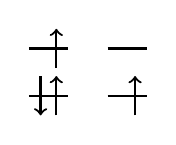
\begin{tikzpicture}[baseline={(current bounding box.center)}]
% lower MOs:
\draw[thick] (0,-0.6) -- (0.5,-0.6)%node[pos=0, left] {$b_{2g}$}
;\draw[->, thick] (0.35, -0.85) -- (0.35, -0.35) ; 
 \draw[<-, thick] (0.15, -0.85) -- (0.15, -0.35) ;\draw[thick] (1,-0.6) -- (1.5,-0.6)%node[pos=1, right] {$b_{3g}$}
;\draw[->, thick] (1.35, -0.85) -- (1.35, -0.35) ;
% upper MOs:
\draw[thick] (0,0) -- (0.5,0)%node[pos=0, left] {$b_{1u}$}
;\draw[->, thick] (0.35, -0.25) -- (0.35, 0.25) ;\draw[thick] (1,0) -- (1.5,0)%node[pos=1, right] {$a_{u}$}
;;
\end{tikzpicture}
\quad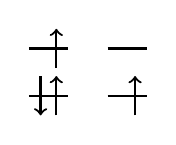
\begin{tikzpicture}[baseline={(current bounding box.center)}]
% lower MOs:
\draw[thick] (0,-0.6) -- (0.5,-0.6)%node[pos=0, left] {$b_{2g}$}
;\draw[->, thick] (0.35, -0.85) -- (0.35, -0.35) ; 
 \draw[<-, thick] (0.15, -0.85) -- (0.15, -0.35) ;\draw[thick] (1,-0.6) -- (1.5,-0.6)%node[pos=1, right] {$b_{3g}$}
;\draw[->, thick] (1.35, -0.85) -- (1.35, -0.35) ;
% upper MOs:
\draw[thick] (0,0) -- (0.5,0)%node[pos=0, left] {$b_{1u}$}
;\draw[->, thick] (0.35, -0.25) -- (0.35, 0.25) ;\draw[thick] (1,0) -- (1.5,0)%node[pos=1, right] {$a_{u}$}
;;
\end{tikzpicture}\right) 
 - \left(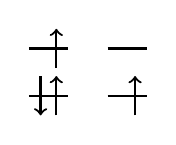
\begin{tikzpicture}[baseline={(current bounding box.center)}]
% lower MOs:
\draw[thick] (0,-0.6) -- (0.5,-0.6)%node[pos=0, left] {$b_{2g}$}
;\draw[->, thick] (0.35, -0.85) -- (0.35, -0.35) ; 
 \draw[<-, thick] (0.15, -0.85) -- (0.15, -0.35) ;\draw[thick] (1,-0.6) -- (1.5,-0.6)%node[pos=1, right] {$b_{3g}$}
;\draw[->, thick] (1.35, -0.85) -- (1.35, -0.35) ;
% upper MOs:
\draw[thick] (0,0) -- (0.5,0)%node[pos=0, left] {$b_{1u}$}
;\draw[->, thick] (0.35, -0.25) -- (0.35, 0.25) ;\draw[thick] (1,0) -- (1.5,0)%node[pos=1, right] {$a_{u}$}
;;
\end{tikzpicture}
\quad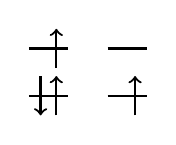
\begin{tikzpicture}[baseline={(current bounding box.center)}]
% lower MOs:
\draw[thick] (0,-0.6) -- (0.5,-0.6)%node[pos=0, left] {$b_{2g}$}
;\draw[->, thick] (0.35, -0.85) -- (0.35, -0.35) ; 
 \draw[<-, thick] (0.15, -0.85) -- (0.15, -0.35) ;\draw[thick] (1,-0.6) -- (1.5,-0.6)%node[pos=1, right] {$b_{3g}$}
;\draw[->, thick] (1.35, -0.85) -- (1.35, -0.35) ;
% upper MOs:
\draw[thick] (0,0) -- (0.5,0)%node[pos=0, left] {$b_{1u}$}
;\draw[->, thick] (0.35, -0.25) -- (0.35, 0.25) ;\draw[thick] (1,0) -- (1.5,0)%node[pos=1, right] {$a_{u}$}
;;
\end{tikzpicture}\right) 
 + \left(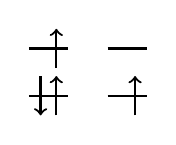
\begin{tikzpicture}[baseline={(current bounding box.center)}]
% lower MOs:
\draw[thick] (0,-0.6) -- (0.5,-0.6)%node[pos=0, left] {$b_{2g}$}
;\draw[->, thick] (0.35, -0.85) -- (0.35, -0.35) ; 
 \draw[<-, thick] (0.15, -0.85) -- (0.15, -0.35) ;\draw[thick] (1,-0.6) -- (1.5,-0.6)%node[pos=1, right] {$b_{3g}$}
;\draw[->, thick] (1.35, -0.85) -- (1.35, -0.35) ;
% upper MOs:
\draw[thick] (0,0) -- (0.5,0)%node[pos=0, left] {$b_{1u}$}
;\draw[->, thick] (0.35, -0.25) -- (0.35, 0.25) ;\draw[thick] (1,0) -- (1.5,0)%node[pos=1, right] {$a_{u}$}
;;
\end{tikzpicture}
\quad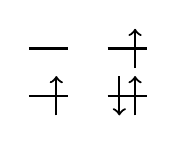
\begin{tikzpicture}[baseline={(current bounding box.center)}]
% lower MOs:
\draw[thick] (0,-0.6) -- (0.5,-0.6)%node[pos=0, left] {$b_{2g}$}
;\draw[->, thick] (0.35, -0.85) -- (0.35, -0.35) ;\draw[thick] (1,-0.6) -- (1.5,-0.6)%node[pos=1, right] {$b_{3g}$}
;\draw[->, thick] (1.35, -0.85) -- (1.35, -0.35) ; 
 \draw[<-, thick] (1.15, -0.85) -- (1.15, -0.35) ;
% upper MOs:
\draw[thick] (0,0) -- (0.5,0)%node[pos=0, left] {$b_{1u}$}
;;\draw[thick] (1,0) -- (1.5,0)%node[pos=1, right] {$a_{u}$}
;\draw[->, thick] (1.35, -0.25) -- (1.35, 0.25) ;
\end{tikzpicture}\right) 
 - \left(\begin{tikzpicture}[baseline={(current bounding box.center)}]
% lower MOs:
\draw[thick] (0,-0.6) -- (0.5,-0.6)%node[pos=0, left] {$b_{2g}$}
;\draw[->, thick] (0.35, -0.85) -- (0.35, -0.35) ;\draw[thick] (1,-0.6) -- (1.5,-0.6)%node[pos=1, right] {$b_{3g}$}
;\draw[->, thick] (1.35, -0.85) -- (1.35, -0.35) ; 
 \draw[<-, thick] (1.15, -0.85) -- (1.15, -0.35) ;
% upper MOs:
\draw[thick] (0,0) -- (0.5,0)%node[pos=0, left] {$b_{1u}$}
;;\draw[thick] (1,0) -- (1.5,0)%node[pos=1, right] {$a_{u}$}
;\draw[->, thick] (1.35, -0.25) -- (1.35, 0.25) ;
\end{tikzpicture}
\quad\begin{tikzpicture}[baseline={(current bounding box.center)}]
% lower MOs:
\draw[thick] (0,-0.6) -- (0.5,-0.6)%node[pos=0, left] {$b_{2g}$}
;\draw[->, thick] (0.35, -0.85) -- (0.35, -0.35) ; 
 \draw[<-, thick] (0.15, -0.85) -- (0.15, -0.35) ;\draw[thick] (1,-0.6) -- (1.5,-0.6)%node[pos=1, right] {$b_{3g}$}
;\draw[->, thick] (1.35, -0.85) -- (1.35, -0.35) ;
% upper MOs:
\draw[thick] (0,0) -- (0.5,0)%node[pos=0, left] {$b_{1u}$}
;\draw[->, thick] (0.35, -0.25) -- (0.35, 0.25) ;\draw[thick] (1,0) -- (1.5,0)%node[pos=1, right] {$a_{u}$}
;;
\end{tikzpicture}\right) 
 \\[0.5cm] - \left(\begin{tikzpicture}[baseline={(current bounding box.center)}]
% lower MOs:
\draw[thick] (0,-0.6) -- (0.5,-0.6)%node[pos=0, left] {$b_{2g}$}
;\draw[->, thick] (0.35, -0.85) -- (0.35, -0.35) ;\draw[thick] (1,-0.6) -- (1.5,-0.6)%node[pos=1, right] {$b_{3g}$}
;\draw[->, thick] (1.35, -0.85) -- (1.35, -0.35) ; 
 \draw[<-, thick] (1.15, -0.85) -- (1.15, -0.35) ;
% upper MOs:
\draw[thick] (0,0) -- (0.5,0)%node[pos=0, left] {$b_{1u}$}
;;\draw[thick] (1,0) -- (1.5,0)%node[pos=1, right] {$a_{u}$}
;\draw[->, thick] (1.35, -0.25) -- (1.35, 0.25) ;
\end{tikzpicture}
\quad\begin{tikzpicture}[baseline={(current bounding box.center)}]
% lower MOs:
\draw[thick] (0,-0.6) -- (0.5,-0.6)%node[pos=0, left] {$b_{2g}$}
;\draw[->, thick] (0.35, -0.85) -- (0.35, -0.35) ; 
 \draw[<-, thick] (0.15, -0.85) -- (0.15, -0.35) ;\draw[thick] (1,-0.6) -- (1.5,-0.6)%node[pos=1, right] {$b_{3g}$}
;\draw[->, thick] (1.35, -0.85) -- (1.35, -0.35) ;
% upper MOs:
\draw[thick] (0,0) -- (0.5,0)%node[pos=0, left] {$b_{1u}$}
;\draw[->, thick] (0.35, -0.25) -- (0.35, 0.25) ;\draw[thick] (1,0) -- (1.5,0)%node[pos=1, right] {$a_{u}$}
;;
\end{tikzpicture}\right) 
 + \left(\begin{tikzpicture}[baseline={(current bounding box.center)}]
% lower MOs:
\draw[thick] (0,-0.6) -- (0.5,-0.6)%node[pos=0, left] {$b_{2g}$}
;\draw[->, thick] (0.35, -0.85) -- (0.35, -0.35) ; 
 \draw[<-, thick] (0.15, -0.85) -- (0.15, -0.35) ;\draw[thick] (1,-0.6) -- (1.5,-0.6)%node[pos=1, right] {$b_{3g}$}
;\draw[->, thick] (1.35, -0.85) -- (1.35, -0.35) ;
% upper MOs:
\draw[thick] (0,0) -- (0.5,0)%node[pos=0, left] {$b_{1u}$}
;\draw[->, thick] (0.35, -0.25) -- (0.35, 0.25) ;\draw[thick] (1,0) -- (1.5,0)%node[pos=1, right] {$a_{u}$}
;;
\end{tikzpicture}
\quad\begin{tikzpicture}[baseline={(current bounding box.center)}]
% lower MOs:
\draw[thick] (0,-0.6) -- (0.5,-0.6)%node[pos=0, left] {$b_{2g}$}
;\draw[->, thick] (0.35, -0.85) -- (0.35, -0.35) ;\draw[thick] (1,-0.6) -- (1.5,-0.6)%node[pos=1, right] {$b_{3g}$}
;\draw[->, thick] (1.35, -0.85) -- (1.35, -0.35) ; 
 \draw[<-, thick] (1.15, -0.85) -- (1.15, -0.35) ;
% upper MOs:
\draw[thick] (0,0) -- (0.5,0)%node[pos=0, left] {$b_{1u}$}
;;\draw[thick] (1,0) -- (1.5,0)%node[pos=1, right] {$a_{u}$}
;\draw[->, thick] (1.35, -0.25) -- (1.35, 0.25) ;
\end{tikzpicture}\right) 
 - \left(\begin{tikzpicture}[baseline={(current bounding box.center)}]
% lower MOs:
\draw[thick] (0,-0.6) -- (0.5,-0.6)%node[pos=0, left] {$b_{2g}$}
;\draw[->, thick] (0.35, -0.85) -- (0.35, -0.35) ;\draw[thick] (1,-0.6) -- (1.5,-0.6)%node[pos=1, right] {$b_{3g}$}
;\draw[->, thick] (1.35, -0.85) -- (1.35, -0.35) ; 
 \draw[<-, thick] (1.15, -0.85) -- (1.15, -0.35) ;
% upper MOs:
\draw[thick] (0,0) -- (0.5,0)%node[pos=0, left] {$b_{1u}$}
;;\draw[thick] (1,0) -- (1.5,0)%node[pos=1, right] {$a_{u}$}
;\draw[->, thick] (1.35, -0.25) -- (1.35, 0.25) ;
\end{tikzpicture}
\quad\begin{tikzpicture}[baseline={(current bounding box.center)}]
% lower MOs:
\draw[thick] (0,-0.6) -- (0.5,-0.6)%node[pos=0, left] {$b_{2g}$}
;\draw[->, thick] (0.35, -0.85) -- (0.35, -0.35) ;\draw[thick] (1,-0.6) -- (1.5,-0.6)%node[pos=1, right] {$b_{3g}$}
;\draw[->, thick] (1.35, -0.85) -- (1.35, -0.35) ; 
 \draw[<-, thick] (1.15, -0.85) -- (1.15, -0.35) ;
% upper MOs:
\draw[thick] (0,0) -- (0.5,0)%node[pos=0, left] {$b_{1u}$}
;;\draw[thick] (1,0) -- (1.5,0)%node[pos=1, right] {$a_{u}$}
;\draw[->, thick] (1.35, -0.25) -- (1.35, 0.25) ;
\end{tikzpicture}\right) 
 + \left(\begin{tikzpicture}[baseline={(current bounding box.center)}]
% lower MOs:
\draw[thick] (0,-0.6) -- (0.5,-0.6)%node[pos=0, left] {$b_{2g}$}
;\draw[->, thick] (0.35, -0.85) -- (0.35, -0.35) ;\draw[thick] (1,-0.6) -- (1.5,-0.6)%node[pos=1, right] {$b_{3g}$}
;\draw[->, thick] (1.35, -0.85) -- (1.35, -0.35) ; 
 \draw[<-, thick] (1.15, -0.85) -- (1.15, -0.35) ;
% upper MOs:
\draw[thick] (0,0) -- (0.5,0)%node[pos=0, left] {$b_{1u}$}
;;\draw[thick] (1,0) -- (1.5,0)%node[pos=1, right] {$a_{u}$}
;\draw[->, thick] (1.35, -0.25) -- (1.35, 0.25) ;
\end{tikzpicture}
\quad\begin{tikzpicture}[baseline={(current bounding box.center)}]
% lower MOs:
\draw[thick] (0,-0.6) -- (0.5,-0.6)%node[pos=0, left] {$b_{2g}$}
;\draw[->, thick] (0.35, -0.85) -- (0.35, -0.35) ;\draw[thick] (1,-0.6) -- (1.5,-0.6)%node[pos=1, right] {$b_{3g}$}
;\draw[->, thick] (1.35, -0.85) -- (1.35, -0.35) ; 
 \draw[<-, thick] (1.15, -0.85) -- (1.15, -0.35) ;
% upper MOs:
\draw[thick] (0,0) -- (0.5,0)%node[pos=0, left] {$b_{1u}$}
;;\draw[thick] (1,0) -- (1.5,0)%node[pos=1, right] {$a_{u}$}
;\draw[->, thick] (1.35, -0.25) -- (1.35, 0.25) ;
\end{tikzpicture}\right) 

\end{array}\]
monomer ci vectors:
$$\begin{array}{c}
+\left|\underbrace{(b_{1u}^{l})^{1}(b_{2g}^{l})^{2}(b_{3g}^{l})^{1}(a_{u}^{l})^{0}}_{b_{2u}^{l}}\right| \cdot{} \left|\underbrace{(b_{1u}^{r})^{1}(b_{2g}^{r})^{2}(b_{3g}^{r})^{1}(a_{u}^{r})^{0}}_{b_{2u}^{r}}\right| -\left|\underbrace{(b_{1u}^{l})^{1}(b_{2g}^{l})^{2}(b_{3g}^{l})^{1}(a_{u}^{l})^{0}}_{b_{2u}^{l}}\right| \cdot{} \left|\underbrace{(b_{1u}^{r})^{1}(b_{2g}^{r})^{2}(b_{3g}^{r})^{1}(a_{u}^{r})^{0}}_{b_{2u}^{r}}\right| \\[0.5cm] +\left|\underbrace{(b_{1u}^{l})^{1}(b_{2g}^{l})^{2}(b_{3g}^{l})^{1}(a_{u}^{l})^{0}}_{b_{2u}^{l}}\right| \cdot{} \left|\underbrace{(b_{1u}^{r})^{0}(b_{2g}^{r})^{1}(b_{3g}^{r})^{2}(a_{u}^{r})^{1}}_{b_{2u}^{r}}\right| -\left|\underbrace{(b_{1u}^{l})^{0}(b_{2g}^{l})^{1}(b_{3g}^{l})^{2}(a_{u}^{l})^{1}}_{b_{2u}^{l}}\right| \cdot{} \left|\underbrace{(b_{1u}^{r})^{1}(b_{2g}^{r})^{2}(b_{3g}^{r})^{1}(a_{u}^{r})^{0}}_{b_{2u}^{r}}\right| \\[0.5cm] -\left|\underbrace{(b_{1u}^{l})^{0}(b_{2g}^{l})^{1}(b_{3g}^{l})^{2}(a_{u}^{l})^{1}}_{b_{2u}^{l}}\right| \cdot{} \left|\underbrace{(b_{1u}^{r})^{1}(b_{2g}^{r})^{2}(b_{3g}^{r})^{1}(a_{u}^{r})^{0}}_{b_{2u}^{r}}\right| +\left|\underbrace{(b_{1u}^{l})^{1}(b_{2g}^{l})^{2}(b_{3g}^{l})^{1}(a_{u}^{l})^{0}}_{b_{2u}^{l}}\right| \cdot{} \left|\underbrace{(b_{1u}^{r})^{0}(b_{2g}^{r})^{1}(b_{3g}^{r})^{2}(a_{u}^{r})^{1}}_{b_{2u}^{r}}\right| \\[0.5cm] -\left|\underbrace{(b_{1u}^{l})^{0}(b_{2g}^{l})^{1}(b_{3g}^{l})^{2}(a_{u}^{l})^{1}}_{b_{2u}^{l}}\right| \cdot{} \left|\underbrace{(b_{1u}^{r})^{0}(b_{2g}^{r})^{1}(b_{3g}^{r})^{2}(a_{u}^{r})^{1}}_{b_{2u}^{r}}\right| +\left|\underbrace{(b_{1u}^{l})^{0}(b_{2g}^{l})^{1}(b_{3g}^{l})^{2}(a_{u}^{l})^{1}}_{b_{2u}^{l}}\right| \cdot{} \left|\underbrace{(b_{1u}^{r})^{0}(b_{2g}^{r})^{1}(b_{3g}^{r})^{2}(a_{u}^{r})^{1}}_{b_{2u}^{r}}\right|
\end{array}$$substitution by dimer orbitals:
$$+\left|\underbrace{(+a_{g}+b_{1u})^{1}(+b_{3u}+b_{2g})^{2}(+b_{2u}+b_{3g})^{1}(+b_{1g}+a_{u})^{0}}_{b_{2u}^{l}}\right| \cdot{} \left|\underbrace{(-a_{g}+b_{1u})^{1}(-b_{3u}+b_{2g})^{2}(-b_{2u}+b_{3g})^{1}(-b_{1g}+a_{u})^{0}}_{b_{2u}^{r}}\right| + \hdots $$(multiplied out and summed up) dimer ci vectors:

\begin{multline*}\begin{array}{c}
+4 \cdot \left|\underbrace{(a_{g})^{1}(b_{3u})^{2}(b_{2u})^{1}(b_{1g})^{1}(b_{1u})^{0}(b_{2g})^{1}(b_{3g})^{2}(a_{u})^{0}}_{b_{1u}}\right| -4 \cdot \left|\underbrace{(a_{g})^{1}(b_{3u})^{2}(b_{2u})^{2}(b_{1g})^{0}(b_{1u})^{0}(b_{2g})^{1}(b_{3g})^{1}(a_{u})^{1}}_{b_{1u}}\right| \\[0.5cm] +4 \cdot \left|\underbrace{(a_{g})^{1}(b_{3u})^{1}(b_{2u})^{1}(b_{1g})^{0}(b_{1u})^{0}(b_{2g})^{2}(b_{3g})^{2}(a_{u})^{1}}_{b_{1u}}\right| +4 \cdot \left|\underbrace{(a_{g})^{1}(b_{3u})^{1}(b_{2u})^{2}(b_{1g})^{1}(b_{1u})^{0}(b_{2g})^{2}(b_{3g})^{1}(a_{u})^{0}}_{b_{1u}}\right| \\[0.5cm] -4 \cdot \left|\underbrace{(a_{g})^{0}(b_{3u})^{2}(b_{2u})^{1}(b_{1g})^{0}(b_{1u})^{1}(b_{2g})^{1}(b_{3g})^{2}(a_{u})^{1}}_{b_{1u}}\right| -4 \cdot \left|\underbrace{(a_{g})^{0}(b_{3u})^{2}(b_{2u})^{2}(b_{1g})^{1}(b_{1u})^{1}(b_{2g})^{1}(b_{3g})^{1}(a_{u})^{0}}_{b_{1u}}\right| \\[0.5cm] +4 \cdot \left|\underbrace{(a_{g})^{0}(b_{3u})^{1}(b_{2u})^{1}(b_{1g})^{1}(b_{1u})^{1}(b_{2g})^{2}(b_{3g})^{2}(a_{u})^{0}}_{b_{1u}}\right| -4 \cdot \left|\underbrace{(a_{g})^{0}(b_{3u})^{1}(b_{2u})^{2}(b_{1g})^{0}(b_{1u})^{1}(b_{2g})^{2}(b_{3g})^{1}(a_{u})^{1}}_{b_{1u}}\right|
\end{array}\end{multline*}


\vspace{0.5cm}

\newpage

\subsection{\boldmath $i^3 b_{2u} * e^3 b_{3u} + e^3 b_{3u} * i^3 b_{2u}$}
\[i^3 b_{2u} * e^3 b_{3u} + e^3 b_{3u} * i^3 b_{2u}\]
\[\begin{array}{c}
+ \left(\begin{tikzpicture}[baseline={(current bounding box.center)}]
% lower MOs:
\draw[thick] (0,-0.6) -- (0.5,-0.6)%node[pos=0, left] {$b_{2g}$}
;\draw[->, thick] (0.35, -0.85) -- (0.35, -0.35) ; 
 \draw[<-, thick] (0.15, -0.85) -- (0.15, -0.35) ;\draw[thick] (1,-0.6) -- (1.5,-0.6)%node[pos=1, right] {$b_{3g}$}
;\draw[->, thick] (1.35, -0.85) -- (1.35, -0.35) ;
% upper MOs:
\draw[thick] (0,0) -- (0.5,0)%node[pos=0, left] {$b_{1u}$}
;\draw[->, thick] (0.35, -0.25) -- (0.35, 0.25) ;\draw[thick] (1,0) -- (1.5,0)%node[pos=1, right] {$a_{u}$}
;;
\end{tikzpicture}
\quad\begin{tikzpicture}[baseline={(current bounding box.center)}]
% lower MOs:
\draw[thick] (0,-0.6) -- (0.5,-0.6)%node[pos=0, left] {$b_{2g}$}
;\draw[->, thick] (0.35, -0.85) -- (0.35, -0.35) ;\draw[thick] (1,-0.6) -- (1.5,-0.6)%node[pos=1, right] {$b_{3g}$}
;\draw[->, thick] (1.35, -0.85) -- (1.35, -0.35) ; 
 \draw[<-, thick] (1.15, -0.85) -- (1.15, -0.35) ;
% upper MOs:
\draw[thick] (0,0) -- (0.5,0)%node[pos=0, left] {$b_{1u}$}
;\draw[->, thick] (0.35, -0.25) -- (0.35, 0.25) ;\draw[thick] (1,0) -- (1.5,0)%node[pos=1, right] {$a_{u}$}
;;
\end{tikzpicture}\right) 
 + \left(\begin{tikzpicture}[baseline={(current bounding box.center)}]
% lower MOs:
\draw[thick] (0,-0.6) -- (0.5,-0.6)%node[pos=0, left] {$b_{2g}$}
;\draw[->, thick] (0.35, -0.85) -- (0.35, -0.35) ;\draw[thick] (1,-0.6) -- (1.5,-0.6)%node[pos=1, right] {$b_{3g}$}
;\draw[->, thick] (1.35, -0.85) -- (1.35, -0.35) ; 
 \draw[<-, thick] (1.15, -0.85) -- (1.15, -0.35) ;
% upper MOs:
\draw[thick] (0,0) -- (0.5,0)%node[pos=0, left] {$b_{1u}$}
;\draw[->, thick] (0.35, -0.25) -- (0.35, 0.25) ;\draw[thick] (1,0) -- (1.5,0)%node[pos=1, right] {$a_{u}$}
;;
\end{tikzpicture}
\quad\begin{tikzpicture}[baseline={(current bounding box.center)}]
% lower MOs:
\draw[thick] (0,-0.6) -- (0.5,-0.6)%node[pos=0, left] {$b_{2g}$}
;\draw[->, thick] (0.35, -0.85) -- (0.35, -0.35) ; 
 \draw[<-, thick] (0.15, -0.85) -- (0.15, -0.35) ;\draw[thick] (1,-0.6) -- (1.5,-0.6)%node[pos=1, right] {$b_{3g}$}
;\draw[->, thick] (1.35, -0.85) -- (1.35, -0.35) ;
% upper MOs:
\draw[thick] (0,0) -- (0.5,0)%node[pos=0, left] {$b_{1u}$}
;\draw[->, thick] (0.35, -0.25) -- (0.35, 0.25) ;\draw[thick] (1,0) -- (1.5,0)%node[pos=1, right] {$a_{u}$}
;;
\end{tikzpicture}\right) 
 - \left(\begin{tikzpicture}[baseline={(current bounding box.center)}]
% lower MOs:
\draw[thick] (0,-0.6) -- (0.5,-0.6)%node[pos=0, left] {$b_{2g}$}
;\draw[->, thick] (0.35, -0.85) -- (0.35, -0.35) ; 
 \draw[<-, thick] (0.15, -0.85) -- (0.15, -0.35) ;\draw[thick] (1,-0.6) -- (1.5,-0.6)%node[pos=1, right] {$b_{3g}$}
;\draw[->, thick] (1.35, -0.85) -- (1.35, -0.35) ;
% upper MOs:
\draw[thick] (0,0) -- (0.5,0)%node[pos=0, left] {$b_{1u}$}
;\draw[->, thick] (0.35, -0.25) -- (0.35, 0.25) ;\draw[thick] (1,0) -- (1.5,0)%node[pos=1, right] {$a_{u}$}
;;
\end{tikzpicture}
\quad\begin{tikzpicture}[baseline={(current bounding box.center)}]
% lower MOs:
\draw[thick] (0,-0.6) -- (0.5,-0.6)%node[pos=0, left] {$b_{2g}$}
;\draw[->, thick] (0.35, -0.85) -- (0.35, -0.35) ; 
 \draw[<-, thick] (0.15, -0.85) -- (0.15, -0.35) ;\draw[thick] (1,-0.6) -- (1.5,-0.6)%node[pos=1, right] {$b_{3g}$}
;\draw[->, thick] (1.35, -0.85) -- (1.35, -0.35) ;
% upper MOs:
\draw[thick] (0,0) -- (0.5,0)%node[pos=0, left] {$b_{1u}$}
;;\draw[thick] (1,0) -- (1.5,0)%node[pos=1, right] {$a_{u}$}
;\draw[->, thick] (1.35, -0.25) -- (1.35, 0.25) ;
\end{tikzpicture}\right) 
 - \left(\begin{tikzpicture}[baseline={(current bounding box.center)}]
% lower MOs:
\draw[thick] (0,-0.6) -- (0.5,-0.6)%node[pos=0, left] {$b_{2g}$}
;\draw[->, thick] (0.35, -0.85) -- (0.35, -0.35) ; 
 \draw[<-, thick] (0.15, -0.85) -- (0.15, -0.35) ;\draw[thick] (1,-0.6) -- (1.5,-0.6)%node[pos=1, right] {$b_{3g}$}
;\draw[->, thick] (1.35, -0.85) -- (1.35, -0.35) ;
% upper MOs:
\draw[thick] (0,0) -- (0.5,0)%node[pos=0, left] {$b_{1u}$}
;;\draw[thick] (1,0) -- (1.5,0)%node[pos=1, right] {$a_{u}$}
;\draw[->, thick] (1.35, -0.25) -- (1.35, 0.25) ;
\end{tikzpicture}
\quad\begin{tikzpicture}[baseline={(current bounding box.center)}]
% lower MOs:
\draw[thick] (0,-0.6) -- (0.5,-0.6)%node[pos=0, left] {$b_{2g}$}
;\draw[->, thick] (0.35, -0.85) -- (0.35, -0.35) ; 
 \draw[<-, thick] (0.15, -0.85) -- (0.15, -0.35) ;\draw[thick] (1,-0.6) -- (1.5,-0.6)%node[pos=1, right] {$b_{3g}$}
;\draw[->, thick] (1.35, -0.85) -- (1.35, -0.35) ;
% upper MOs:
\draw[thick] (0,0) -- (0.5,0)%node[pos=0, left] {$b_{1u}$}
;\draw[->, thick] (0.35, -0.25) -- (0.35, 0.25) ;\draw[thick] (1,0) -- (1.5,0)%node[pos=1, right] {$a_{u}$}
;;
\end{tikzpicture}\right) 
 \\[0.5cm] - \left(\begin{tikzpicture}[baseline={(current bounding box.center)}]
% lower MOs:
\draw[thick] (0,-0.6) -- (0.5,-0.6)%node[pos=0, left] {$b_{2g}$}
;\draw[->, thick] (0.35, -0.85) -- (0.35, -0.35) ;\draw[thick] (1,-0.6) -- (1.5,-0.6)%node[pos=1, right] {$b_{3g}$}
;\draw[->, thick] (1.35, -0.85) -- (1.35, -0.35) ; 
 \draw[<-, thick] (1.15, -0.85) -- (1.15, -0.35) ;
% upper MOs:
\draw[thick] (0,0) -- (0.5,0)%node[pos=0, left] {$b_{1u}$}
;;\draw[thick] (1,0) -- (1.5,0)%node[pos=1, right] {$a_{u}$}
;\draw[->, thick] (1.35, -0.25) -- (1.35, 0.25) ;
\end{tikzpicture}
\quad\begin{tikzpicture}[baseline={(current bounding box.center)}]
% lower MOs:
\draw[thick] (0,-0.6) -- (0.5,-0.6)%node[pos=0, left] {$b_{2g}$}
;\draw[->, thick] (0.35, -0.85) -- (0.35, -0.35) ;\draw[thick] (1,-0.6) -- (1.5,-0.6)%node[pos=1, right] {$b_{3g}$}
;\draw[->, thick] (1.35, -0.85) -- (1.35, -0.35) ; 
 \draw[<-, thick] (1.15, -0.85) -- (1.15, -0.35) ;
% upper MOs:
\draw[thick] (0,0) -- (0.5,0)%node[pos=0, left] {$b_{1u}$}
;\draw[->, thick] (0.35, -0.25) -- (0.35, 0.25) ;\draw[thick] (1,0) -- (1.5,0)%node[pos=1, right] {$a_{u}$}
;;
\end{tikzpicture}\right) 
 - \left(\begin{tikzpicture}[baseline={(current bounding box.center)}]
% lower MOs:
\draw[thick] (0,-0.6) -- (0.5,-0.6)%node[pos=0, left] {$b_{2g}$}
;\draw[->, thick] (0.35, -0.85) -- (0.35, -0.35) ;\draw[thick] (1,-0.6) -- (1.5,-0.6)%node[pos=1, right] {$b_{3g}$}
;\draw[->, thick] (1.35, -0.85) -- (1.35, -0.35) ; 
 \draw[<-, thick] (1.15, -0.85) -- (1.15, -0.35) ;
% upper MOs:
\draw[thick] (0,0) -- (0.5,0)%node[pos=0, left] {$b_{1u}$}
;\draw[->, thick] (0.35, -0.25) -- (0.35, 0.25) ;\draw[thick] (1,0) -- (1.5,0)%node[pos=1, right] {$a_{u}$}
;;
\end{tikzpicture}
\quad\begin{tikzpicture}[baseline={(current bounding box.center)}]
% lower MOs:
\draw[thick] (0,-0.6) -- (0.5,-0.6)%node[pos=0, left] {$b_{2g}$}
;\draw[->, thick] (0.35, -0.85) -- (0.35, -0.35) ;\draw[thick] (1,-0.6) -- (1.5,-0.6)%node[pos=1, right] {$b_{3g}$}
;\draw[->, thick] (1.35, -0.85) -- (1.35, -0.35) ; 
 \draw[<-, thick] (1.15, -0.85) -- (1.15, -0.35) ;
% upper MOs:
\draw[thick] (0,0) -- (0.5,0)%node[pos=0, left] {$b_{1u}$}
;;\draw[thick] (1,0) -- (1.5,0)%node[pos=1, right] {$a_{u}$}
;\draw[->, thick] (1.35, -0.25) -- (1.35, 0.25) ;
\end{tikzpicture}\right) 
 + \left(\begin{tikzpicture}[baseline={(current bounding box.center)}]
% lower MOs:
\draw[thick] (0,-0.6) -- (0.5,-0.6)%node[pos=0, left] {$b_{2g}$}
;\draw[->, thick] (0.35, -0.85) -- (0.35, -0.35) ;\draw[thick] (1,-0.6) -- (1.5,-0.6)%node[pos=1, right] {$b_{3g}$}
;\draw[->, thick] (1.35, -0.85) -- (1.35, -0.35) ; 
 \draw[<-, thick] (1.15, -0.85) -- (1.15, -0.35) ;
% upper MOs:
\draw[thick] (0,0) -- (0.5,0)%node[pos=0, left] {$b_{1u}$}
;;\draw[thick] (1,0) -- (1.5,0)%node[pos=1, right] {$a_{u}$}
;\draw[->, thick] (1.35, -0.25) -- (1.35, 0.25) ;
\end{tikzpicture}
\quad\begin{tikzpicture}[baseline={(current bounding box.center)}]
% lower MOs:
\draw[thick] (0,-0.6) -- (0.5,-0.6)%node[pos=0, left] {$b_{2g}$}
;\draw[->, thick] (0.35, -0.85) -- (0.35, -0.35) ; 
 \draw[<-, thick] (0.15, -0.85) -- (0.15, -0.35) ;\draw[thick] (1,-0.6) -- (1.5,-0.6)%node[pos=1, right] {$b_{3g}$}
;\draw[->, thick] (1.35, -0.85) -- (1.35, -0.35) ;
% upper MOs:
\draw[thick] (0,0) -- (0.5,0)%node[pos=0, left] {$b_{1u}$}
;;\draw[thick] (1,0) -- (1.5,0)%node[pos=1, right] {$a_{u}$}
;\draw[->, thick] (1.35, -0.25) -- (1.35, 0.25) ;
\end{tikzpicture}\right) 
 + \left(\begin{tikzpicture}[baseline={(current bounding box.center)}]
% lower MOs:
\draw[thick] (0,-0.6) -- (0.5,-0.6)%node[pos=0, left] {$b_{2g}$}
;\draw[->, thick] (0.35, -0.85) -- (0.35, -0.35) ; 
 \draw[<-, thick] (0.15, -0.85) -- (0.15, -0.35) ;\draw[thick] (1,-0.6) -- (1.5,-0.6)%node[pos=1, right] {$b_{3g}$}
;\draw[->, thick] (1.35, -0.85) -- (1.35, -0.35) ;
% upper MOs:
\draw[thick] (0,0) -- (0.5,0)%node[pos=0, left] {$b_{1u}$}
;;\draw[thick] (1,0) -- (1.5,0)%node[pos=1, right] {$a_{u}$}
;\draw[->, thick] (1.35, -0.25) -- (1.35, 0.25) ;
\end{tikzpicture}
\quad\begin{tikzpicture}[baseline={(current bounding box.center)}]
% lower MOs:
\draw[thick] (0,-0.6) -- (0.5,-0.6)%node[pos=0, left] {$b_{2g}$}
;\draw[->, thick] (0.35, -0.85) -- (0.35, -0.35) ;\draw[thick] (1,-0.6) -- (1.5,-0.6)%node[pos=1, right] {$b_{3g}$}
;\draw[->, thick] (1.35, -0.85) -- (1.35, -0.35) ; 
 \draw[<-, thick] (1.15, -0.85) -- (1.15, -0.35) ;
% upper MOs:
\draw[thick] (0,0) -- (0.5,0)%node[pos=0, left] {$b_{1u}$}
;;\draw[thick] (1,0) -- (1.5,0)%node[pos=1, right] {$a_{u}$}
;\draw[->, thick] (1.35, -0.25) -- (1.35, 0.25) ;
\end{tikzpicture}\right) 

\end{array}\]
monomer ci vectors:
$$\begin{array}{c}
+\left|\underbrace{(b_{1u}^{l})^{1}(b_{2g}^{l})^{2}(b_{3g}^{l})^{1}(a_{u}^{l})^{0}}_{b_{2u}^{l}}\right| \cdot{} \left|\underbrace{(b_{1u}^{r})^{1}(b_{2g}^{r})^{1}(b_{3g}^{r})^{2}(a_{u}^{r})^{0}}_{b_{3u}^{r}}\right| +\left|\underbrace{(b_{1u}^{l})^{1}(b_{2g}^{l})^{1}(b_{3g}^{l})^{2}(a_{u}^{l})^{0}}_{b_{3u}^{l}}\right| \cdot{} \left|\underbrace{(b_{1u}^{r})^{1}(b_{2g}^{r})^{2}(b_{3g}^{r})^{1}(a_{u}^{r})^{0}}_{b_{2u}^{r}}\right| \\[0.5cm] -\left|\underbrace{(b_{1u}^{l})^{1}(b_{2g}^{l})^{2}(b_{3g}^{l})^{1}(a_{u}^{l})^{0}}_{b_{2u}^{l}}\right| \cdot{} \left|\underbrace{(b_{1u}^{r})^{0}(b_{2g}^{r})^{2}(b_{3g}^{r})^{1}(a_{u}^{r})^{1}}_{b_{3u}^{r}}\right| -\left|\underbrace{(b_{1u}^{l})^{0}(b_{2g}^{l})^{2}(b_{3g}^{l})^{1}(a_{u}^{l})^{1}}_{b_{3u}^{l}}\right| \cdot{} \left|\underbrace{(b_{1u}^{r})^{1}(b_{2g}^{r})^{2}(b_{3g}^{r})^{1}(a_{u}^{r})^{0}}_{b_{2u}^{r}}\right| \\[0.5cm] -\left|\underbrace{(b_{1u}^{l})^{0}(b_{2g}^{l})^{1}(b_{3g}^{l})^{2}(a_{u}^{l})^{1}}_{b_{2u}^{l}}\right| \cdot{} \left|\underbrace{(b_{1u}^{r})^{1}(b_{2g}^{r})^{1}(b_{3g}^{r})^{2}(a_{u}^{r})^{0}}_{b_{3u}^{r}}\right| -\left|\underbrace{(b_{1u}^{l})^{1}(b_{2g}^{l})^{1}(b_{3g}^{l})^{2}(a_{u}^{l})^{0}}_{b_{3u}^{l}}\right| \cdot{} \left|\underbrace{(b_{1u}^{r})^{0}(b_{2g}^{r})^{1}(b_{3g}^{r})^{2}(a_{u}^{r})^{1}}_{b_{2u}^{r}}\right| \\[0.5cm] +\left|\underbrace{(b_{1u}^{l})^{0}(b_{2g}^{l})^{1}(b_{3g}^{l})^{2}(a_{u}^{l})^{1}}_{b_{2u}^{l}}\right| \cdot{} \left|\underbrace{(b_{1u}^{r})^{0}(b_{2g}^{r})^{2}(b_{3g}^{r})^{1}(a_{u}^{r})^{1}}_{b_{3u}^{r}}\right| +\left|\underbrace{(b_{1u}^{l})^{0}(b_{2g}^{l})^{2}(b_{3g}^{l})^{1}(a_{u}^{l})^{1}}_{b_{3u}^{l}}\right| \cdot{} \left|\underbrace{(b_{1u}^{r})^{0}(b_{2g}^{r})^{1}(b_{3g}^{r})^{2}(a_{u}^{r})^{1}}_{b_{2u}^{r}}\right|
\end{array}$$substitution by dimer orbitals:
$$+\left|\underbrace{(+a_{g}+b_{1u})^{1}(+b_{3u}+b_{2g})^{2}(+b_{2u}+b_{3g})^{1}(+b_{1g}+a_{u})^{0}}_{b_{2u}^{l}}\right| \cdot{} \left|\underbrace{(-a_{g}+b_{1u})^{1}(-b_{3u}+b_{2g})^{1}(-b_{2u}+b_{3g})^{2}(-b_{1g}+a_{u})^{0}}_{b_{3u}^{r}}\right| + \hdots $$(multiplied out and summed up) dimer ci vectors:

\begin{multline*}\begin{array}{c}
+2 \cdot \left|\underbrace{(a_{g})^{1}(b_{3u})^{2}(b_{2u})^{1}(b_{1g})^{0}(b_{1u})^{1}(b_{2g})^{1}(b_{3g})^{2}(a_{u})^{0}}_{b_{1g}}\right| +2 \cdot \left|\underbrace{(a_{g})^{1}(b_{3u})^{1}(b_{2u})^{2}(b_{1g})^{0}(b_{1u})^{1}(b_{2g})^{2}(b_{3g})^{1}(a_{u})^{0}}_{b_{1g}}\right| \\[0.5cm] -2 \cdot \left|\underbrace{(a_{g})^{1}(b_{3u})^{2}(b_{2u})^{1}(b_{1g})^{0}(b_{1u})^{0}(b_{2g})^{2}(b_{3g})^{1}(a_{u})^{1}}_{b_{1g}}\right| -2 \cdot \left|\underbrace{(a_{g})^{0}(b_{3u})^{2}(b_{2u})^{1}(b_{1g})^{1}(b_{1u})^{1}(b_{2g})^{2}(b_{3g})^{1}(a_{u})^{0}}_{b_{1g}}\right| \\[0.5cm] -2 \cdot \left|\underbrace{(a_{g})^{0}(b_{3u})^{1}(b_{2u})^{2}(b_{1g})^{1}(b_{1u})^{1}(b_{2g})^{1}(b_{3g})^{2}(a_{u})^{0}}_{b_{1g}}\right| -2 \cdot \left|\underbrace{(a_{g})^{1}(b_{3u})^{1}(b_{2u})^{2}(b_{1g})^{0}(b_{1u})^{0}(b_{2g})^{1}(b_{3g})^{2}(a_{u})^{1}}_{b_{1g}}\right| \\[0.5cm] +2 \cdot \left|\underbrace{(a_{g})^{0}(b_{3u})^{1}(b_{2u})^{2}(b_{1g})^{1}(b_{1u})^{0}(b_{2g})^{2}(b_{3g})^{1}(a_{u})^{1}}_{b_{1g}}\right| +2 \cdot \left|\underbrace{(a_{g})^{0}(b_{3u})^{2}(b_{2u})^{1}(b_{1g})^{1}(b_{1u})^{0}(b_{2g})^{1}(b_{3g})^{2}(a_{u})^{1}}_{b_{1g}}\right|
\end{array}\end{multline*}


\vspace{0.5cm}

\newpage

\subsection{\boldmath $i^3 b_{2u} * e^3 b_{3u} - e^3 b_{3u} * i^3 b_{2u}$}
\[i^3 b_{2u} * e^3 b_{3u} - e^3 b_{3u} * i^3 b_{2u}\]
\[\begin{array}{c}
+ \left(\begin{tikzpicture}[baseline={(current bounding box.center)}]
% lower MOs:
\draw[thick] (0,-0.6) -- (0.5,-0.6)%node[pos=0, left] {$b_{2g}$}
;\draw[->, thick] (0.35, -0.85) -- (0.35, -0.35) ; 
 \draw[<-, thick] (0.15, -0.85) -- (0.15, -0.35) ;\draw[thick] (1,-0.6) -- (1.5,-0.6)%node[pos=1, right] {$b_{3g}$}
;\draw[->, thick] (1.35, -0.85) -- (1.35, -0.35) ;
% upper MOs:
\draw[thick] (0,0) -- (0.5,0)%node[pos=0, left] {$b_{1u}$}
;\draw[->, thick] (0.35, -0.25) -- (0.35, 0.25) ;\draw[thick] (1,0) -- (1.5,0)%node[pos=1, right] {$a_{u}$}
;;
\end{tikzpicture}
\quad\begin{tikzpicture}[baseline={(current bounding box.center)}]
% lower MOs:
\draw[thick] (0,-0.6) -- (0.5,-0.6)%node[pos=0, left] {$b_{2g}$}
;\draw[->, thick] (0.35, -0.85) -- (0.35, -0.35) ;\draw[thick] (1,-0.6) -- (1.5,-0.6)%node[pos=1, right] {$b_{3g}$}
;\draw[->, thick] (1.35, -0.85) -- (1.35, -0.35) ; 
 \draw[<-, thick] (1.15, -0.85) -- (1.15, -0.35) ;
% upper MOs:
\draw[thick] (0,0) -- (0.5,0)%node[pos=0, left] {$b_{1u}$}
;\draw[->, thick] (0.35, -0.25) -- (0.35, 0.25) ;\draw[thick] (1,0) -- (1.5,0)%node[pos=1, right] {$a_{u}$}
;;
\end{tikzpicture}\right) 
 - \left(\begin{tikzpicture}[baseline={(current bounding box.center)}]
% lower MOs:
\draw[thick] (0,-0.6) -- (0.5,-0.6)%node[pos=0, left] {$b_{2g}$}
;\draw[->, thick] (0.35, -0.85) -- (0.35, -0.35) ;\draw[thick] (1,-0.6) -- (1.5,-0.6)%node[pos=1, right] {$b_{3g}$}
;\draw[->, thick] (1.35, -0.85) -- (1.35, -0.35) ; 
 \draw[<-, thick] (1.15, -0.85) -- (1.15, -0.35) ;
% upper MOs:
\draw[thick] (0,0) -- (0.5,0)%node[pos=0, left] {$b_{1u}$}
;\draw[->, thick] (0.35, -0.25) -- (0.35, 0.25) ;\draw[thick] (1,0) -- (1.5,0)%node[pos=1, right] {$a_{u}$}
;;
\end{tikzpicture}
\quad\begin{tikzpicture}[baseline={(current bounding box.center)}]
% lower MOs:
\draw[thick] (0,-0.6) -- (0.5,-0.6)%node[pos=0, left] {$b_{2g}$}
;\draw[->, thick] (0.35, -0.85) -- (0.35, -0.35) ; 
 \draw[<-, thick] (0.15, -0.85) -- (0.15, -0.35) ;\draw[thick] (1,-0.6) -- (1.5,-0.6)%node[pos=1, right] {$b_{3g}$}
;\draw[->, thick] (1.35, -0.85) -- (1.35, -0.35) ;
% upper MOs:
\draw[thick] (0,0) -- (0.5,0)%node[pos=0, left] {$b_{1u}$}
;\draw[->, thick] (0.35, -0.25) -- (0.35, 0.25) ;\draw[thick] (1,0) -- (1.5,0)%node[pos=1, right] {$a_{u}$}
;;
\end{tikzpicture}\right) 
 - \left(\begin{tikzpicture}[baseline={(current bounding box.center)}]
% lower MOs:
\draw[thick] (0,-0.6) -- (0.5,-0.6)%node[pos=0, left] {$b_{2g}$}
;\draw[->, thick] (0.35, -0.85) -- (0.35, -0.35) ; 
 \draw[<-, thick] (0.15, -0.85) -- (0.15, -0.35) ;\draw[thick] (1,-0.6) -- (1.5,-0.6)%node[pos=1, right] {$b_{3g}$}
;\draw[->, thick] (1.35, -0.85) -- (1.35, -0.35) ;
% upper MOs:
\draw[thick] (0,0) -- (0.5,0)%node[pos=0, left] {$b_{1u}$}
;\draw[->, thick] (0.35, -0.25) -- (0.35, 0.25) ;\draw[thick] (1,0) -- (1.5,0)%node[pos=1, right] {$a_{u}$}
;;
\end{tikzpicture}
\quad\begin{tikzpicture}[baseline={(current bounding box.center)}]
% lower MOs:
\draw[thick] (0,-0.6) -- (0.5,-0.6)%node[pos=0, left] {$b_{2g}$}
;\draw[->, thick] (0.35, -0.85) -- (0.35, -0.35) ; 
 \draw[<-, thick] (0.15, -0.85) -- (0.15, -0.35) ;\draw[thick] (1,-0.6) -- (1.5,-0.6)%node[pos=1, right] {$b_{3g}$}
;\draw[->, thick] (1.35, -0.85) -- (1.35, -0.35) ;
% upper MOs:
\draw[thick] (0,0) -- (0.5,0)%node[pos=0, left] {$b_{1u}$}
;;\draw[thick] (1,0) -- (1.5,0)%node[pos=1, right] {$a_{u}$}
;\draw[->, thick] (1.35, -0.25) -- (1.35, 0.25) ;
\end{tikzpicture}\right) 
 + \left(\begin{tikzpicture}[baseline={(current bounding box.center)}]
% lower MOs:
\draw[thick] (0,-0.6) -- (0.5,-0.6)%node[pos=0, left] {$b_{2g}$}
;\draw[->, thick] (0.35, -0.85) -- (0.35, -0.35) ; 
 \draw[<-, thick] (0.15, -0.85) -- (0.15, -0.35) ;\draw[thick] (1,-0.6) -- (1.5,-0.6)%node[pos=1, right] {$b_{3g}$}
;\draw[->, thick] (1.35, -0.85) -- (1.35, -0.35) ;
% upper MOs:
\draw[thick] (0,0) -- (0.5,0)%node[pos=0, left] {$b_{1u}$}
;;\draw[thick] (1,0) -- (1.5,0)%node[pos=1, right] {$a_{u}$}
;\draw[->, thick] (1.35, -0.25) -- (1.35, 0.25) ;
\end{tikzpicture}
\quad\begin{tikzpicture}[baseline={(current bounding box.center)}]
% lower MOs:
\draw[thick] (0,-0.6) -- (0.5,-0.6)%node[pos=0, left] {$b_{2g}$}
;\draw[->, thick] (0.35, -0.85) -- (0.35, -0.35) ; 
 \draw[<-, thick] (0.15, -0.85) -- (0.15, -0.35) ;\draw[thick] (1,-0.6) -- (1.5,-0.6)%node[pos=1, right] {$b_{3g}$}
;\draw[->, thick] (1.35, -0.85) -- (1.35, -0.35) ;
% upper MOs:
\draw[thick] (0,0) -- (0.5,0)%node[pos=0, left] {$b_{1u}$}
;\draw[->, thick] (0.35, -0.25) -- (0.35, 0.25) ;\draw[thick] (1,0) -- (1.5,0)%node[pos=1, right] {$a_{u}$}
;;
\end{tikzpicture}\right) 
 \\[0.5cm] - \left(\begin{tikzpicture}[baseline={(current bounding box.center)}]
% lower MOs:
\draw[thick] (0,-0.6) -- (0.5,-0.6)%node[pos=0, left] {$b_{2g}$}
;\draw[->, thick] (0.35, -0.85) -- (0.35, -0.35) ;\draw[thick] (1,-0.6) -- (1.5,-0.6)%node[pos=1, right] {$b_{3g}$}
;\draw[->, thick] (1.35, -0.85) -- (1.35, -0.35) ; 
 \draw[<-, thick] (1.15, -0.85) -- (1.15, -0.35) ;
% upper MOs:
\draw[thick] (0,0) -- (0.5,0)%node[pos=0, left] {$b_{1u}$}
;;\draw[thick] (1,0) -- (1.5,0)%node[pos=1, right] {$a_{u}$}
;\draw[->, thick] (1.35, -0.25) -- (1.35, 0.25) ;
\end{tikzpicture}
\quad\begin{tikzpicture}[baseline={(current bounding box.center)}]
% lower MOs:
\draw[thick] (0,-0.6) -- (0.5,-0.6)%node[pos=0, left] {$b_{2g}$}
;\draw[->, thick] (0.35, -0.85) -- (0.35, -0.35) ;\draw[thick] (1,-0.6) -- (1.5,-0.6)%node[pos=1, right] {$b_{3g}$}
;\draw[->, thick] (1.35, -0.85) -- (1.35, -0.35) ; 
 \draw[<-, thick] (1.15, -0.85) -- (1.15, -0.35) ;
% upper MOs:
\draw[thick] (0,0) -- (0.5,0)%node[pos=0, left] {$b_{1u}$}
;\draw[->, thick] (0.35, -0.25) -- (0.35, 0.25) ;\draw[thick] (1,0) -- (1.5,0)%node[pos=1, right] {$a_{u}$}
;;
\end{tikzpicture}\right) 
 + \left(\begin{tikzpicture}[baseline={(current bounding box.center)}]
% lower MOs:
\draw[thick] (0,-0.6) -- (0.5,-0.6)%node[pos=0, left] {$b_{2g}$}
;\draw[->, thick] (0.35, -0.85) -- (0.35, -0.35) ;\draw[thick] (1,-0.6) -- (1.5,-0.6)%node[pos=1, right] {$b_{3g}$}
;\draw[->, thick] (1.35, -0.85) -- (1.35, -0.35) ; 
 \draw[<-, thick] (1.15, -0.85) -- (1.15, -0.35) ;
% upper MOs:
\draw[thick] (0,0) -- (0.5,0)%node[pos=0, left] {$b_{1u}$}
;\draw[->, thick] (0.35, -0.25) -- (0.35, 0.25) ;\draw[thick] (1,0) -- (1.5,0)%node[pos=1, right] {$a_{u}$}
;;
\end{tikzpicture}
\quad\begin{tikzpicture}[baseline={(current bounding box.center)}]
% lower MOs:
\draw[thick] (0,-0.6) -- (0.5,-0.6)%node[pos=0, left] {$b_{2g}$}
;\draw[->, thick] (0.35, -0.85) -- (0.35, -0.35) ;\draw[thick] (1,-0.6) -- (1.5,-0.6)%node[pos=1, right] {$b_{3g}$}
;\draw[->, thick] (1.35, -0.85) -- (1.35, -0.35) ; 
 \draw[<-, thick] (1.15, -0.85) -- (1.15, -0.35) ;
% upper MOs:
\draw[thick] (0,0) -- (0.5,0)%node[pos=0, left] {$b_{1u}$}
;;\draw[thick] (1,0) -- (1.5,0)%node[pos=1, right] {$a_{u}$}
;\draw[->, thick] (1.35, -0.25) -- (1.35, 0.25) ;
\end{tikzpicture}\right) 
 + \left(\begin{tikzpicture}[baseline={(current bounding box.center)}]
% lower MOs:
\draw[thick] (0,-0.6) -- (0.5,-0.6)%node[pos=0, left] {$b_{2g}$}
;\draw[->, thick] (0.35, -0.85) -- (0.35, -0.35) ;\draw[thick] (1,-0.6) -- (1.5,-0.6)%node[pos=1, right] {$b_{3g}$}
;\draw[->, thick] (1.35, -0.85) -- (1.35, -0.35) ; 
 \draw[<-, thick] (1.15, -0.85) -- (1.15, -0.35) ;
% upper MOs:
\draw[thick] (0,0) -- (0.5,0)%node[pos=0, left] {$b_{1u}$}
;;\draw[thick] (1,0) -- (1.5,0)%node[pos=1, right] {$a_{u}$}
;\draw[->, thick] (1.35, -0.25) -- (1.35, 0.25) ;
\end{tikzpicture}
\quad\begin{tikzpicture}[baseline={(current bounding box.center)}]
% lower MOs:
\draw[thick] (0,-0.6) -- (0.5,-0.6)%node[pos=0, left] {$b_{2g}$}
;\draw[->, thick] (0.35, -0.85) -- (0.35, -0.35) ; 
 \draw[<-, thick] (0.15, -0.85) -- (0.15, -0.35) ;\draw[thick] (1,-0.6) -- (1.5,-0.6)%node[pos=1, right] {$b_{3g}$}
;\draw[->, thick] (1.35, -0.85) -- (1.35, -0.35) ;
% upper MOs:
\draw[thick] (0,0) -- (0.5,0)%node[pos=0, left] {$b_{1u}$}
;;\draw[thick] (1,0) -- (1.5,0)%node[pos=1, right] {$a_{u}$}
;\draw[->, thick] (1.35, -0.25) -- (1.35, 0.25) ;
\end{tikzpicture}\right) 
 - \left(\begin{tikzpicture}[baseline={(current bounding box.center)}]
% lower MOs:
\draw[thick] (0,-0.6) -- (0.5,-0.6)%node[pos=0, left] {$b_{2g}$}
;\draw[->, thick] (0.35, -0.85) -- (0.35, -0.35) ; 
 \draw[<-, thick] (0.15, -0.85) -- (0.15, -0.35) ;\draw[thick] (1,-0.6) -- (1.5,-0.6)%node[pos=1, right] {$b_{3g}$}
;\draw[->, thick] (1.35, -0.85) -- (1.35, -0.35) ;
% upper MOs:
\draw[thick] (0,0) -- (0.5,0)%node[pos=0, left] {$b_{1u}$}
;;\draw[thick] (1,0) -- (1.5,0)%node[pos=1, right] {$a_{u}$}
;\draw[->, thick] (1.35, -0.25) -- (1.35, 0.25) ;
\end{tikzpicture}
\quad\begin{tikzpicture}[baseline={(current bounding box.center)}]
% lower MOs:
\draw[thick] (0,-0.6) -- (0.5,-0.6)%node[pos=0, left] {$b_{2g}$}
;\draw[->, thick] (0.35, -0.85) -- (0.35, -0.35) ;\draw[thick] (1,-0.6) -- (1.5,-0.6)%node[pos=1, right] {$b_{3g}$}
;\draw[->, thick] (1.35, -0.85) -- (1.35, -0.35) ; 
 \draw[<-, thick] (1.15, -0.85) -- (1.15, -0.35) ;
% upper MOs:
\draw[thick] (0,0) -- (0.5,0)%node[pos=0, left] {$b_{1u}$}
;;\draw[thick] (1,0) -- (1.5,0)%node[pos=1, right] {$a_{u}$}
;\draw[->, thick] (1.35, -0.25) -- (1.35, 0.25) ;
\end{tikzpicture}\right) 

\end{array}\]
monomer ci vectors:
$$\begin{array}{c}
+\left|\underbrace{(b_{1u}^{l})^{1}(b_{2g}^{l})^{2}(b_{3g}^{l})^{1}(a_{u}^{l})^{0}}_{b_{2u}^{l}}\right| \cdot{} \left|\underbrace{(b_{1u}^{r})^{1}(b_{2g}^{r})^{1}(b_{3g}^{r})^{2}(a_{u}^{r})^{0}}_{b_{3u}^{r}}\right| -\left|\underbrace{(b_{1u}^{l})^{1}(b_{2g}^{l})^{1}(b_{3g}^{l})^{2}(a_{u}^{l})^{0}}_{b_{3u}^{l}}\right| \cdot{} \left|\underbrace{(b_{1u}^{r})^{1}(b_{2g}^{r})^{2}(b_{3g}^{r})^{1}(a_{u}^{r})^{0}}_{b_{2u}^{r}}\right| \\[0.5cm] -\left|\underbrace{(b_{1u}^{l})^{1}(b_{2g}^{l})^{2}(b_{3g}^{l})^{1}(a_{u}^{l})^{0}}_{b_{2u}^{l}}\right| \cdot{} \left|\underbrace{(b_{1u}^{r})^{0}(b_{2g}^{r})^{2}(b_{3g}^{r})^{1}(a_{u}^{r})^{1}}_{b_{3u}^{r}}\right| +\left|\underbrace{(b_{1u}^{l})^{0}(b_{2g}^{l})^{2}(b_{3g}^{l})^{1}(a_{u}^{l})^{1}}_{b_{3u}^{l}}\right| \cdot{} \left|\underbrace{(b_{1u}^{r})^{1}(b_{2g}^{r})^{2}(b_{3g}^{r})^{1}(a_{u}^{r})^{0}}_{b_{2u}^{r}}\right| \\[0.5cm] -\left|\underbrace{(b_{1u}^{l})^{0}(b_{2g}^{l})^{1}(b_{3g}^{l})^{2}(a_{u}^{l})^{1}}_{b_{2u}^{l}}\right| \cdot{} \left|\underbrace{(b_{1u}^{r})^{1}(b_{2g}^{r})^{1}(b_{3g}^{r})^{2}(a_{u}^{r})^{0}}_{b_{3u}^{r}}\right| +\left|\underbrace{(b_{1u}^{l})^{1}(b_{2g}^{l})^{1}(b_{3g}^{l})^{2}(a_{u}^{l})^{0}}_{b_{3u}^{l}}\right| \cdot{} \left|\underbrace{(b_{1u}^{r})^{0}(b_{2g}^{r})^{1}(b_{3g}^{r})^{2}(a_{u}^{r})^{1}}_{b_{2u}^{r}}\right| \\[0.5cm] +\left|\underbrace{(b_{1u}^{l})^{0}(b_{2g}^{l})^{1}(b_{3g}^{l})^{2}(a_{u}^{l})^{1}}_{b_{2u}^{l}}\right| \cdot{} \left|\underbrace{(b_{1u}^{r})^{0}(b_{2g}^{r})^{2}(b_{3g}^{r})^{1}(a_{u}^{r})^{1}}_{b_{3u}^{r}}\right| -\left|\underbrace{(b_{1u}^{l})^{0}(b_{2g}^{l})^{2}(b_{3g}^{l})^{1}(a_{u}^{l})^{1}}_{b_{3u}^{l}}\right| \cdot{} \left|\underbrace{(b_{1u}^{r})^{0}(b_{2g}^{r})^{1}(b_{3g}^{r})^{2}(a_{u}^{r})^{1}}_{b_{2u}^{r}}\right|
\end{array}$$substitution by dimer orbitals:
$$+\left|\underbrace{(+a_{g}+b_{1u})^{1}(+b_{3u}+b_{2g})^{2}(+b_{2u}+b_{3g})^{1}(+b_{1g}+a_{u})^{0}}_{b_{2u}^{l}}\right| \cdot{} \left|\underbrace{(-a_{g}+b_{1u})^{1}(-b_{3u}+b_{2g})^{1}(-b_{2u}+b_{3g})^{2}(-b_{1g}+a_{u})^{0}}_{b_{3u}^{r}}\right| + \hdots $$(multiplied out and summed up) dimer ci vectors:

\begin{multline*}\begin{array}{c}
-2 \cdot \left|\underbrace{(a_{g})^{1}(b_{3u})^{2}(b_{2u})^{2}(b_{1g})^{0}(b_{1u})^{1}(b_{2g})^{1}(b_{3g})^{1}(a_{u})^{0}}_{a_{u}}\right| +2 \cdot \left|\underbrace{(a_{g})^{1}(b_{3u})^{1}(b_{2u})^{1}(b_{1g})^{0}(b_{1u})^{1}(b_{2g})^{2}(b_{3g})^{2}(a_{u})^{0}}_{a_{u}}\right| \\[0.5cm] +2 \cdot \left|\underbrace{(a_{g})^{1}(b_{3u})^{2}(b_{2u})^{1}(b_{1g})^{1}(b_{1u})^{0}(b_{2g})^{2}(b_{3g})^{1}(a_{u})^{0}}_{a_{u}}\right| -2 \cdot \left|\underbrace{(a_{g})^{0}(b_{3u})^{2}(b_{2u})^{1}(b_{1g})^{0}(b_{1u})^{1}(b_{2g})^{2}(b_{3g})^{1}(a_{u})^{1}}_{a_{u}}\right| \\[0.5cm] +2 \cdot \left|\underbrace{(a_{g})^{0}(b_{3u})^{1}(b_{2u})^{2}(b_{1g})^{0}(b_{1u})^{1}(b_{2g})^{1}(b_{3g})^{2}(a_{u})^{1}}_{a_{u}}\right| -2 \cdot \left|\underbrace{(a_{g})^{1}(b_{3u})^{1}(b_{2u})^{2}(b_{1g})^{1}(b_{1u})^{0}(b_{2g})^{1}(b_{3g})^{2}(a_{u})^{0}}_{a_{u}}\right| \\[0.5cm] -2 \cdot \left|\underbrace{(a_{g})^{0}(b_{3u})^{1}(b_{2u})^{1}(b_{1g})^{1}(b_{1u})^{0}(b_{2g})^{2}(b_{3g})^{2}(a_{u})^{1}}_{a_{u}}\right| +2 \cdot \left|\underbrace{(a_{g})^{0}(b_{3u})^{2}(b_{2u})^{2}(b_{1g})^{1}(b_{1u})^{0}(b_{2g})^{1}(b_{3g})^{1}(a_{u})^{1}}_{a_{u}}\right|
\end{array}\end{multline*}


\vspace{0.5cm}

\newpage

\subsection{\boldmath $i^3 b_{2u} * i^3 b_{3u} + i^3 b_{3u} * i^3 b_{2u}$}
\[i^3 b_{2u} * i^3 b_{3u} + i^3 b_{3u} * i^3 b_{2u}\]
\[\begin{array}{c}
+ \left(\begin{tikzpicture}[baseline={(current bounding box.center)}]
% lower MOs:
\draw[thick] (0,-0.6) -- (0.5,-0.6)%node[pos=0, left] {$b_{2g}$}
;\draw[->, thick] (0.35, -0.85) -- (0.35, -0.35) ; 
 \draw[<-, thick] (0.15, -0.85) -- (0.15, -0.35) ;\draw[thick] (1,-0.6) -- (1.5,-0.6)%node[pos=1, right] {$b_{3g}$}
;\draw[->, thick] (1.35, -0.85) -- (1.35, -0.35) ;
% upper MOs:
\draw[thick] (0,0) -- (0.5,0)%node[pos=0, left] {$b_{1u}$}
;\draw[->, thick] (0.35, -0.25) -- (0.35, 0.25) ;\draw[thick] (1,0) -- (1.5,0)%node[pos=1, right] {$a_{u}$}
;;
\end{tikzpicture}
\quad\begin{tikzpicture}[baseline={(current bounding box.center)}]
% lower MOs:
\draw[thick] (0,-0.6) -- (0.5,-0.6)%node[pos=0, left] {$b_{2g}$}
;\draw[->, thick] (0.35, -0.85) -- (0.35, -0.35) ;\draw[thick] (1,-0.6) -- (1.5,-0.6)%node[pos=1, right] {$b_{3g}$}
;\draw[->, thick] (1.35, -0.85) -- (1.35, -0.35) ; 
 \draw[<-, thick] (1.15, -0.85) -- (1.15, -0.35) ;
% upper MOs:
\draw[thick] (0,0) -- (0.5,0)%node[pos=0, left] {$b_{1u}$}
;\draw[->, thick] (0.35, -0.25) -- (0.35, 0.25) ;\draw[thick] (1,0) -- (1.5,0)%node[pos=1, right] {$a_{u}$}
;;
\end{tikzpicture}\right) 
 + \left(\begin{tikzpicture}[baseline={(current bounding box.center)}]
% lower MOs:
\draw[thick] (0,-0.6) -- (0.5,-0.6)%node[pos=0, left] {$b_{2g}$}
;\draw[->, thick] (0.35, -0.85) -- (0.35, -0.35) ;\draw[thick] (1,-0.6) -- (1.5,-0.6)%node[pos=1, right] {$b_{3g}$}
;\draw[->, thick] (1.35, -0.85) -- (1.35, -0.35) ; 
 \draw[<-, thick] (1.15, -0.85) -- (1.15, -0.35) ;
% upper MOs:
\draw[thick] (0,0) -- (0.5,0)%node[pos=0, left] {$b_{1u}$}
;\draw[->, thick] (0.35, -0.25) -- (0.35, 0.25) ;\draw[thick] (1,0) -- (1.5,0)%node[pos=1, right] {$a_{u}$}
;;
\end{tikzpicture}
\quad\begin{tikzpicture}[baseline={(current bounding box.center)}]
% lower MOs:
\draw[thick] (0,-0.6) -- (0.5,-0.6)%node[pos=0, left] {$b_{2g}$}
;\draw[->, thick] (0.35, -0.85) -- (0.35, -0.35) ; 
 \draw[<-, thick] (0.15, -0.85) -- (0.15, -0.35) ;\draw[thick] (1,-0.6) -- (1.5,-0.6)%node[pos=1, right] {$b_{3g}$}
;\draw[->, thick] (1.35, -0.85) -- (1.35, -0.35) ;
% upper MOs:
\draw[thick] (0,0) -- (0.5,0)%node[pos=0, left] {$b_{1u}$}
;\draw[->, thick] (0.35, -0.25) -- (0.35, 0.25) ;\draw[thick] (1,0) -- (1.5,0)%node[pos=1, right] {$a_{u}$}
;;
\end{tikzpicture}\right) 
 + \left(\begin{tikzpicture}[baseline={(current bounding box.center)}]
% lower MOs:
\draw[thick] (0,-0.6) -- (0.5,-0.6)%node[pos=0, left] {$b_{2g}$}
;\draw[->, thick] (0.35, -0.85) -- (0.35, -0.35) ; 
 \draw[<-, thick] (0.15, -0.85) -- (0.15, -0.35) ;\draw[thick] (1,-0.6) -- (1.5,-0.6)%node[pos=1, right] {$b_{3g}$}
;\draw[->, thick] (1.35, -0.85) -- (1.35, -0.35) ;
% upper MOs:
\draw[thick] (0,0) -- (0.5,0)%node[pos=0, left] {$b_{1u}$}
;\draw[->, thick] (0.35, -0.25) -- (0.35, 0.25) ;\draw[thick] (1,0) -- (1.5,0)%node[pos=1, right] {$a_{u}$}
;;
\end{tikzpicture}
\quad\begin{tikzpicture}[baseline={(current bounding box.center)}]
% lower MOs:
\draw[thick] (0,-0.6) -- (0.5,-0.6)%node[pos=0, left] {$b_{2g}$}
;\draw[->, thick] (0.35, -0.85) -- (0.35, -0.35) ; 
 \draw[<-, thick] (0.15, -0.85) -- (0.15, -0.35) ;\draw[thick] (1,-0.6) -- (1.5,-0.6)%node[pos=1, right] {$b_{3g}$}
;\draw[->, thick] (1.35, -0.85) -- (1.35, -0.35) ;
% upper MOs:
\draw[thick] (0,0) -- (0.5,0)%node[pos=0, left] {$b_{1u}$}
;;\draw[thick] (1,0) -- (1.5,0)%node[pos=1, right] {$a_{u}$}
;\draw[->, thick] (1.35, -0.25) -- (1.35, 0.25) ;
\end{tikzpicture}\right) 
 + \left(\begin{tikzpicture}[baseline={(current bounding box.center)}]
% lower MOs:
\draw[thick] (0,-0.6) -- (0.5,-0.6)%node[pos=0, left] {$b_{2g}$}
;\draw[->, thick] (0.35, -0.85) -- (0.35, -0.35) ; 
 \draw[<-, thick] (0.15, -0.85) -- (0.15, -0.35) ;\draw[thick] (1,-0.6) -- (1.5,-0.6)%node[pos=1, right] {$b_{3g}$}
;\draw[->, thick] (1.35, -0.85) -- (1.35, -0.35) ;
% upper MOs:
\draw[thick] (0,0) -- (0.5,0)%node[pos=0, left] {$b_{1u}$}
;;\draw[thick] (1,0) -- (1.5,0)%node[pos=1, right] {$a_{u}$}
;\draw[->, thick] (1.35, -0.25) -- (1.35, 0.25) ;
\end{tikzpicture}
\quad\begin{tikzpicture}[baseline={(current bounding box.center)}]
% lower MOs:
\draw[thick] (0,-0.6) -- (0.5,-0.6)%node[pos=0, left] {$b_{2g}$}
;\draw[->, thick] (0.35, -0.85) -- (0.35, -0.35) ; 
 \draw[<-, thick] (0.15, -0.85) -- (0.15, -0.35) ;\draw[thick] (1,-0.6) -- (1.5,-0.6)%node[pos=1, right] {$b_{3g}$}
;\draw[->, thick] (1.35, -0.85) -- (1.35, -0.35) ;
% upper MOs:
\draw[thick] (0,0) -- (0.5,0)%node[pos=0, left] {$b_{1u}$}
;\draw[->, thick] (0.35, -0.25) -- (0.35, 0.25) ;\draw[thick] (1,0) -- (1.5,0)%node[pos=1, right] {$a_{u}$}
;;
\end{tikzpicture}\right) 
 \\[0.5cm] - \left(\begin{tikzpicture}[baseline={(current bounding box.center)}]
% lower MOs:
\draw[thick] (0,-0.6) -- (0.5,-0.6)%node[pos=0, left] {$b_{2g}$}
;\draw[->, thick] (0.35, -0.85) -- (0.35, -0.35) ;\draw[thick] (1,-0.6) -- (1.5,-0.6)%node[pos=1, right] {$b_{3g}$}
;\draw[->, thick] (1.35, -0.85) -- (1.35, -0.35) ; 
 \draw[<-, thick] (1.15, -0.85) -- (1.15, -0.35) ;
% upper MOs:
\draw[thick] (0,0) -- (0.5,0)%node[pos=0, left] {$b_{1u}$}
;;\draw[thick] (1,0) -- (1.5,0)%node[pos=1, right] {$a_{u}$}
;\draw[->, thick] (1.35, -0.25) -- (1.35, 0.25) ;
\end{tikzpicture}
\quad\begin{tikzpicture}[baseline={(current bounding box.center)}]
% lower MOs:
\draw[thick] (0,-0.6) -- (0.5,-0.6)%node[pos=0, left] {$b_{2g}$}
;\draw[->, thick] (0.35, -0.85) -- (0.35, -0.35) ;\draw[thick] (1,-0.6) -- (1.5,-0.6)%node[pos=1, right] {$b_{3g}$}
;\draw[->, thick] (1.35, -0.85) -- (1.35, -0.35) ; 
 \draw[<-, thick] (1.15, -0.85) -- (1.15, -0.35) ;
% upper MOs:
\draw[thick] (0,0) -- (0.5,0)%node[pos=0, left] {$b_{1u}$}
;\draw[->, thick] (0.35, -0.25) -- (0.35, 0.25) ;\draw[thick] (1,0) -- (1.5,0)%node[pos=1, right] {$a_{u}$}
;;
\end{tikzpicture}\right) 
 - \left(\begin{tikzpicture}[baseline={(current bounding box.center)}]
% lower MOs:
\draw[thick] (0,-0.6) -- (0.5,-0.6)%node[pos=0, left] {$b_{2g}$}
;\draw[->, thick] (0.35, -0.85) -- (0.35, -0.35) ;\draw[thick] (1,-0.6) -- (1.5,-0.6)%node[pos=1, right] {$b_{3g}$}
;\draw[->, thick] (1.35, -0.85) -- (1.35, -0.35) ; 
 \draw[<-, thick] (1.15, -0.85) -- (1.15, -0.35) ;
% upper MOs:
\draw[thick] (0,0) -- (0.5,0)%node[pos=0, left] {$b_{1u}$}
;\draw[->, thick] (0.35, -0.25) -- (0.35, 0.25) ;\draw[thick] (1,0) -- (1.5,0)%node[pos=1, right] {$a_{u}$}
;;
\end{tikzpicture}
\quad\begin{tikzpicture}[baseline={(current bounding box.center)}]
% lower MOs:
\draw[thick] (0,-0.6) -- (0.5,-0.6)%node[pos=0, left] {$b_{2g}$}
;\draw[->, thick] (0.35, -0.85) -- (0.35, -0.35) ;\draw[thick] (1,-0.6) -- (1.5,-0.6)%node[pos=1, right] {$b_{3g}$}
;\draw[->, thick] (1.35, -0.85) -- (1.35, -0.35) ; 
 \draw[<-, thick] (1.15, -0.85) -- (1.15, -0.35) ;
% upper MOs:
\draw[thick] (0,0) -- (0.5,0)%node[pos=0, left] {$b_{1u}$}
;;\draw[thick] (1,0) -- (1.5,0)%node[pos=1, right] {$a_{u}$}
;\draw[->, thick] (1.35, -0.25) -- (1.35, 0.25) ;
\end{tikzpicture}\right) 
 - \left(\begin{tikzpicture}[baseline={(current bounding box.center)}]
% lower MOs:
\draw[thick] (0,-0.6) -- (0.5,-0.6)%node[pos=0, left] {$b_{2g}$}
;\draw[->, thick] (0.35, -0.85) -- (0.35, -0.35) ;\draw[thick] (1,-0.6) -- (1.5,-0.6)%node[pos=1, right] {$b_{3g}$}
;\draw[->, thick] (1.35, -0.85) -- (1.35, -0.35) ; 
 \draw[<-, thick] (1.15, -0.85) -- (1.15, -0.35) ;
% upper MOs:
\draw[thick] (0,0) -- (0.5,0)%node[pos=0, left] {$b_{1u}$}
;;\draw[thick] (1,0) -- (1.5,0)%node[pos=1, right] {$a_{u}$}
;\draw[->, thick] (1.35, -0.25) -- (1.35, 0.25) ;
\end{tikzpicture}
\quad\begin{tikzpicture}[baseline={(current bounding box.center)}]
% lower MOs:
\draw[thick] (0,-0.6) -- (0.5,-0.6)%node[pos=0, left] {$b_{2g}$}
;\draw[->, thick] (0.35, -0.85) -- (0.35, -0.35) ; 
 \draw[<-, thick] (0.15, -0.85) -- (0.15, -0.35) ;\draw[thick] (1,-0.6) -- (1.5,-0.6)%node[pos=1, right] {$b_{3g}$}
;\draw[->, thick] (1.35, -0.85) -- (1.35, -0.35) ;
% upper MOs:
\draw[thick] (0,0) -- (0.5,0)%node[pos=0, left] {$b_{1u}$}
;;\draw[thick] (1,0) -- (1.5,0)%node[pos=1, right] {$a_{u}$}
;\draw[->, thick] (1.35, -0.25) -- (1.35, 0.25) ;
\end{tikzpicture}\right) 
 - \left(\begin{tikzpicture}[baseline={(current bounding box.center)}]
% lower MOs:
\draw[thick] (0,-0.6) -- (0.5,-0.6)%node[pos=0, left] {$b_{2g}$}
;\draw[->, thick] (0.35, -0.85) -- (0.35, -0.35) ; 
 \draw[<-, thick] (0.15, -0.85) -- (0.15, -0.35) ;\draw[thick] (1,-0.6) -- (1.5,-0.6)%node[pos=1, right] {$b_{3g}$}
;\draw[->, thick] (1.35, -0.85) -- (1.35, -0.35) ;
% upper MOs:
\draw[thick] (0,0) -- (0.5,0)%node[pos=0, left] {$b_{1u}$}
;;\draw[thick] (1,0) -- (1.5,0)%node[pos=1, right] {$a_{u}$}
;\draw[->, thick] (1.35, -0.25) -- (1.35, 0.25) ;
\end{tikzpicture}
\quad\begin{tikzpicture}[baseline={(current bounding box.center)}]
% lower MOs:
\draw[thick] (0,-0.6) -- (0.5,-0.6)%node[pos=0, left] {$b_{2g}$}
;\draw[->, thick] (0.35, -0.85) -- (0.35, -0.35) ;\draw[thick] (1,-0.6) -- (1.5,-0.6)%node[pos=1, right] {$b_{3g}$}
;\draw[->, thick] (1.35, -0.85) -- (1.35, -0.35) ; 
 \draw[<-, thick] (1.15, -0.85) -- (1.15, -0.35) ;
% upper MOs:
\draw[thick] (0,0) -- (0.5,0)%node[pos=0, left] {$b_{1u}$}
;;\draw[thick] (1,0) -- (1.5,0)%node[pos=1, right] {$a_{u}$}
;\draw[->, thick] (1.35, -0.25) -- (1.35, 0.25) ;
\end{tikzpicture}\right) 

\end{array}\]
monomer ci vectors:
$$\begin{array}{c}
+\left|\underbrace{(b_{1u}^{l})^{1}(b_{2g}^{l})^{2}(b_{3g}^{l})^{1}(a_{u}^{l})^{0}}_{b_{2u}^{l}}\right| \cdot{} \left|\underbrace{(b_{1u}^{r})^{1}(b_{2g}^{r})^{1}(b_{3g}^{r})^{2}(a_{u}^{r})^{0}}_{b_{3u}^{r}}\right| +\left|\underbrace{(b_{1u}^{l})^{1}(b_{2g}^{l})^{1}(b_{3g}^{l})^{2}(a_{u}^{l})^{0}}_{b_{3u}^{l}}\right| \cdot{} \left|\underbrace{(b_{1u}^{r})^{1}(b_{2g}^{r})^{2}(b_{3g}^{r})^{1}(a_{u}^{r})^{0}}_{b_{2u}^{r}}\right| \\[0.5cm] +\left|\underbrace{(b_{1u}^{l})^{1}(b_{2g}^{l})^{2}(b_{3g}^{l})^{1}(a_{u}^{l})^{0}}_{b_{2u}^{l}}\right| \cdot{} \left|\underbrace{(b_{1u}^{r})^{0}(b_{2g}^{r})^{2}(b_{3g}^{r})^{1}(a_{u}^{r})^{1}}_{b_{3u}^{r}}\right| +\left|\underbrace{(b_{1u}^{l})^{0}(b_{2g}^{l})^{2}(b_{3g}^{l})^{1}(a_{u}^{l})^{1}}_{b_{3u}^{l}}\right| \cdot{} \left|\underbrace{(b_{1u}^{r})^{1}(b_{2g}^{r})^{2}(b_{3g}^{r})^{1}(a_{u}^{r})^{0}}_{b_{2u}^{r}}\right| \\[0.5cm] -\left|\underbrace{(b_{1u}^{l})^{0}(b_{2g}^{l})^{1}(b_{3g}^{l})^{2}(a_{u}^{l})^{1}}_{b_{2u}^{l}}\right| \cdot{} \left|\underbrace{(b_{1u}^{r})^{1}(b_{2g}^{r})^{1}(b_{3g}^{r})^{2}(a_{u}^{r})^{0}}_{b_{3u}^{r}}\right| -\left|\underbrace{(b_{1u}^{l})^{1}(b_{2g}^{l})^{1}(b_{3g}^{l})^{2}(a_{u}^{l})^{0}}_{b_{3u}^{l}}\right| \cdot{} \left|\underbrace{(b_{1u}^{r})^{0}(b_{2g}^{r})^{1}(b_{3g}^{r})^{2}(a_{u}^{r})^{1}}_{b_{2u}^{r}}\right| \\[0.5cm] -\left|\underbrace{(b_{1u}^{l})^{0}(b_{2g}^{l})^{1}(b_{3g}^{l})^{2}(a_{u}^{l})^{1}}_{b_{2u}^{l}}\right| \cdot{} \left|\underbrace{(b_{1u}^{r})^{0}(b_{2g}^{r})^{2}(b_{3g}^{r})^{1}(a_{u}^{r})^{1}}_{b_{3u}^{r}}\right| -\left|\underbrace{(b_{1u}^{l})^{0}(b_{2g}^{l})^{2}(b_{3g}^{l})^{1}(a_{u}^{l})^{1}}_{b_{3u}^{l}}\right| \cdot{} \left|\underbrace{(b_{1u}^{r})^{0}(b_{2g}^{r})^{1}(b_{3g}^{r})^{2}(a_{u}^{r})^{1}}_{b_{2u}^{r}}\right|
\end{array}$$substitution by dimer orbitals:
$$+\left|\underbrace{(+a_{g}+b_{1u})^{1}(+b_{3u}+b_{2g})^{2}(+b_{2u}+b_{3g})^{1}(+b_{1g}+a_{u})^{0}}_{b_{2u}^{l}}\right| \cdot{} \left|\underbrace{(-a_{g}+b_{1u})^{1}(-b_{3u}+b_{2g})^{1}(-b_{2u}+b_{3g})^{2}(-b_{1g}+a_{u})^{0}}_{b_{3u}^{r}}\right| + \hdots $$(multiplied out and summed up) dimer ci vectors:

\begin{multline*}\begin{array}{c}
+2 \cdot \left|\underbrace{(a_{g})^{1}(b_{3u})^{2}(b_{2u})^{1}(b_{1g})^{0}(b_{1u})^{1}(b_{2g})^{1}(b_{3g})^{2}(a_{u})^{0}}_{b_{1g}}\right| +2 \cdot \left|\underbrace{(a_{g})^{1}(b_{3u})^{1}(b_{2u})^{2}(b_{1g})^{0}(b_{1u})^{1}(b_{2g})^{2}(b_{3g})^{1}(a_{u})^{0}}_{b_{1g}}\right| \\[0.5cm] +2 \cdot \left|\underbrace{(a_{g})^{1}(b_{3u})^{2}(b_{2u})^{1}(b_{1g})^{0}(b_{1u})^{0}(b_{2g})^{2}(b_{3g})^{1}(a_{u})^{1}}_{b_{1g}}\right| +2 \cdot \left|\underbrace{(a_{g})^{0}(b_{3u})^{2}(b_{2u})^{1}(b_{1g})^{1}(b_{1u})^{1}(b_{2g})^{2}(b_{3g})^{1}(a_{u})^{0}}_{b_{1g}}\right| \\[0.5cm] -2 \cdot \left|\underbrace{(a_{g})^{0}(b_{3u})^{1}(b_{2u})^{2}(b_{1g})^{1}(b_{1u})^{1}(b_{2g})^{1}(b_{3g})^{2}(a_{u})^{0}}_{b_{1g}}\right| -2 \cdot \left|\underbrace{(a_{g})^{1}(b_{3u})^{1}(b_{2u})^{2}(b_{1g})^{0}(b_{1u})^{0}(b_{2g})^{1}(b_{3g})^{2}(a_{u})^{1}}_{b_{1g}}\right| \\[0.5cm] -2 \cdot \left|\underbrace{(a_{g})^{0}(b_{3u})^{1}(b_{2u})^{2}(b_{1g})^{1}(b_{1u})^{0}(b_{2g})^{2}(b_{3g})^{1}(a_{u})^{1}}_{b_{1g}}\right| -2 \cdot \left|\underbrace{(a_{g})^{0}(b_{3u})^{2}(b_{2u})^{1}(b_{1g})^{1}(b_{1u})^{0}(b_{2g})^{1}(b_{3g})^{2}(a_{u})^{1}}_{b_{1g}}\right|
\end{array}\end{multline*}


\vspace{0.5cm}

\newpage

\subsection{\boldmath $i^3 b_{2u} * i^3 b_{3u} - i^3 b_{3u} * i^3 b_{2u}$}
\[i^3 b_{2u} * i^3 b_{3u} - i^3 b_{3u} * i^3 b_{2u}\]
\[\begin{array}{c}
+ \left(\begin{tikzpicture}[baseline={(current bounding box.center)}]
% lower MOs:
\draw[thick] (0,-0.6) -- (0.5,-0.6)%node[pos=0, left] {$b_{2g}$}
;\draw[->, thick] (0.35, -0.85) -- (0.35, -0.35) ; 
 \draw[<-, thick] (0.15, -0.85) -- (0.15, -0.35) ;\draw[thick] (1,-0.6) -- (1.5,-0.6)%node[pos=1, right] {$b_{3g}$}
;\draw[->, thick] (1.35, -0.85) -- (1.35, -0.35) ;
% upper MOs:
\draw[thick] (0,0) -- (0.5,0)%node[pos=0, left] {$b_{1u}$}
;\draw[->, thick] (0.35, -0.25) -- (0.35, 0.25) ;\draw[thick] (1,0) -- (1.5,0)%node[pos=1, right] {$a_{u}$}
;;
\end{tikzpicture}
\quad\begin{tikzpicture}[baseline={(current bounding box.center)}]
% lower MOs:
\draw[thick] (0,-0.6) -- (0.5,-0.6)%node[pos=0, left] {$b_{2g}$}
;\draw[->, thick] (0.35, -0.85) -- (0.35, -0.35) ;\draw[thick] (1,-0.6) -- (1.5,-0.6)%node[pos=1, right] {$b_{3g}$}
;\draw[->, thick] (1.35, -0.85) -- (1.35, -0.35) ; 
 \draw[<-, thick] (1.15, -0.85) -- (1.15, -0.35) ;
% upper MOs:
\draw[thick] (0,0) -- (0.5,0)%node[pos=0, left] {$b_{1u}$}
;\draw[->, thick] (0.35, -0.25) -- (0.35, 0.25) ;\draw[thick] (1,0) -- (1.5,0)%node[pos=1, right] {$a_{u}$}
;;
\end{tikzpicture}\right) 
 - \left(\begin{tikzpicture}[baseline={(current bounding box.center)}]
% lower MOs:
\draw[thick] (0,-0.6) -- (0.5,-0.6)%node[pos=0, left] {$b_{2g}$}
;\draw[->, thick] (0.35, -0.85) -- (0.35, -0.35) ;\draw[thick] (1,-0.6) -- (1.5,-0.6)%node[pos=1, right] {$b_{3g}$}
;\draw[->, thick] (1.35, -0.85) -- (1.35, -0.35) ; 
 \draw[<-, thick] (1.15, -0.85) -- (1.15, -0.35) ;
% upper MOs:
\draw[thick] (0,0) -- (0.5,0)%node[pos=0, left] {$b_{1u}$}
;\draw[->, thick] (0.35, -0.25) -- (0.35, 0.25) ;\draw[thick] (1,0) -- (1.5,0)%node[pos=1, right] {$a_{u}$}
;;
\end{tikzpicture}
\quad\begin{tikzpicture}[baseline={(current bounding box.center)}]
% lower MOs:
\draw[thick] (0,-0.6) -- (0.5,-0.6)%node[pos=0, left] {$b_{2g}$}
;\draw[->, thick] (0.35, -0.85) -- (0.35, -0.35) ; 
 \draw[<-, thick] (0.15, -0.85) -- (0.15, -0.35) ;\draw[thick] (1,-0.6) -- (1.5,-0.6)%node[pos=1, right] {$b_{3g}$}
;\draw[->, thick] (1.35, -0.85) -- (1.35, -0.35) ;
% upper MOs:
\draw[thick] (0,0) -- (0.5,0)%node[pos=0, left] {$b_{1u}$}
;\draw[->, thick] (0.35, -0.25) -- (0.35, 0.25) ;\draw[thick] (1,0) -- (1.5,0)%node[pos=1, right] {$a_{u}$}
;;
\end{tikzpicture}\right) 
 + \left(\begin{tikzpicture}[baseline={(current bounding box.center)}]
% lower MOs:
\draw[thick] (0,-0.6) -- (0.5,-0.6)%node[pos=0, left] {$b_{2g}$}
;\draw[->, thick] (0.35, -0.85) -- (0.35, -0.35) ; 
 \draw[<-, thick] (0.15, -0.85) -- (0.15, -0.35) ;\draw[thick] (1,-0.6) -- (1.5,-0.6)%node[pos=1, right] {$b_{3g}$}
;\draw[->, thick] (1.35, -0.85) -- (1.35, -0.35) ;
% upper MOs:
\draw[thick] (0,0) -- (0.5,0)%node[pos=0, left] {$b_{1u}$}
;\draw[->, thick] (0.35, -0.25) -- (0.35, 0.25) ;\draw[thick] (1,0) -- (1.5,0)%node[pos=1, right] {$a_{u}$}
;;
\end{tikzpicture}
\quad\begin{tikzpicture}[baseline={(current bounding box.center)}]
% lower MOs:
\draw[thick] (0,-0.6) -- (0.5,-0.6)%node[pos=0, left] {$b_{2g}$}
;\draw[->, thick] (0.35, -0.85) -- (0.35, -0.35) ; 
 \draw[<-, thick] (0.15, -0.85) -- (0.15, -0.35) ;\draw[thick] (1,-0.6) -- (1.5,-0.6)%node[pos=1, right] {$b_{3g}$}
;\draw[->, thick] (1.35, -0.85) -- (1.35, -0.35) ;
% upper MOs:
\draw[thick] (0,0) -- (0.5,0)%node[pos=0, left] {$b_{1u}$}
;;\draw[thick] (1,0) -- (1.5,0)%node[pos=1, right] {$a_{u}$}
;\draw[->, thick] (1.35, -0.25) -- (1.35, 0.25) ;
\end{tikzpicture}\right) 
 - \left(\begin{tikzpicture}[baseline={(current bounding box.center)}]
% lower MOs:
\draw[thick] (0,-0.6) -- (0.5,-0.6)%node[pos=0, left] {$b_{2g}$}
;\draw[->, thick] (0.35, -0.85) -- (0.35, -0.35) ; 
 \draw[<-, thick] (0.15, -0.85) -- (0.15, -0.35) ;\draw[thick] (1,-0.6) -- (1.5,-0.6)%node[pos=1, right] {$b_{3g}$}
;\draw[->, thick] (1.35, -0.85) -- (1.35, -0.35) ;
% upper MOs:
\draw[thick] (0,0) -- (0.5,0)%node[pos=0, left] {$b_{1u}$}
;;\draw[thick] (1,0) -- (1.5,0)%node[pos=1, right] {$a_{u}$}
;\draw[->, thick] (1.35, -0.25) -- (1.35, 0.25) ;
\end{tikzpicture}
\quad\begin{tikzpicture}[baseline={(current bounding box.center)}]
% lower MOs:
\draw[thick] (0,-0.6) -- (0.5,-0.6)%node[pos=0, left] {$b_{2g}$}
;\draw[->, thick] (0.35, -0.85) -- (0.35, -0.35) ; 
 \draw[<-, thick] (0.15, -0.85) -- (0.15, -0.35) ;\draw[thick] (1,-0.6) -- (1.5,-0.6)%node[pos=1, right] {$b_{3g}$}
;\draw[->, thick] (1.35, -0.85) -- (1.35, -0.35) ;
% upper MOs:
\draw[thick] (0,0) -- (0.5,0)%node[pos=0, left] {$b_{1u}$}
;\draw[->, thick] (0.35, -0.25) -- (0.35, 0.25) ;\draw[thick] (1,0) -- (1.5,0)%node[pos=1, right] {$a_{u}$}
;;
\end{tikzpicture}\right) 
 \\[0.5cm] - \left(\begin{tikzpicture}[baseline={(current bounding box.center)}]
% lower MOs:
\draw[thick] (0,-0.6) -- (0.5,-0.6)%node[pos=0, left] {$b_{2g}$}
;\draw[->, thick] (0.35, -0.85) -- (0.35, -0.35) ;\draw[thick] (1,-0.6) -- (1.5,-0.6)%node[pos=1, right] {$b_{3g}$}
;\draw[->, thick] (1.35, -0.85) -- (1.35, -0.35) ; 
 \draw[<-, thick] (1.15, -0.85) -- (1.15, -0.35) ;
% upper MOs:
\draw[thick] (0,0) -- (0.5,0)%node[pos=0, left] {$b_{1u}$}
;;\draw[thick] (1,0) -- (1.5,0)%node[pos=1, right] {$a_{u}$}
;\draw[->, thick] (1.35, -0.25) -- (1.35, 0.25) ;
\end{tikzpicture}
\quad\begin{tikzpicture}[baseline={(current bounding box.center)}]
% lower MOs:
\draw[thick] (0,-0.6) -- (0.5,-0.6)%node[pos=0, left] {$b_{2g}$}
;\draw[->, thick] (0.35, -0.85) -- (0.35, -0.35) ;\draw[thick] (1,-0.6) -- (1.5,-0.6)%node[pos=1, right] {$b_{3g}$}
;\draw[->, thick] (1.35, -0.85) -- (1.35, -0.35) ; 
 \draw[<-, thick] (1.15, -0.85) -- (1.15, -0.35) ;
% upper MOs:
\draw[thick] (0,0) -- (0.5,0)%node[pos=0, left] {$b_{1u}$}
;\draw[->, thick] (0.35, -0.25) -- (0.35, 0.25) ;\draw[thick] (1,0) -- (1.5,0)%node[pos=1, right] {$a_{u}$}
;;
\end{tikzpicture}\right) 
 + \left(\begin{tikzpicture}[baseline={(current bounding box.center)}]
% lower MOs:
\draw[thick] (0,-0.6) -- (0.5,-0.6)%node[pos=0, left] {$b_{2g}$}
;\draw[->, thick] (0.35, -0.85) -- (0.35, -0.35) ;\draw[thick] (1,-0.6) -- (1.5,-0.6)%node[pos=1, right] {$b_{3g}$}
;\draw[->, thick] (1.35, -0.85) -- (1.35, -0.35) ; 
 \draw[<-, thick] (1.15, -0.85) -- (1.15, -0.35) ;
% upper MOs:
\draw[thick] (0,0) -- (0.5,0)%node[pos=0, left] {$b_{1u}$}
;\draw[->, thick] (0.35, -0.25) -- (0.35, 0.25) ;\draw[thick] (1,0) -- (1.5,0)%node[pos=1, right] {$a_{u}$}
;;
\end{tikzpicture}
\quad\begin{tikzpicture}[baseline={(current bounding box.center)}]
% lower MOs:
\draw[thick] (0,-0.6) -- (0.5,-0.6)%node[pos=0, left] {$b_{2g}$}
;\draw[->, thick] (0.35, -0.85) -- (0.35, -0.35) ;\draw[thick] (1,-0.6) -- (1.5,-0.6)%node[pos=1, right] {$b_{3g}$}
;\draw[->, thick] (1.35, -0.85) -- (1.35, -0.35) ; 
 \draw[<-, thick] (1.15, -0.85) -- (1.15, -0.35) ;
% upper MOs:
\draw[thick] (0,0) -- (0.5,0)%node[pos=0, left] {$b_{1u}$}
;;\draw[thick] (1,0) -- (1.5,0)%node[pos=1, right] {$a_{u}$}
;\draw[->, thick] (1.35, -0.25) -- (1.35, 0.25) ;
\end{tikzpicture}\right) 
 - \left(\begin{tikzpicture}[baseline={(current bounding box.center)}]
% lower MOs:
\draw[thick] (0,-0.6) -- (0.5,-0.6)%node[pos=0, left] {$b_{2g}$}
;\draw[->, thick] (0.35, -0.85) -- (0.35, -0.35) ;\draw[thick] (1,-0.6) -- (1.5,-0.6)%node[pos=1, right] {$b_{3g}$}
;\draw[->, thick] (1.35, -0.85) -- (1.35, -0.35) ; 
 \draw[<-, thick] (1.15, -0.85) -- (1.15, -0.35) ;
% upper MOs:
\draw[thick] (0,0) -- (0.5,0)%node[pos=0, left] {$b_{1u}$}
;;\draw[thick] (1,0) -- (1.5,0)%node[pos=1, right] {$a_{u}$}
;\draw[->, thick] (1.35, -0.25) -- (1.35, 0.25) ;
\end{tikzpicture}
\quad\begin{tikzpicture}[baseline={(current bounding box.center)}]
% lower MOs:
\draw[thick] (0,-0.6) -- (0.5,-0.6)%node[pos=0, left] {$b_{2g}$}
;\draw[->, thick] (0.35, -0.85) -- (0.35, -0.35) ; 
 \draw[<-, thick] (0.15, -0.85) -- (0.15, -0.35) ;\draw[thick] (1,-0.6) -- (1.5,-0.6)%node[pos=1, right] {$b_{3g}$}
;\draw[->, thick] (1.35, -0.85) -- (1.35, -0.35) ;
% upper MOs:
\draw[thick] (0,0) -- (0.5,0)%node[pos=0, left] {$b_{1u}$}
;;\draw[thick] (1,0) -- (1.5,0)%node[pos=1, right] {$a_{u}$}
;\draw[->, thick] (1.35, -0.25) -- (1.35, 0.25) ;
\end{tikzpicture}\right) 
 + \left(\begin{tikzpicture}[baseline={(current bounding box.center)}]
% lower MOs:
\draw[thick] (0,-0.6) -- (0.5,-0.6)%node[pos=0, left] {$b_{2g}$}
;\draw[->, thick] (0.35, -0.85) -- (0.35, -0.35) ; 
 \draw[<-, thick] (0.15, -0.85) -- (0.15, -0.35) ;\draw[thick] (1,-0.6) -- (1.5,-0.6)%node[pos=1, right] {$b_{3g}$}
;\draw[->, thick] (1.35, -0.85) -- (1.35, -0.35) ;
% upper MOs:
\draw[thick] (0,0) -- (0.5,0)%node[pos=0, left] {$b_{1u}$}
;;\draw[thick] (1,0) -- (1.5,0)%node[pos=1, right] {$a_{u}$}
;\draw[->, thick] (1.35, -0.25) -- (1.35, 0.25) ;
\end{tikzpicture}
\quad\begin{tikzpicture}[baseline={(current bounding box.center)}]
% lower MOs:
\draw[thick] (0,-0.6) -- (0.5,-0.6)%node[pos=0, left] {$b_{2g}$}
;\draw[->, thick] (0.35, -0.85) -- (0.35, -0.35) ;\draw[thick] (1,-0.6) -- (1.5,-0.6)%node[pos=1, right] {$b_{3g}$}
;\draw[->, thick] (1.35, -0.85) -- (1.35, -0.35) ; 
 \draw[<-, thick] (1.15, -0.85) -- (1.15, -0.35) ;
% upper MOs:
\draw[thick] (0,0) -- (0.5,0)%node[pos=0, left] {$b_{1u}$}
;;\draw[thick] (1,0) -- (1.5,0)%node[pos=1, right] {$a_{u}$}
;\draw[->, thick] (1.35, -0.25) -- (1.35, 0.25) ;
\end{tikzpicture}\right) 

\end{array}\]
monomer ci vectors:
$$\begin{array}{c}
+\left|\underbrace{(b_{1u}^{l})^{1}(b_{2g}^{l})^{2}(b_{3g}^{l})^{1}(a_{u}^{l})^{0}}_{b_{2u}^{l}}\right| \cdot{} \left|\underbrace{(b_{1u}^{r})^{1}(b_{2g}^{r})^{1}(b_{3g}^{r})^{2}(a_{u}^{r})^{0}}_{b_{3u}^{r}}\right| -\left|\underbrace{(b_{1u}^{l})^{1}(b_{2g}^{l})^{1}(b_{3g}^{l})^{2}(a_{u}^{l})^{0}}_{b_{3u}^{l}}\right| \cdot{} \left|\underbrace{(b_{1u}^{r})^{1}(b_{2g}^{r})^{2}(b_{3g}^{r})^{1}(a_{u}^{r})^{0}}_{b_{2u}^{r}}\right| \\[0.5cm] +\left|\underbrace{(b_{1u}^{l})^{1}(b_{2g}^{l})^{2}(b_{3g}^{l})^{1}(a_{u}^{l})^{0}}_{b_{2u}^{l}}\right| \cdot{} \left|\underbrace{(b_{1u}^{r})^{0}(b_{2g}^{r})^{2}(b_{3g}^{r})^{1}(a_{u}^{r})^{1}}_{b_{3u}^{r}}\right| -\left|\underbrace{(b_{1u}^{l})^{0}(b_{2g}^{l})^{2}(b_{3g}^{l})^{1}(a_{u}^{l})^{1}}_{b_{3u}^{l}}\right| \cdot{} \left|\underbrace{(b_{1u}^{r})^{1}(b_{2g}^{r})^{2}(b_{3g}^{r})^{1}(a_{u}^{r})^{0}}_{b_{2u}^{r}}\right| \\[0.5cm] -\left|\underbrace{(b_{1u}^{l})^{0}(b_{2g}^{l})^{1}(b_{3g}^{l})^{2}(a_{u}^{l})^{1}}_{b_{2u}^{l}}\right| \cdot{} \left|\underbrace{(b_{1u}^{r})^{1}(b_{2g}^{r})^{1}(b_{3g}^{r})^{2}(a_{u}^{r})^{0}}_{b_{3u}^{r}}\right| +\left|\underbrace{(b_{1u}^{l})^{1}(b_{2g}^{l})^{1}(b_{3g}^{l})^{2}(a_{u}^{l})^{0}}_{b_{3u}^{l}}\right| \cdot{} \left|\underbrace{(b_{1u}^{r})^{0}(b_{2g}^{r})^{1}(b_{3g}^{r})^{2}(a_{u}^{r})^{1}}_{b_{2u}^{r}}\right| \\[0.5cm] -\left|\underbrace{(b_{1u}^{l})^{0}(b_{2g}^{l})^{1}(b_{3g}^{l})^{2}(a_{u}^{l})^{1}}_{b_{2u}^{l}}\right| \cdot{} \left|\underbrace{(b_{1u}^{r})^{0}(b_{2g}^{r})^{2}(b_{3g}^{r})^{1}(a_{u}^{r})^{1}}_{b_{3u}^{r}}\right| +\left|\underbrace{(b_{1u}^{l})^{0}(b_{2g}^{l})^{2}(b_{3g}^{l})^{1}(a_{u}^{l})^{1}}_{b_{3u}^{l}}\right| \cdot{} \left|\underbrace{(b_{1u}^{r})^{0}(b_{2g}^{r})^{1}(b_{3g}^{r})^{2}(a_{u}^{r})^{1}}_{b_{2u}^{r}}\right|
\end{array}$$substitution by dimer orbitals:
$$+\left|\underbrace{(+a_{g}+b_{1u})^{1}(+b_{3u}+b_{2g})^{2}(+b_{2u}+b_{3g})^{1}(+b_{1g}+a_{u})^{0}}_{b_{2u}^{l}}\right| \cdot{} \left|\underbrace{(-a_{g}+b_{1u})^{1}(-b_{3u}+b_{2g})^{1}(-b_{2u}+b_{3g})^{2}(-b_{1g}+a_{u})^{0}}_{b_{3u}^{r}}\right| + \hdots $$(multiplied out and summed up) dimer ci vectors:

\begin{multline*}\begin{array}{c}
-2 \cdot \left|\underbrace{(a_{g})^{1}(b_{3u})^{2}(b_{2u})^{2}(b_{1g})^{0}(b_{1u})^{1}(b_{2g})^{1}(b_{3g})^{1}(a_{u})^{0}}_{a_{u}}\right| +2 \cdot \left|\underbrace{(a_{g})^{1}(b_{3u})^{1}(b_{2u})^{1}(b_{1g})^{0}(b_{1u})^{1}(b_{2g})^{2}(b_{3g})^{2}(a_{u})^{0}}_{a_{u}}\right| \\[0.5cm] -2 \cdot \left|\underbrace{(a_{g})^{1}(b_{3u})^{2}(b_{2u})^{1}(b_{1g})^{1}(b_{1u})^{0}(b_{2g})^{2}(b_{3g})^{1}(a_{u})^{0}}_{a_{u}}\right| +2 \cdot \left|\underbrace{(a_{g})^{0}(b_{3u})^{2}(b_{2u})^{1}(b_{1g})^{0}(b_{1u})^{1}(b_{2g})^{2}(b_{3g})^{1}(a_{u})^{1}}_{a_{u}}\right| \\[0.5cm] +2 \cdot \left|\underbrace{(a_{g})^{0}(b_{3u})^{1}(b_{2u})^{2}(b_{1g})^{0}(b_{1u})^{1}(b_{2g})^{1}(b_{3g})^{2}(a_{u})^{1}}_{a_{u}}\right| -2 \cdot \left|\underbrace{(a_{g})^{1}(b_{3u})^{1}(b_{2u})^{2}(b_{1g})^{1}(b_{1u})^{0}(b_{2g})^{1}(b_{3g})^{2}(a_{u})^{0}}_{a_{u}}\right| \\[0.5cm] +2 \cdot \left|\underbrace{(a_{g})^{0}(b_{3u})^{1}(b_{2u})^{1}(b_{1g})^{1}(b_{1u})^{0}(b_{2g})^{2}(b_{3g})^{2}(a_{u})^{1}}_{a_{u}}\right| -2 \cdot \left|\underbrace{(a_{g})^{0}(b_{3u})^{2}(b_{2u})^{2}(b_{1g})^{1}(b_{1u})^{0}(b_{2g})^{1}(b_{3g})^{1}(a_{u})^{1}}_{a_{u}}\right|
\end{array}\end{multline*}


\vspace{0.5cm}

\newpage

\subsection{\boldmath $e^3 b_{2u} * e^3 b_{2u}$}
\[e^3 b_{2u} * e^3 b_{2u}\]
\[\begin{array}{c}
+ \left(\begin{tikzpicture}[baseline={(current bounding box.center)}]
% lower MOs:
\draw[thick] (0,-0.6) -- (0.5,-0.6)%node[pos=0, left] {$b_{2g}$}
;\draw[->, thick] (0.35, -0.85) -- (0.35, -0.35) ; 
 \draw[<-, thick] (0.15, -0.85) -- (0.15, -0.35) ;\draw[thick] (1,-0.6) -- (1.5,-0.6)%node[pos=1, right] {$b_{3g}$}
;\draw[->, thick] (1.35, -0.85) -- (1.35, -0.35) ;
% upper MOs:
\draw[thick] (0,0) -- (0.5,0)%node[pos=0, left] {$b_{1u}$}
;\draw[->, thick] (0.35, -0.25) -- (0.35, 0.25) ;\draw[thick] (1,0) -- (1.5,0)%node[pos=1, right] {$a_{u}$}
;;
\end{tikzpicture}
\quad\begin{tikzpicture}[baseline={(current bounding box.center)}]
% lower MOs:
\draw[thick] (0,-0.6) -- (0.5,-0.6)%node[pos=0, left] {$b_{2g}$}
;\draw[->, thick] (0.35, -0.85) -- (0.35, -0.35) ; 
 \draw[<-, thick] (0.15, -0.85) -- (0.15, -0.35) ;\draw[thick] (1,-0.6) -- (1.5,-0.6)%node[pos=1, right] {$b_{3g}$}
;\draw[->, thick] (1.35, -0.85) -- (1.35, -0.35) ;
% upper MOs:
\draw[thick] (0,0) -- (0.5,0)%node[pos=0, left] {$b_{1u}$}
;\draw[->, thick] (0.35, -0.25) -- (0.35, 0.25) ;\draw[thick] (1,0) -- (1.5,0)%node[pos=1, right] {$a_{u}$}
;;
\end{tikzpicture}\right) 
 + \left(\begin{tikzpicture}[baseline={(current bounding box.center)}]
% lower MOs:
\draw[thick] (0,-0.6) -- (0.5,-0.6)%node[pos=0, left] {$b_{2g}$}
;\draw[->, thick] (0.35, -0.85) -- (0.35, -0.35) ; 
 \draw[<-, thick] (0.15, -0.85) -- (0.15, -0.35) ;\draw[thick] (1,-0.6) -- (1.5,-0.6)%node[pos=1, right] {$b_{3g}$}
;\draw[->, thick] (1.35, -0.85) -- (1.35, -0.35) ;
% upper MOs:
\draw[thick] (0,0) -- (0.5,0)%node[pos=0, left] {$b_{1u}$}
;\draw[->, thick] (0.35, -0.25) -- (0.35, 0.25) ;\draw[thick] (1,0) -- (1.5,0)%node[pos=1, right] {$a_{u}$}
;;
\end{tikzpicture}
\quad\begin{tikzpicture}[baseline={(current bounding box.center)}]
% lower MOs:
\draw[thick] (0,-0.6) -- (0.5,-0.6)%node[pos=0, left] {$b_{2g}$}
;\draw[->, thick] (0.35, -0.85) -- (0.35, -0.35) ;\draw[thick] (1,-0.6) -- (1.5,-0.6)%node[pos=1, right] {$b_{3g}$}
;\draw[->, thick] (1.35, -0.85) -- (1.35, -0.35) ; 
 \draw[<-, thick] (1.15, -0.85) -- (1.15, -0.35) ;
% upper MOs:
\draw[thick] (0,0) -- (0.5,0)%node[pos=0, left] {$b_{1u}$}
;;\draw[thick] (1,0) -- (1.5,0)%node[pos=1, right] {$a_{u}$}
;\draw[->, thick] (1.35, -0.25) -- (1.35, 0.25) ;
\end{tikzpicture}\right) 
 + \left(\begin{tikzpicture}[baseline={(current bounding box.center)}]
% lower MOs:
\draw[thick] (0,-0.6) -- (0.5,-0.6)%node[pos=0, left] {$b_{2g}$}
;\draw[->, thick] (0.35, -0.85) -- (0.35, -0.35) ;\draw[thick] (1,-0.6) -- (1.5,-0.6)%node[pos=1, right] {$b_{3g}$}
;\draw[->, thick] (1.35, -0.85) -- (1.35, -0.35) ; 
 \draw[<-, thick] (1.15, -0.85) -- (1.15, -0.35) ;
% upper MOs:
\draw[thick] (0,0) -- (0.5,0)%node[pos=0, left] {$b_{1u}$}
;;\draw[thick] (1,0) -- (1.5,0)%node[pos=1, right] {$a_{u}$}
;\draw[->, thick] (1.35, -0.25) -- (1.35, 0.25) ;
\end{tikzpicture}
\quad\begin{tikzpicture}[baseline={(current bounding box.center)}]
% lower MOs:
\draw[thick] (0,-0.6) -- (0.5,-0.6)%node[pos=0, left] {$b_{2g}$}
;\draw[->, thick] (0.35, -0.85) -- (0.35, -0.35) ; 
 \draw[<-, thick] (0.15, -0.85) -- (0.15, -0.35) ;\draw[thick] (1,-0.6) -- (1.5,-0.6)%node[pos=1, right] {$b_{3g}$}
;\draw[->, thick] (1.35, -0.85) -- (1.35, -0.35) ;
% upper MOs:
\draw[thick] (0,0) -- (0.5,0)%node[pos=0, left] {$b_{1u}$}
;\draw[->, thick] (0.35, -0.25) -- (0.35, 0.25) ;\draw[thick] (1,0) -- (1.5,0)%node[pos=1, right] {$a_{u}$}
;;
\end{tikzpicture}\right) 
 + \left(\begin{tikzpicture}[baseline={(current bounding box.center)}]
% lower MOs:
\draw[thick] (0,-0.6) -- (0.5,-0.6)%node[pos=0, left] {$b_{2g}$}
;\draw[->, thick] (0.35, -0.85) -- (0.35, -0.35) ;\draw[thick] (1,-0.6) -- (1.5,-0.6)%node[pos=1, right] {$b_{3g}$}
;\draw[->, thick] (1.35, -0.85) -- (1.35, -0.35) ; 
 \draw[<-, thick] (1.15, -0.85) -- (1.15, -0.35) ;
% upper MOs:
\draw[thick] (0,0) -- (0.5,0)%node[pos=0, left] {$b_{1u}$}
;;\draw[thick] (1,0) -- (1.5,0)%node[pos=1, right] {$a_{u}$}
;\draw[->, thick] (1.35, -0.25) -- (1.35, 0.25) ;
\end{tikzpicture}
\quad\begin{tikzpicture}[baseline={(current bounding box.center)}]
% lower MOs:
\draw[thick] (0,-0.6) -- (0.5,-0.6)%node[pos=0, left] {$b_{2g}$}
;\draw[->, thick] (0.35, -0.85) -- (0.35, -0.35) ;\draw[thick] (1,-0.6) -- (1.5,-0.6)%node[pos=1, right] {$b_{3g}$}
;\draw[->, thick] (1.35, -0.85) -- (1.35, -0.35) ; 
 \draw[<-, thick] (1.15, -0.85) -- (1.15, -0.35) ;
% upper MOs:
\draw[thick] (0,0) -- (0.5,0)%node[pos=0, left] {$b_{1u}$}
;;\draw[thick] (1,0) -- (1.5,0)%node[pos=1, right] {$a_{u}$}
;\draw[->, thick] (1.35, -0.25) -- (1.35, 0.25) ;
\end{tikzpicture}\right) 

\end{array}\]
monomer ci vectors:
$$\begin{array}{c}
+\left|\underbrace{(b_{1u}^{l})^{1}(b_{2g}^{l})^{2}(b_{3g}^{l})^{1}(a_{u}^{l})^{0}}_{b_{2u}^{l}}\right| \cdot{} \left|\underbrace{(b_{1u}^{r})^{1}(b_{2g}^{r})^{2}(b_{3g}^{r})^{1}(a_{u}^{r})^{0}}_{b_{2u}^{r}}\right| +\left|\underbrace{(b_{1u}^{l})^{1}(b_{2g}^{l})^{2}(b_{3g}^{l})^{1}(a_{u}^{l})^{0}}_{b_{2u}^{l}}\right| \cdot{} \left|\underbrace{(b_{1u}^{r})^{0}(b_{2g}^{r})^{1}(b_{3g}^{r})^{2}(a_{u}^{r})^{1}}_{b_{2u}^{r}}\right| \\[0.5cm] +\left|\underbrace{(b_{1u}^{l})^{0}(b_{2g}^{l})^{1}(b_{3g}^{l})^{2}(a_{u}^{l})^{1}}_{b_{2u}^{l}}\right| \cdot{} \left|\underbrace{(b_{1u}^{r})^{1}(b_{2g}^{r})^{2}(b_{3g}^{r})^{1}(a_{u}^{r})^{0}}_{b_{2u}^{r}}\right| +\left|\underbrace{(b_{1u}^{l})^{0}(b_{2g}^{l})^{1}(b_{3g}^{l})^{2}(a_{u}^{l})^{1}}_{b_{2u}^{l}}\right| \cdot{} \left|\underbrace{(b_{1u}^{r})^{0}(b_{2g}^{r})^{1}(b_{3g}^{r})^{2}(a_{u}^{r})^{1}}_{b_{2u}^{r}}\right|
\end{array}$$substitution by dimer orbitals:
$$+\left|\underbrace{(+a_{g}+b_{1u})^{1}(+b_{3u}+b_{2g})^{2}(+b_{2u}+b_{3g})^{1}(+b_{1g}+a_{u})^{0}}_{b_{2u}^{l}}\right| \cdot{} \left|\underbrace{(-a_{g}+b_{1u})^{1}(-b_{3u}+b_{2g})^{2}(-b_{2u}+b_{3g})^{1}(-b_{1g}+a_{u})^{0}}_{b_{2u}^{r}}\right| + \hdots $$(multiplied out and summed up) dimer ci vectors:

\begin{multline*}\begin{array}{c}
+\left|\underbrace{(a_{g})^{1}(b_{3u})^{2}(b_{2u})^{1}(b_{1g})^{0}(b_{1u})^{1}(b_{2g})^{2}(b_{3g})^{1}(a_{u})^{0}}_{a_{g}}\right| +2 \cdot \left|\underbrace{(a_{g})^{1}(b_{3u})^{2}(b_{2u})^{1}(b_{1g})^{0}(b_{1u})^{0}(b_{2g})^{1}(b_{3g})^{2}(a_{u})^{1}}_{a_{g}}\right| \\[0.5cm] +2 \cdot \left|\underbrace{(a_{g})^{1}(b_{3u})^{2}(b_{2u})^{2}(b_{1g})^{1}(b_{1u})^{0}(b_{2g})^{1}(b_{3g})^{1}(a_{u})^{0}}_{a_{g}}\right| -2 \cdot \left|\underbrace{(a_{g})^{1}(b_{3u})^{1}(b_{2u})^{1}(b_{1g})^{1}(b_{1u})^{0}(b_{2g})^{2}(b_{3g})^{2}(a_{u})^{0}}_{a_{g}}\right| \\[0.5cm] +2 \cdot \left|\underbrace{(a_{g})^{1}(b_{3u})^{1}(b_{2u})^{2}(b_{1g})^{0}(b_{1u})^{0}(b_{2g})^{2}(b_{3g})^{1}(a_{u})^{1}}_{a_{g}}\right| +2 \cdot \left|\underbrace{(a_{g})^{0}(b_{3u})^{2}(b_{2u})^{1}(b_{1g})^{1}(b_{1u})^{1}(b_{2g})^{1}(b_{3g})^{2}(a_{u})^{0}}_{a_{g}}\right| \\[0.5cm] -2 \cdot \left|\underbrace{(a_{g})^{0}(b_{3u})^{2}(b_{2u})^{2}(b_{1g})^{0}(b_{1u})^{1}(b_{2g})^{1}(b_{3g})^{1}(a_{u})^{1}}_{a_{g}}\right| +2 \cdot \left|\underbrace{(a_{g})^{0}(b_{3u})^{1}(b_{2u})^{1}(b_{1g})^{0}(b_{1u})^{1}(b_{2g})^{2}(b_{3g})^{2}(a_{u})^{1}}_{a_{g}}\right| \\[0.5cm] +2 \cdot \left|\underbrace{(a_{g})^{0}(b_{3u})^{1}(b_{2u})^{2}(b_{1g})^{1}(b_{1u})^{1}(b_{2g})^{2}(b_{3g})^{1}(a_{u})^{0}}_{a_{g}}\right| +\left|\underbrace{(a_{g})^{0}(b_{3u})^{1}(b_{2u})^{2}(b_{1g})^{1}(b_{1u})^{0}(b_{2g})^{1}(b_{3g})^{2}(a_{u})^{1}}_{a_{g}}\right|
\end{array}\end{multline*}


\vspace{0.5cm}

\newpage

\subsection{\boldmath $e^3 b_{2u} * e^3 b_{3u} + e^3 b_{3u} * e^3 b_{2u}$}
\[e^3 b_{2u} * e^3 b_{3u} + e^3 b_{3u} * e^3 b_{2u}\]
\[\begin{array}{c}
+ \left(\begin{tikzpicture}[baseline={(current bounding box.center)}]
% lower MOs:
\draw[thick] (0,-0.6) -- (0.5,-0.6)%node[pos=0, left] {$b_{2g}$}
;\draw[->, thick] (0.35, -0.85) -- (0.35, -0.35) ; 
 \draw[<-, thick] (0.15, -0.85) -- (0.15, -0.35) ;\draw[thick] (1,-0.6) -- (1.5,-0.6)%node[pos=1, right] {$b_{3g}$}
;\draw[->, thick] (1.35, -0.85) -- (1.35, -0.35) ;
% upper MOs:
\draw[thick] (0,0) -- (0.5,0)%node[pos=0, left] {$b_{1u}$}
;\draw[->, thick] (0.35, -0.25) -- (0.35, 0.25) ;\draw[thick] (1,0) -- (1.5,0)%node[pos=1, right] {$a_{u}$}
;;
\end{tikzpicture}
\quad\begin{tikzpicture}[baseline={(current bounding box.center)}]
% lower MOs:
\draw[thick] (0,-0.6) -- (0.5,-0.6)%node[pos=0, left] {$b_{2g}$}
;\draw[->, thick] (0.35, -0.85) -- (0.35, -0.35) ;\draw[thick] (1,-0.6) -- (1.5,-0.6)%node[pos=1, right] {$b_{3g}$}
;\draw[->, thick] (1.35, -0.85) -- (1.35, -0.35) ; 
 \draw[<-, thick] (1.15, -0.85) -- (1.15, -0.35) ;
% upper MOs:
\draw[thick] (0,0) -- (0.5,0)%node[pos=0, left] {$b_{1u}$}
;\draw[->, thick] (0.35, -0.25) -- (0.35, 0.25) ;\draw[thick] (1,0) -- (1.5,0)%node[pos=1, right] {$a_{u}$}
;;
\end{tikzpicture}\right) 
 + \left(\begin{tikzpicture}[baseline={(current bounding box.center)}]
% lower MOs:
\draw[thick] (0,-0.6) -- (0.5,-0.6)%node[pos=0, left] {$b_{2g}$}
;\draw[->, thick] (0.35, -0.85) -- (0.35, -0.35) ;\draw[thick] (1,-0.6) -- (1.5,-0.6)%node[pos=1, right] {$b_{3g}$}
;\draw[->, thick] (1.35, -0.85) -- (1.35, -0.35) ; 
 \draw[<-, thick] (1.15, -0.85) -- (1.15, -0.35) ;
% upper MOs:
\draw[thick] (0,0) -- (0.5,0)%node[pos=0, left] {$b_{1u}$}
;\draw[->, thick] (0.35, -0.25) -- (0.35, 0.25) ;\draw[thick] (1,0) -- (1.5,0)%node[pos=1, right] {$a_{u}$}
;;
\end{tikzpicture}
\quad\begin{tikzpicture}[baseline={(current bounding box.center)}]
% lower MOs:
\draw[thick] (0,-0.6) -- (0.5,-0.6)%node[pos=0, left] {$b_{2g}$}
;\draw[->, thick] (0.35, -0.85) -- (0.35, -0.35) ; 
 \draw[<-, thick] (0.15, -0.85) -- (0.15, -0.35) ;\draw[thick] (1,-0.6) -- (1.5,-0.6)%node[pos=1, right] {$b_{3g}$}
;\draw[->, thick] (1.35, -0.85) -- (1.35, -0.35) ;
% upper MOs:
\draw[thick] (0,0) -- (0.5,0)%node[pos=0, left] {$b_{1u}$}
;\draw[->, thick] (0.35, -0.25) -- (0.35, 0.25) ;\draw[thick] (1,0) -- (1.5,0)%node[pos=1, right] {$a_{u}$}
;;
\end{tikzpicture}\right) 
 - \left(\begin{tikzpicture}[baseline={(current bounding box.center)}]
% lower MOs:
\draw[thick] (0,-0.6) -- (0.5,-0.6)%node[pos=0, left] {$b_{2g}$}
;\draw[->, thick] (0.35, -0.85) -- (0.35, -0.35) ; 
 \draw[<-, thick] (0.15, -0.85) -- (0.15, -0.35) ;\draw[thick] (1,-0.6) -- (1.5,-0.6)%node[pos=1, right] {$b_{3g}$}
;\draw[->, thick] (1.35, -0.85) -- (1.35, -0.35) ;
% upper MOs:
\draw[thick] (0,0) -- (0.5,0)%node[pos=0, left] {$b_{1u}$}
;\draw[->, thick] (0.35, -0.25) -- (0.35, 0.25) ;\draw[thick] (1,0) -- (1.5,0)%node[pos=1, right] {$a_{u}$}
;;
\end{tikzpicture}
\quad\begin{tikzpicture}[baseline={(current bounding box.center)}]
% lower MOs:
\draw[thick] (0,-0.6) -- (0.5,-0.6)%node[pos=0, left] {$b_{2g}$}
;\draw[->, thick] (0.35, -0.85) -- (0.35, -0.35) ; 
 \draw[<-, thick] (0.15, -0.85) -- (0.15, -0.35) ;\draw[thick] (1,-0.6) -- (1.5,-0.6)%node[pos=1, right] {$b_{3g}$}
;\draw[->, thick] (1.35, -0.85) -- (1.35, -0.35) ;
% upper MOs:
\draw[thick] (0,0) -- (0.5,0)%node[pos=0, left] {$b_{1u}$}
;;\draw[thick] (1,0) -- (1.5,0)%node[pos=1, right] {$a_{u}$}
;\draw[->, thick] (1.35, -0.25) -- (1.35, 0.25) ;
\end{tikzpicture}\right) 
 - \left(\begin{tikzpicture}[baseline={(current bounding box.center)}]
% lower MOs:
\draw[thick] (0,-0.6) -- (0.5,-0.6)%node[pos=0, left] {$b_{2g}$}
;\draw[->, thick] (0.35, -0.85) -- (0.35, -0.35) ; 
 \draw[<-, thick] (0.15, -0.85) -- (0.15, -0.35) ;\draw[thick] (1,-0.6) -- (1.5,-0.6)%node[pos=1, right] {$b_{3g}$}
;\draw[->, thick] (1.35, -0.85) -- (1.35, -0.35) ;
% upper MOs:
\draw[thick] (0,0) -- (0.5,0)%node[pos=0, left] {$b_{1u}$}
;;\draw[thick] (1,0) -- (1.5,0)%node[pos=1, right] {$a_{u}$}
;\draw[->, thick] (1.35, -0.25) -- (1.35, 0.25) ;
\end{tikzpicture}
\quad\begin{tikzpicture}[baseline={(current bounding box.center)}]
% lower MOs:
\draw[thick] (0,-0.6) -- (0.5,-0.6)%node[pos=0, left] {$b_{2g}$}
;\draw[->, thick] (0.35, -0.85) -- (0.35, -0.35) ; 
 \draw[<-, thick] (0.15, -0.85) -- (0.15, -0.35) ;\draw[thick] (1,-0.6) -- (1.5,-0.6)%node[pos=1, right] {$b_{3g}$}
;\draw[->, thick] (1.35, -0.85) -- (1.35, -0.35) ;
% upper MOs:
\draw[thick] (0,0) -- (0.5,0)%node[pos=0, left] {$b_{1u}$}
;\draw[->, thick] (0.35, -0.25) -- (0.35, 0.25) ;\draw[thick] (1,0) -- (1.5,0)%node[pos=1, right] {$a_{u}$}
;;
\end{tikzpicture}\right) 
 \\[0.5cm] + \left(\begin{tikzpicture}[baseline={(current bounding box.center)}]
% lower MOs:
\draw[thick] (0,-0.6) -- (0.5,-0.6)%node[pos=0, left] {$b_{2g}$}
;\draw[->, thick] (0.35, -0.85) -- (0.35, -0.35) ;\draw[thick] (1,-0.6) -- (1.5,-0.6)%node[pos=1, right] {$b_{3g}$}
;\draw[->, thick] (1.35, -0.85) -- (1.35, -0.35) ; 
 \draw[<-, thick] (1.15, -0.85) -- (1.15, -0.35) ;
% upper MOs:
\draw[thick] (0,0) -- (0.5,0)%node[pos=0, left] {$b_{1u}$}
;;\draw[thick] (1,0) -- (1.5,0)%node[pos=1, right] {$a_{u}$}
;\draw[->, thick] (1.35, -0.25) -- (1.35, 0.25) ;
\end{tikzpicture}
\quad\begin{tikzpicture}[baseline={(current bounding box.center)}]
% lower MOs:
\draw[thick] (0,-0.6) -- (0.5,-0.6)%node[pos=0, left] {$b_{2g}$}
;\draw[->, thick] (0.35, -0.85) -- (0.35, -0.35) ;\draw[thick] (1,-0.6) -- (1.5,-0.6)%node[pos=1, right] {$b_{3g}$}
;\draw[->, thick] (1.35, -0.85) -- (1.35, -0.35) ; 
 \draw[<-, thick] (1.15, -0.85) -- (1.15, -0.35) ;
% upper MOs:
\draw[thick] (0,0) -- (0.5,0)%node[pos=0, left] {$b_{1u}$}
;\draw[->, thick] (0.35, -0.25) -- (0.35, 0.25) ;\draw[thick] (1,0) -- (1.5,0)%node[pos=1, right] {$a_{u}$}
;;
\end{tikzpicture}\right) 
 + \left(\begin{tikzpicture}[baseline={(current bounding box.center)}]
% lower MOs:
\draw[thick] (0,-0.6) -- (0.5,-0.6)%node[pos=0, left] {$b_{2g}$}
;\draw[->, thick] (0.35, -0.85) -- (0.35, -0.35) ;\draw[thick] (1,-0.6) -- (1.5,-0.6)%node[pos=1, right] {$b_{3g}$}
;\draw[->, thick] (1.35, -0.85) -- (1.35, -0.35) ; 
 \draw[<-, thick] (1.15, -0.85) -- (1.15, -0.35) ;
% upper MOs:
\draw[thick] (0,0) -- (0.5,0)%node[pos=0, left] {$b_{1u}$}
;\draw[->, thick] (0.35, -0.25) -- (0.35, 0.25) ;\draw[thick] (1,0) -- (1.5,0)%node[pos=1, right] {$a_{u}$}
;;
\end{tikzpicture}
\quad\begin{tikzpicture}[baseline={(current bounding box.center)}]
% lower MOs:
\draw[thick] (0,-0.6) -- (0.5,-0.6)%node[pos=0, left] {$b_{2g}$}
;\draw[->, thick] (0.35, -0.85) -- (0.35, -0.35) ;\draw[thick] (1,-0.6) -- (1.5,-0.6)%node[pos=1, right] {$b_{3g}$}
;\draw[->, thick] (1.35, -0.85) -- (1.35, -0.35) ; 
 \draw[<-, thick] (1.15, -0.85) -- (1.15, -0.35) ;
% upper MOs:
\draw[thick] (0,0) -- (0.5,0)%node[pos=0, left] {$b_{1u}$}
;;\draw[thick] (1,0) -- (1.5,0)%node[pos=1, right] {$a_{u}$}
;\draw[->, thick] (1.35, -0.25) -- (1.35, 0.25) ;
\end{tikzpicture}\right) 
 - \left(\begin{tikzpicture}[baseline={(current bounding box.center)}]
% lower MOs:
\draw[thick] (0,-0.6) -- (0.5,-0.6)%node[pos=0, left] {$b_{2g}$}
;\draw[->, thick] (0.35, -0.85) -- (0.35, -0.35) ;\draw[thick] (1,-0.6) -- (1.5,-0.6)%node[pos=1, right] {$b_{3g}$}
;\draw[->, thick] (1.35, -0.85) -- (1.35, -0.35) ; 
 \draw[<-, thick] (1.15, -0.85) -- (1.15, -0.35) ;
% upper MOs:
\draw[thick] (0,0) -- (0.5,0)%node[pos=0, left] {$b_{1u}$}
;;\draw[thick] (1,0) -- (1.5,0)%node[pos=1, right] {$a_{u}$}
;\draw[->, thick] (1.35, -0.25) -- (1.35, 0.25) ;
\end{tikzpicture}
\quad\begin{tikzpicture}[baseline={(current bounding box.center)}]
% lower MOs:
\draw[thick] (0,-0.6) -- (0.5,-0.6)%node[pos=0, left] {$b_{2g}$}
;\draw[->, thick] (0.35, -0.85) -- (0.35, -0.35) ; 
 \draw[<-, thick] (0.15, -0.85) -- (0.15, -0.35) ;\draw[thick] (1,-0.6) -- (1.5,-0.6)%node[pos=1, right] {$b_{3g}$}
;\draw[->, thick] (1.35, -0.85) -- (1.35, -0.35) ;
% upper MOs:
\draw[thick] (0,0) -- (0.5,0)%node[pos=0, left] {$b_{1u}$}
;;\draw[thick] (1,0) -- (1.5,0)%node[pos=1, right] {$a_{u}$}
;\draw[->, thick] (1.35, -0.25) -- (1.35, 0.25) ;
\end{tikzpicture}\right) 
 - \left(\begin{tikzpicture}[baseline={(current bounding box.center)}]
% lower MOs:
\draw[thick] (0,-0.6) -- (0.5,-0.6)%node[pos=0, left] {$b_{2g}$}
;\draw[->, thick] (0.35, -0.85) -- (0.35, -0.35) ; 
 \draw[<-, thick] (0.15, -0.85) -- (0.15, -0.35) ;\draw[thick] (1,-0.6) -- (1.5,-0.6)%node[pos=1, right] {$b_{3g}$}
;\draw[->, thick] (1.35, -0.85) -- (1.35, -0.35) ;
% upper MOs:
\draw[thick] (0,0) -- (0.5,0)%node[pos=0, left] {$b_{1u}$}
;;\draw[thick] (1,0) -- (1.5,0)%node[pos=1, right] {$a_{u}$}
;\draw[->, thick] (1.35, -0.25) -- (1.35, 0.25) ;
\end{tikzpicture}
\quad\begin{tikzpicture}[baseline={(current bounding box.center)}]
% lower MOs:
\draw[thick] (0,-0.6) -- (0.5,-0.6)%node[pos=0, left] {$b_{2g}$}
;\draw[->, thick] (0.35, -0.85) -- (0.35, -0.35) ;\draw[thick] (1,-0.6) -- (1.5,-0.6)%node[pos=1, right] {$b_{3g}$}
;\draw[->, thick] (1.35, -0.85) -- (1.35, -0.35) ; 
 \draw[<-, thick] (1.15, -0.85) -- (1.15, -0.35) ;
% upper MOs:
\draw[thick] (0,0) -- (0.5,0)%node[pos=0, left] {$b_{1u}$}
;;\draw[thick] (1,0) -- (1.5,0)%node[pos=1, right] {$a_{u}$}
;\draw[->, thick] (1.35, -0.25) -- (1.35, 0.25) ;
\end{tikzpicture}\right) 

\end{array}\]
monomer ci vectors:
$$\begin{array}{c}
+\left|\underbrace{(b_{1u}^{l})^{1}(b_{2g}^{l})^{2}(b_{3g}^{l})^{1}(a_{u}^{l})^{0}}_{b_{2u}^{l}}\right| \cdot{} \left|\underbrace{(b_{1u}^{r})^{1}(b_{2g}^{r})^{1}(b_{3g}^{r})^{2}(a_{u}^{r})^{0}}_{b_{3u}^{r}}\right| +\left|\underbrace{(b_{1u}^{l})^{1}(b_{2g}^{l})^{1}(b_{3g}^{l})^{2}(a_{u}^{l})^{0}}_{b_{3u}^{l}}\right| \cdot{} \left|\underbrace{(b_{1u}^{r})^{1}(b_{2g}^{r})^{2}(b_{3g}^{r})^{1}(a_{u}^{r})^{0}}_{b_{2u}^{r}}\right| \\[0.5cm] -\left|\underbrace{(b_{1u}^{l})^{1}(b_{2g}^{l})^{2}(b_{3g}^{l})^{1}(a_{u}^{l})^{0}}_{b_{2u}^{l}}\right| \cdot{} \left|\underbrace{(b_{1u}^{r})^{0}(b_{2g}^{r})^{2}(b_{3g}^{r})^{1}(a_{u}^{r})^{1}}_{b_{3u}^{r}}\right| -\left|\underbrace{(b_{1u}^{l})^{0}(b_{2g}^{l})^{2}(b_{3g}^{l})^{1}(a_{u}^{l})^{1}}_{b_{3u}^{l}}\right| \cdot{} \left|\underbrace{(b_{1u}^{r})^{1}(b_{2g}^{r})^{2}(b_{3g}^{r})^{1}(a_{u}^{r})^{0}}_{b_{2u}^{r}}\right| \\[0.5cm] +\left|\underbrace{(b_{1u}^{l})^{0}(b_{2g}^{l})^{1}(b_{3g}^{l})^{2}(a_{u}^{l})^{1}}_{b_{2u}^{l}}\right| \cdot{} \left|\underbrace{(b_{1u}^{r})^{1}(b_{2g}^{r})^{1}(b_{3g}^{r})^{2}(a_{u}^{r})^{0}}_{b_{3u}^{r}}\right| +\left|\underbrace{(b_{1u}^{l})^{1}(b_{2g}^{l})^{1}(b_{3g}^{l})^{2}(a_{u}^{l})^{0}}_{b_{3u}^{l}}\right| \cdot{} \left|\underbrace{(b_{1u}^{r})^{0}(b_{2g}^{r})^{1}(b_{3g}^{r})^{2}(a_{u}^{r})^{1}}_{b_{2u}^{r}}\right| \\[0.5cm] -\left|\underbrace{(b_{1u}^{l})^{0}(b_{2g}^{l})^{1}(b_{3g}^{l})^{2}(a_{u}^{l})^{1}}_{b_{2u}^{l}}\right| \cdot{} \left|\underbrace{(b_{1u}^{r})^{0}(b_{2g}^{r})^{2}(b_{3g}^{r})^{1}(a_{u}^{r})^{1}}_{b_{3u}^{r}}\right| -\left|\underbrace{(b_{1u}^{l})^{0}(b_{2g}^{l})^{2}(b_{3g}^{l})^{1}(a_{u}^{l})^{1}}_{b_{3u}^{l}}\right| \cdot{} \left|\underbrace{(b_{1u}^{r})^{0}(b_{2g}^{r})^{1}(b_{3g}^{r})^{2}(a_{u}^{r})^{1}}_{b_{2u}^{r}}\right|
\end{array}$$substitution by dimer orbitals:
$$+\left|\underbrace{(+a_{g}+b_{1u})^{1}(+b_{3u}+b_{2g})^{2}(+b_{2u}+b_{3g})^{1}(+b_{1g}+a_{u})^{0}}_{b_{2u}^{l}}\right| \cdot{} \left|\underbrace{(-a_{g}+b_{1u})^{1}(-b_{3u}+b_{2g})^{1}(-b_{2u}+b_{3g})^{2}(-b_{1g}+a_{u})^{0}}_{b_{3u}^{r}}\right| + \hdots $$(multiplied out and summed up) dimer ci vectors:

\begin{multline*}\begin{array}{c}
+2 \cdot \left|\underbrace{(a_{g})^{1}(b_{3u})^{2}(b_{2u})^{1}(b_{1g})^{0}(b_{1u})^{1}(b_{2g})^{1}(b_{3g})^{2}(a_{u})^{0}}_{b_{1g}}\right| +2 \cdot \left|\underbrace{(a_{g})^{1}(b_{3u})^{1}(b_{2u})^{2}(b_{1g})^{0}(b_{1u})^{1}(b_{2g})^{2}(b_{3g})^{1}(a_{u})^{0}}_{b_{1g}}\right| \\[0.5cm] -2 \cdot \left|\underbrace{(a_{g})^{1}(b_{3u})^{2}(b_{2u})^{1}(b_{1g})^{0}(b_{1u})^{0}(b_{2g})^{2}(b_{3g})^{1}(a_{u})^{1}}_{b_{1g}}\right| -2 \cdot \left|\underbrace{(a_{g})^{0}(b_{3u})^{2}(b_{2u})^{1}(b_{1g})^{1}(b_{1u})^{1}(b_{2g})^{2}(b_{3g})^{1}(a_{u})^{0}}_{b_{1g}}\right| \\[0.5cm] +2 \cdot \left|\underbrace{(a_{g})^{0}(b_{3u})^{1}(b_{2u})^{2}(b_{1g})^{1}(b_{1u})^{1}(b_{2g})^{1}(b_{3g})^{2}(a_{u})^{0}}_{b_{1g}}\right| +2 \cdot \left|\underbrace{(a_{g})^{1}(b_{3u})^{1}(b_{2u})^{2}(b_{1g})^{0}(b_{1u})^{0}(b_{2g})^{1}(b_{3g})^{2}(a_{u})^{1}}_{b_{1g}}\right| \\[0.5cm] -2 \cdot \left|\underbrace{(a_{g})^{0}(b_{3u})^{1}(b_{2u})^{2}(b_{1g})^{1}(b_{1u})^{0}(b_{2g})^{2}(b_{3g})^{1}(a_{u})^{1}}_{b_{1g}}\right| -2 \cdot \left|\underbrace{(a_{g})^{0}(b_{3u})^{2}(b_{2u})^{1}(b_{1g})^{1}(b_{1u})^{0}(b_{2g})^{1}(b_{3g})^{2}(a_{u})^{1}}_{b_{1g}}\right|
\end{array}\end{multline*}


\vspace{0.5cm}

\newpage

\subsection{\boldmath $e^3 b_{2u} * e^3 b_{3u} - e^3 b_{3u} * e^3 b_{2u}$}
\[e^3 b_{2u} * e^3 b_{3u} - e^3 b_{3u} * e^3 b_{2u}\]
\[\begin{array}{c}
+ \left(\begin{tikzpicture}[baseline={(current bounding box.center)}]
% lower MOs:
\draw[thick] (0,-0.6) -- (0.5,-0.6)%node[pos=0, left] {$b_{2g}$}
;\draw[->, thick] (0.35, -0.85) -- (0.35, -0.35) ; 
 \draw[<-, thick] (0.15, -0.85) -- (0.15, -0.35) ;\draw[thick] (1,-0.6) -- (1.5,-0.6)%node[pos=1, right] {$b_{3g}$}
;\draw[->, thick] (1.35, -0.85) -- (1.35, -0.35) ;
% upper MOs:
\draw[thick] (0,0) -- (0.5,0)%node[pos=0, left] {$b_{1u}$}
;\draw[->, thick] (0.35, -0.25) -- (0.35, 0.25) ;\draw[thick] (1,0) -- (1.5,0)%node[pos=1, right] {$a_{u}$}
;;
\end{tikzpicture}
\quad\begin{tikzpicture}[baseline={(current bounding box.center)}]
% lower MOs:
\draw[thick] (0,-0.6) -- (0.5,-0.6)%node[pos=0, left] {$b_{2g}$}
;\draw[->, thick] (0.35, -0.85) -- (0.35, -0.35) ;\draw[thick] (1,-0.6) -- (1.5,-0.6)%node[pos=1, right] {$b_{3g}$}
;\draw[->, thick] (1.35, -0.85) -- (1.35, -0.35) ; 
 \draw[<-, thick] (1.15, -0.85) -- (1.15, -0.35) ;
% upper MOs:
\draw[thick] (0,0) -- (0.5,0)%node[pos=0, left] {$b_{1u}$}
;\draw[->, thick] (0.35, -0.25) -- (0.35, 0.25) ;\draw[thick] (1,0) -- (1.5,0)%node[pos=1, right] {$a_{u}$}
;;
\end{tikzpicture}\right) 
 - \left(\begin{tikzpicture}[baseline={(current bounding box.center)}]
% lower MOs:
\draw[thick] (0,-0.6) -- (0.5,-0.6)%node[pos=0, left] {$b_{2g}$}
;\draw[->, thick] (0.35, -0.85) -- (0.35, -0.35) ;\draw[thick] (1,-0.6) -- (1.5,-0.6)%node[pos=1, right] {$b_{3g}$}
;\draw[->, thick] (1.35, -0.85) -- (1.35, -0.35) ; 
 \draw[<-, thick] (1.15, -0.85) -- (1.15, -0.35) ;
% upper MOs:
\draw[thick] (0,0) -- (0.5,0)%node[pos=0, left] {$b_{1u}$}
;\draw[->, thick] (0.35, -0.25) -- (0.35, 0.25) ;\draw[thick] (1,0) -- (1.5,0)%node[pos=1, right] {$a_{u}$}
;;
\end{tikzpicture}
\quad\begin{tikzpicture}[baseline={(current bounding box.center)}]
% lower MOs:
\draw[thick] (0,-0.6) -- (0.5,-0.6)%node[pos=0, left] {$b_{2g}$}
;\draw[->, thick] (0.35, -0.85) -- (0.35, -0.35) ; 
 \draw[<-, thick] (0.15, -0.85) -- (0.15, -0.35) ;\draw[thick] (1,-0.6) -- (1.5,-0.6)%node[pos=1, right] {$b_{3g}$}
;\draw[->, thick] (1.35, -0.85) -- (1.35, -0.35) ;
% upper MOs:
\draw[thick] (0,0) -- (0.5,0)%node[pos=0, left] {$b_{1u}$}
;\draw[->, thick] (0.35, -0.25) -- (0.35, 0.25) ;\draw[thick] (1,0) -- (1.5,0)%node[pos=1, right] {$a_{u}$}
;;
\end{tikzpicture}\right) 
 - \left(\begin{tikzpicture}[baseline={(current bounding box.center)}]
% lower MOs:
\draw[thick] (0,-0.6) -- (0.5,-0.6)%node[pos=0, left] {$b_{2g}$}
;\draw[->, thick] (0.35, -0.85) -- (0.35, -0.35) ; 
 \draw[<-, thick] (0.15, -0.85) -- (0.15, -0.35) ;\draw[thick] (1,-0.6) -- (1.5,-0.6)%node[pos=1, right] {$b_{3g}$}
;\draw[->, thick] (1.35, -0.85) -- (1.35, -0.35) ;
% upper MOs:
\draw[thick] (0,0) -- (0.5,0)%node[pos=0, left] {$b_{1u}$}
;\draw[->, thick] (0.35, -0.25) -- (0.35, 0.25) ;\draw[thick] (1,0) -- (1.5,0)%node[pos=1, right] {$a_{u}$}
;;
\end{tikzpicture}
\quad\begin{tikzpicture}[baseline={(current bounding box.center)}]
% lower MOs:
\draw[thick] (0,-0.6) -- (0.5,-0.6)%node[pos=0, left] {$b_{2g}$}
;\draw[->, thick] (0.35, -0.85) -- (0.35, -0.35) ; 
 \draw[<-, thick] (0.15, -0.85) -- (0.15, -0.35) ;\draw[thick] (1,-0.6) -- (1.5,-0.6)%node[pos=1, right] {$b_{3g}$}
;\draw[->, thick] (1.35, -0.85) -- (1.35, -0.35) ;
% upper MOs:
\draw[thick] (0,0) -- (0.5,0)%node[pos=0, left] {$b_{1u}$}
;;\draw[thick] (1,0) -- (1.5,0)%node[pos=1, right] {$a_{u}$}
;\draw[->, thick] (1.35, -0.25) -- (1.35, 0.25) ;
\end{tikzpicture}\right) 
 + \left(\begin{tikzpicture}[baseline={(current bounding box.center)}]
% lower MOs:
\draw[thick] (0,-0.6) -- (0.5,-0.6)%node[pos=0, left] {$b_{2g}$}
;\draw[->, thick] (0.35, -0.85) -- (0.35, -0.35) ; 
 \draw[<-, thick] (0.15, -0.85) -- (0.15, -0.35) ;\draw[thick] (1,-0.6) -- (1.5,-0.6)%node[pos=1, right] {$b_{3g}$}
;\draw[->, thick] (1.35, -0.85) -- (1.35, -0.35) ;
% upper MOs:
\draw[thick] (0,0) -- (0.5,0)%node[pos=0, left] {$b_{1u}$}
;;\draw[thick] (1,0) -- (1.5,0)%node[pos=1, right] {$a_{u}$}
;\draw[->, thick] (1.35, -0.25) -- (1.35, 0.25) ;
\end{tikzpicture}
\quad\begin{tikzpicture}[baseline={(current bounding box.center)}]
% lower MOs:
\draw[thick] (0,-0.6) -- (0.5,-0.6)%node[pos=0, left] {$b_{2g}$}
;\draw[->, thick] (0.35, -0.85) -- (0.35, -0.35) ; 
 \draw[<-, thick] (0.15, -0.85) -- (0.15, -0.35) ;\draw[thick] (1,-0.6) -- (1.5,-0.6)%node[pos=1, right] {$b_{3g}$}
;\draw[->, thick] (1.35, -0.85) -- (1.35, -0.35) ;
% upper MOs:
\draw[thick] (0,0) -- (0.5,0)%node[pos=0, left] {$b_{1u}$}
;\draw[->, thick] (0.35, -0.25) -- (0.35, 0.25) ;\draw[thick] (1,0) -- (1.5,0)%node[pos=1, right] {$a_{u}$}
;;
\end{tikzpicture}\right) 
 \\[0.5cm] + \left(\begin{tikzpicture}[baseline={(current bounding box.center)}]
% lower MOs:
\draw[thick] (0,-0.6) -- (0.5,-0.6)%node[pos=0, left] {$b_{2g}$}
;\draw[->, thick] (0.35, -0.85) -- (0.35, -0.35) ;\draw[thick] (1,-0.6) -- (1.5,-0.6)%node[pos=1, right] {$b_{3g}$}
;\draw[->, thick] (1.35, -0.85) -- (1.35, -0.35) ; 
 \draw[<-, thick] (1.15, -0.85) -- (1.15, -0.35) ;
% upper MOs:
\draw[thick] (0,0) -- (0.5,0)%node[pos=0, left] {$b_{1u}$}
;;\draw[thick] (1,0) -- (1.5,0)%node[pos=1, right] {$a_{u}$}
;\draw[->, thick] (1.35, -0.25) -- (1.35, 0.25) ;
\end{tikzpicture}
\quad\begin{tikzpicture}[baseline={(current bounding box.center)}]
% lower MOs:
\draw[thick] (0,-0.6) -- (0.5,-0.6)%node[pos=0, left] {$b_{2g}$}
;\draw[->, thick] (0.35, -0.85) -- (0.35, -0.35) ;\draw[thick] (1,-0.6) -- (1.5,-0.6)%node[pos=1, right] {$b_{3g}$}
;\draw[->, thick] (1.35, -0.85) -- (1.35, -0.35) ; 
 \draw[<-, thick] (1.15, -0.85) -- (1.15, -0.35) ;
% upper MOs:
\draw[thick] (0,0) -- (0.5,0)%node[pos=0, left] {$b_{1u}$}
;\draw[->, thick] (0.35, -0.25) -- (0.35, 0.25) ;\draw[thick] (1,0) -- (1.5,0)%node[pos=1, right] {$a_{u}$}
;;
\end{tikzpicture}\right) 
 - \left(\begin{tikzpicture}[baseline={(current bounding box.center)}]
% lower MOs:
\draw[thick] (0,-0.6) -- (0.5,-0.6)%node[pos=0, left] {$b_{2g}$}
;\draw[->, thick] (0.35, -0.85) -- (0.35, -0.35) ;\draw[thick] (1,-0.6) -- (1.5,-0.6)%node[pos=1, right] {$b_{3g}$}
;\draw[->, thick] (1.35, -0.85) -- (1.35, -0.35) ; 
 \draw[<-, thick] (1.15, -0.85) -- (1.15, -0.35) ;
% upper MOs:
\draw[thick] (0,0) -- (0.5,0)%node[pos=0, left] {$b_{1u}$}
;\draw[->, thick] (0.35, -0.25) -- (0.35, 0.25) ;\draw[thick] (1,0) -- (1.5,0)%node[pos=1, right] {$a_{u}$}
;;
\end{tikzpicture}
\quad\begin{tikzpicture}[baseline={(current bounding box.center)}]
% lower MOs:
\draw[thick] (0,-0.6) -- (0.5,-0.6)%node[pos=0, left] {$b_{2g}$}
;\draw[->, thick] (0.35, -0.85) -- (0.35, -0.35) ;\draw[thick] (1,-0.6) -- (1.5,-0.6)%node[pos=1, right] {$b_{3g}$}
;\draw[->, thick] (1.35, -0.85) -- (1.35, -0.35) ; 
 \draw[<-, thick] (1.15, -0.85) -- (1.15, -0.35) ;
% upper MOs:
\draw[thick] (0,0) -- (0.5,0)%node[pos=0, left] {$b_{1u}$}
;;\draw[thick] (1,0) -- (1.5,0)%node[pos=1, right] {$a_{u}$}
;\draw[->, thick] (1.35, -0.25) -- (1.35, 0.25) ;
\end{tikzpicture}\right) 
 - \left(\begin{tikzpicture}[baseline={(current bounding box.center)}]
% lower MOs:
\draw[thick] (0,-0.6) -- (0.5,-0.6)%node[pos=0, left] {$b_{2g}$}
;\draw[->, thick] (0.35, -0.85) -- (0.35, -0.35) ;\draw[thick] (1,-0.6) -- (1.5,-0.6)%node[pos=1, right] {$b_{3g}$}
;\draw[->, thick] (1.35, -0.85) -- (1.35, -0.35) ; 
 \draw[<-, thick] (1.15, -0.85) -- (1.15, -0.35) ;
% upper MOs:
\draw[thick] (0,0) -- (0.5,0)%node[pos=0, left] {$b_{1u}$}
;;\draw[thick] (1,0) -- (1.5,0)%node[pos=1, right] {$a_{u}$}
;\draw[->, thick] (1.35, -0.25) -- (1.35, 0.25) ;
\end{tikzpicture}
\quad\begin{tikzpicture}[baseline={(current bounding box.center)}]
% lower MOs:
\draw[thick] (0,-0.6) -- (0.5,-0.6)%node[pos=0, left] {$b_{2g}$}
;\draw[->, thick] (0.35, -0.85) -- (0.35, -0.35) ; 
 \draw[<-, thick] (0.15, -0.85) -- (0.15, -0.35) ;\draw[thick] (1,-0.6) -- (1.5,-0.6)%node[pos=1, right] {$b_{3g}$}
;\draw[->, thick] (1.35, -0.85) -- (1.35, -0.35) ;
% upper MOs:
\draw[thick] (0,0) -- (0.5,0)%node[pos=0, left] {$b_{1u}$}
;;\draw[thick] (1,0) -- (1.5,0)%node[pos=1, right] {$a_{u}$}
;\draw[->, thick] (1.35, -0.25) -- (1.35, 0.25) ;
\end{tikzpicture}\right) 
 + \left(\begin{tikzpicture}[baseline={(current bounding box.center)}]
% lower MOs:
\draw[thick] (0,-0.6) -- (0.5,-0.6)%node[pos=0, left] {$b_{2g}$}
;\draw[->, thick] (0.35, -0.85) -- (0.35, -0.35) ; 
 \draw[<-, thick] (0.15, -0.85) -- (0.15, -0.35) ;\draw[thick] (1,-0.6) -- (1.5,-0.6)%node[pos=1, right] {$b_{3g}$}
;\draw[->, thick] (1.35, -0.85) -- (1.35, -0.35) ;
% upper MOs:
\draw[thick] (0,0) -- (0.5,0)%node[pos=0, left] {$b_{1u}$}
;;\draw[thick] (1,0) -- (1.5,0)%node[pos=1, right] {$a_{u}$}
;\draw[->, thick] (1.35, -0.25) -- (1.35, 0.25) ;
\end{tikzpicture}
\quad\begin{tikzpicture}[baseline={(current bounding box.center)}]
% lower MOs:
\draw[thick] (0,-0.6) -- (0.5,-0.6)%node[pos=0, left] {$b_{2g}$}
;\draw[->, thick] (0.35, -0.85) -- (0.35, -0.35) ;\draw[thick] (1,-0.6) -- (1.5,-0.6)%node[pos=1, right] {$b_{3g}$}
;\draw[->, thick] (1.35, -0.85) -- (1.35, -0.35) ; 
 \draw[<-, thick] (1.15, -0.85) -- (1.15, -0.35) ;
% upper MOs:
\draw[thick] (0,0) -- (0.5,0)%node[pos=0, left] {$b_{1u}$}
;;\draw[thick] (1,0) -- (1.5,0)%node[pos=1, right] {$a_{u}$}
;\draw[->, thick] (1.35, -0.25) -- (1.35, 0.25) ;
\end{tikzpicture}\right) 

\end{array}\]
monomer ci vectors:
$$\begin{array}{c}
+\left|\underbrace{(b_{1u}^{l})^{1}(b_{2g}^{l})^{2}(b_{3g}^{l})^{1}(a_{u}^{l})^{0}}_{b_{2u}^{l}}\right| \cdot{} \left|\underbrace{(b_{1u}^{r})^{1}(b_{2g}^{r})^{1}(b_{3g}^{r})^{2}(a_{u}^{r})^{0}}_{b_{3u}^{r}}\right| -\left|\underbrace{(b_{1u}^{l})^{1}(b_{2g}^{l})^{1}(b_{3g}^{l})^{2}(a_{u}^{l})^{0}}_{b_{3u}^{l}}\right| \cdot{} \left|\underbrace{(b_{1u}^{r})^{1}(b_{2g}^{r})^{2}(b_{3g}^{r})^{1}(a_{u}^{r})^{0}}_{b_{2u}^{r}}\right| \\[0.5cm] -\left|\underbrace{(b_{1u}^{l})^{1}(b_{2g}^{l})^{2}(b_{3g}^{l})^{1}(a_{u}^{l})^{0}}_{b_{2u}^{l}}\right| \cdot{} \left|\underbrace{(b_{1u}^{r})^{0}(b_{2g}^{r})^{2}(b_{3g}^{r})^{1}(a_{u}^{r})^{1}}_{b_{3u}^{r}}\right| +\left|\underbrace{(b_{1u}^{l})^{0}(b_{2g}^{l})^{2}(b_{3g}^{l})^{1}(a_{u}^{l})^{1}}_{b_{3u}^{l}}\right| \cdot{} \left|\underbrace{(b_{1u}^{r})^{1}(b_{2g}^{r})^{2}(b_{3g}^{r})^{1}(a_{u}^{r})^{0}}_{b_{2u}^{r}}\right| \\[0.5cm] +\left|\underbrace{(b_{1u}^{l})^{0}(b_{2g}^{l})^{1}(b_{3g}^{l})^{2}(a_{u}^{l})^{1}}_{b_{2u}^{l}}\right| \cdot{} \left|\underbrace{(b_{1u}^{r})^{1}(b_{2g}^{r})^{1}(b_{3g}^{r})^{2}(a_{u}^{r})^{0}}_{b_{3u}^{r}}\right| -\left|\underbrace{(b_{1u}^{l})^{1}(b_{2g}^{l})^{1}(b_{3g}^{l})^{2}(a_{u}^{l})^{0}}_{b_{3u}^{l}}\right| \cdot{} \left|\underbrace{(b_{1u}^{r})^{0}(b_{2g}^{r})^{1}(b_{3g}^{r})^{2}(a_{u}^{r})^{1}}_{b_{2u}^{r}}\right| \\[0.5cm] -\left|\underbrace{(b_{1u}^{l})^{0}(b_{2g}^{l})^{1}(b_{3g}^{l})^{2}(a_{u}^{l})^{1}}_{b_{2u}^{l}}\right| \cdot{} \left|\underbrace{(b_{1u}^{r})^{0}(b_{2g}^{r})^{2}(b_{3g}^{r})^{1}(a_{u}^{r})^{1}}_{b_{3u}^{r}}\right| +\left|\underbrace{(b_{1u}^{l})^{0}(b_{2g}^{l})^{2}(b_{3g}^{l})^{1}(a_{u}^{l})^{1}}_{b_{3u}^{l}}\right| \cdot{} \left|\underbrace{(b_{1u}^{r})^{0}(b_{2g}^{r})^{1}(b_{3g}^{r})^{2}(a_{u}^{r})^{1}}_{b_{2u}^{r}}\right|
\end{array}$$substitution by dimer orbitals:
$$+\left|\underbrace{(+a_{g}+b_{1u})^{1}(+b_{3u}+b_{2g})^{2}(+b_{2u}+b_{3g})^{1}(+b_{1g}+a_{u})^{0}}_{b_{2u}^{l}}\right| \cdot{} \left|\underbrace{(-a_{g}+b_{1u})^{1}(-b_{3u}+b_{2g})^{1}(-b_{2u}+b_{3g})^{2}(-b_{1g}+a_{u})^{0}}_{b_{3u}^{r}}\right| + \hdots $$(multiplied out and summed up) dimer ci vectors:

\begin{multline*}\begin{array}{c}
-2 \cdot \left|\underbrace{(a_{g})^{1}(b_{3u})^{2}(b_{2u})^{2}(b_{1g})^{0}(b_{1u})^{1}(b_{2g})^{1}(b_{3g})^{1}(a_{u})^{0}}_{a_{u}}\right| +2 \cdot \left|\underbrace{(a_{g})^{1}(b_{3u})^{1}(b_{2u})^{1}(b_{1g})^{0}(b_{1u})^{1}(b_{2g})^{2}(b_{3g})^{2}(a_{u})^{0}}_{a_{u}}\right| \\[0.5cm] +2 \cdot \left|\underbrace{(a_{g})^{1}(b_{3u})^{2}(b_{2u})^{1}(b_{1g})^{1}(b_{1u})^{0}(b_{2g})^{2}(b_{3g})^{1}(a_{u})^{0}}_{a_{u}}\right| -2 \cdot \left|\underbrace{(a_{g})^{0}(b_{3u})^{2}(b_{2u})^{1}(b_{1g})^{0}(b_{1u})^{1}(b_{2g})^{2}(b_{3g})^{1}(a_{u})^{1}}_{a_{u}}\right| \\[0.5cm] -2 \cdot \left|\underbrace{(a_{g})^{0}(b_{3u})^{1}(b_{2u})^{2}(b_{1g})^{0}(b_{1u})^{1}(b_{2g})^{1}(b_{3g})^{2}(a_{u})^{1}}_{a_{u}}\right| +2 \cdot \left|\underbrace{(a_{g})^{1}(b_{3u})^{1}(b_{2u})^{2}(b_{1g})^{1}(b_{1u})^{0}(b_{2g})^{1}(b_{3g})^{2}(a_{u})^{0}}_{a_{u}}\right| \\[0.5cm] +2 \cdot \left|\underbrace{(a_{g})^{0}(b_{3u})^{1}(b_{2u})^{1}(b_{1g})^{1}(b_{1u})^{0}(b_{2g})^{2}(b_{3g})^{2}(a_{u})^{1}}_{a_{u}}\right| -2 \cdot \left|\underbrace{(a_{g})^{0}(b_{3u})^{2}(b_{2u})^{2}(b_{1g})^{1}(b_{1u})^{0}(b_{2g})^{1}(b_{3g})^{1}(a_{u})^{1}}_{a_{u}}\right|
\end{array}\end{multline*}


\vspace{0.5cm}

\newpage

\subsection{\boldmath $e^3 b_{2u} * i^3 b_{3u} + i^3 b_{3u} * e^3 b_{2u}$}
\[e^3 b_{2u} * i^3 b_{3u} + i^3 b_{3u} * e^3 b_{2u}\]
\[\begin{array}{c}
+ \left(\begin{tikzpicture}[baseline={(current bounding box.center)}]
% lower MOs:
\draw[thick] (0,-0.6) -- (0.5,-0.6)%node[pos=0, left] {$b_{2g}$}
;\draw[->, thick] (0.35, -0.85) -- (0.35, -0.35) ; 
 \draw[<-, thick] (0.15, -0.85) -- (0.15, -0.35) ;\draw[thick] (1,-0.6) -- (1.5,-0.6)%node[pos=1, right] {$b_{3g}$}
;\draw[->, thick] (1.35, -0.85) -- (1.35, -0.35) ;
% upper MOs:
\draw[thick] (0,0) -- (0.5,0)%node[pos=0, left] {$b_{1u}$}
;\draw[->, thick] (0.35, -0.25) -- (0.35, 0.25) ;\draw[thick] (1,0) -- (1.5,0)%node[pos=1, right] {$a_{u}$}
;;
\end{tikzpicture}
\quad\begin{tikzpicture}[baseline={(current bounding box.center)}]
% lower MOs:
\draw[thick] (0,-0.6) -- (0.5,-0.6)%node[pos=0, left] {$b_{2g}$}
;\draw[->, thick] (0.35, -0.85) -- (0.35, -0.35) ;\draw[thick] (1,-0.6) -- (1.5,-0.6)%node[pos=1, right] {$b_{3g}$}
;\draw[->, thick] (1.35, -0.85) -- (1.35, -0.35) ; 
 \draw[<-, thick] (1.15, -0.85) -- (1.15, -0.35) ;
% upper MOs:
\draw[thick] (0,0) -- (0.5,0)%node[pos=0, left] {$b_{1u}$}
;\draw[->, thick] (0.35, -0.25) -- (0.35, 0.25) ;\draw[thick] (1,0) -- (1.5,0)%node[pos=1, right] {$a_{u}$}
;;
\end{tikzpicture}\right) 
 + \left(\begin{tikzpicture}[baseline={(current bounding box.center)}]
% lower MOs:
\draw[thick] (0,-0.6) -- (0.5,-0.6)%node[pos=0, left] {$b_{2g}$}
;\draw[->, thick] (0.35, -0.85) -- (0.35, -0.35) ;\draw[thick] (1,-0.6) -- (1.5,-0.6)%node[pos=1, right] {$b_{3g}$}
;\draw[->, thick] (1.35, -0.85) -- (1.35, -0.35) ; 
 \draw[<-, thick] (1.15, -0.85) -- (1.15, -0.35) ;
% upper MOs:
\draw[thick] (0,0) -- (0.5,0)%node[pos=0, left] {$b_{1u}$}
;\draw[->, thick] (0.35, -0.25) -- (0.35, 0.25) ;\draw[thick] (1,0) -- (1.5,0)%node[pos=1, right] {$a_{u}$}
;;
\end{tikzpicture}
\quad\begin{tikzpicture}[baseline={(current bounding box.center)}]
% lower MOs:
\draw[thick] (0,-0.6) -- (0.5,-0.6)%node[pos=0, left] {$b_{2g}$}
;\draw[->, thick] (0.35, -0.85) -- (0.35, -0.35) ; 
 \draw[<-, thick] (0.15, -0.85) -- (0.15, -0.35) ;\draw[thick] (1,-0.6) -- (1.5,-0.6)%node[pos=1, right] {$b_{3g}$}
;\draw[->, thick] (1.35, -0.85) -- (1.35, -0.35) ;
% upper MOs:
\draw[thick] (0,0) -- (0.5,0)%node[pos=0, left] {$b_{1u}$}
;\draw[->, thick] (0.35, -0.25) -- (0.35, 0.25) ;\draw[thick] (1,0) -- (1.5,0)%node[pos=1, right] {$a_{u}$}
;;
\end{tikzpicture}\right) 
 + \left(\begin{tikzpicture}[baseline={(current bounding box.center)}]
% lower MOs:
\draw[thick] (0,-0.6) -- (0.5,-0.6)%node[pos=0, left] {$b_{2g}$}
;\draw[->, thick] (0.35, -0.85) -- (0.35, -0.35) ; 
 \draw[<-, thick] (0.15, -0.85) -- (0.15, -0.35) ;\draw[thick] (1,-0.6) -- (1.5,-0.6)%node[pos=1, right] {$b_{3g}$}
;\draw[->, thick] (1.35, -0.85) -- (1.35, -0.35) ;
% upper MOs:
\draw[thick] (0,0) -- (0.5,0)%node[pos=0, left] {$b_{1u}$}
;\draw[->, thick] (0.35, -0.25) -- (0.35, 0.25) ;\draw[thick] (1,0) -- (1.5,0)%node[pos=1, right] {$a_{u}$}
;;
\end{tikzpicture}
\quad\begin{tikzpicture}[baseline={(current bounding box.center)}]
% lower MOs:
\draw[thick] (0,-0.6) -- (0.5,-0.6)%node[pos=0, left] {$b_{2g}$}
;\draw[->, thick] (0.35, -0.85) -- (0.35, -0.35) ; 
 \draw[<-, thick] (0.15, -0.85) -- (0.15, -0.35) ;\draw[thick] (1,-0.6) -- (1.5,-0.6)%node[pos=1, right] {$b_{3g}$}
;\draw[->, thick] (1.35, -0.85) -- (1.35, -0.35) ;
% upper MOs:
\draw[thick] (0,0) -- (0.5,0)%node[pos=0, left] {$b_{1u}$}
;;\draw[thick] (1,0) -- (1.5,0)%node[pos=1, right] {$a_{u}$}
;\draw[->, thick] (1.35, -0.25) -- (1.35, 0.25) ;
\end{tikzpicture}\right) 
 + \left(\begin{tikzpicture}[baseline={(current bounding box.center)}]
% lower MOs:
\draw[thick] (0,-0.6) -- (0.5,-0.6)%node[pos=0, left] {$b_{2g}$}
;\draw[->, thick] (0.35, -0.85) -- (0.35, -0.35) ; 
 \draw[<-, thick] (0.15, -0.85) -- (0.15, -0.35) ;\draw[thick] (1,-0.6) -- (1.5,-0.6)%node[pos=1, right] {$b_{3g}$}
;\draw[->, thick] (1.35, -0.85) -- (1.35, -0.35) ;
% upper MOs:
\draw[thick] (0,0) -- (0.5,0)%node[pos=0, left] {$b_{1u}$}
;;\draw[thick] (1,0) -- (1.5,0)%node[pos=1, right] {$a_{u}$}
;\draw[->, thick] (1.35, -0.25) -- (1.35, 0.25) ;
\end{tikzpicture}
\quad\begin{tikzpicture}[baseline={(current bounding box.center)}]
% lower MOs:
\draw[thick] (0,-0.6) -- (0.5,-0.6)%node[pos=0, left] {$b_{2g}$}
;\draw[->, thick] (0.35, -0.85) -- (0.35, -0.35) ; 
 \draw[<-, thick] (0.15, -0.85) -- (0.15, -0.35) ;\draw[thick] (1,-0.6) -- (1.5,-0.6)%node[pos=1, right] {$b_{3g}$}
;\draw[->, thick] (1.35, -0.85) -- (1.35, -0.35) ;
% upper MOs:
\draw[thick] (0,0) -- (0.5,0)%node[pos=0, left] {$b_{1u}$}
;\draw[->, thick] (0.35, -0.25) -- (0.35, 0.25) ;\draw[thick] (1,0) -- (1.5,0)%node[pos=1, right] {$a_{u}$}
;;
\end{tikzpicture}\right) 
 \\[0.5cm] + \left(\begin{tikzpicture}[baseline={(current bounding box.center)}]
% lower MOs:
\draw[thick] (0,-0.6) -- (0.5,-0.6)%node[pos=0, left] {$b_{2g}$}
;\draw[->, thick] (0.35, -0.85) -- (0.35, -0.35) ;\draw[thick] (1,-0.6) -- (1.5,-0.6)%node[pos=1, right] {$b_{3g}$}
;\draw[->, thick] (1.35, -0.85) -- (1.35, -0.35) ; 
 \draw[<-, thick] (1.15, -0.85) -- (1.15, -0.35) ;
% upper MOs:
\draw[thick] (0,0) -- (0.5,0)%node[pos=0, left] {$b_{1u}$}
;;\draw[thick] (1,0) -- (1.5,0)%node[pos=1, right] {$a_{u}$}
;\draw[->, thick] (1.35, -0.25) -- (1.35, 0.25) ;
\end{tikzpicture}
\quad\begin{tikzpicture}[baseline={(current bounding box.center)}]
% lower MOs:
\draw[thick] (0,-0.6) -- (0.5,-0.6)%node[pos=0, left] {$b_{2g}$}
;\draw[->, thick] (0.35, -0.85) -- (0.35, -0.35) ;\draw[thick] (1,-0.6) -- (1.5,-0.6)%node[pos=1, right] {$b_{3g}$}
;\draw[->, thick] (1.35, -0.85) -- (1.35, -0.35) ; 
 \draw[<-, thick] (1.15, -0.85) -- (1.15, -0.35) ;
% upper MOs:
\draw[thick] (0,0) -- (0.5,0)%node[pos=0, left] {$b_{1u}$}
;\draw[->, thick] (0.35, -0.25) -- (0.35, 0.25) ;\draw[thick] (1,0) -- (1.5,0)%node[pos=1, right] {$a_{u}$}
;;
\end{tikzpicture}\right) 
 + \left(\begin{tikzpicture}[baseline={(current bounding box.center)}]
% lower MOs:
\draw[thick] (0,-0.6) -- (0.5,-0.6)%node[pos=0, left] {$b_{2g}$}
;\draw[->, thick] (0.35, -0.85) -- (0.35, -0.35) ;\draw[thick] (1,-0.6) -- (1.5,-0.6)%node[pos=1, right] {$b_{3g}$}
;\draw[->, thick] (1.35, -0.85) -- (1.35, -0.35) ; 
 \draw[<-, thick] (1.15, -0.85) -- (1.15, -0.35) ;
% upper MOs:
\draw[thick] (0,0) -- (0.5,0)%node[pos=0, left] {$b_{1u}$}
;\draw[->, thick] (0.35, -0.25) -- (0.35, 0.25) ;\draw[thick] (1,0) -- (1.5,0)%node[pos=1, right] {$a_{u}$}
;;
\end{tikzpicture}
\quad\begin{tikzpicture}[baseline={(current bounding box.center)}]
% lower MOs:
\draw[thick] (0,-0.6) -- (0.5,-0.6)%node[pos=0, left] {$b_{2g}$}
;\draw[->, thick] (0.35, -0.85) -- (0.35, -0.35) ;\draw[thick] (1,-0.6) -- (1.5,-0.6)%node[pos=1, right] {$b_{3g}$}
;\draw[->, thick] (1.35, -0.85) -- (1.35, -0.35) ; 
 \draw[<-, thick] (1.15, -0.85) -- (1.15, -0.35) ;
% upper MOs:
\draw[thick] (0,0) -- (0.5,0)%node[pos=0, left] {$b_{1u}$}
;;\draw[thick] (1,0) -- (1.5,0)%node[pos=1, right] {$a_{u}$}
;\draw[->, thick] (1.35, -0.25) -- (1.35, 0.25) ;
\end{tikzpicture}\right) 
 + \left(\begin{tikzpicture}[baseline={(current bounding box.center)}]
% lower MOs:
\draw[thick] (0,-0.6) -- (0.5,-0.6)%node[pos=0, left] {$b_{2g}$}
;\draw[->, thick] (0.35, -0.85) -- (0.35, -0.35) ;\draw[thick] (1,-0.6) -- (1.5,-0.6)%node[pos=1, right] {$b_{3g}$}
;\draw[->, thick] (1.35, -0.85) -- (1.35, -0.35) ; 
 \draw[<-, thick] (1.15, -0.85) -- (1.15, -0.35) ;
% upper MOs:
\draw[thick] (0,0) -- (0.5,0)%node[pos=0, left] {$b_{1u}$}
;;\draw[thick] (1,0) -- (1.5,0)%node[pos=1, right] {$a_{u}$}
;\draw[->, thick] (1.35, -0.25) -- (1.35, 0.25) ;
\end{tikzpicture}
\quad\begin{tikzpicture}[baseline={(current bounding box.center)}]
% lower MOs:
\draw[thick] (0,-0.6) -- (0.5,-0.6)%node[pos=0, left] {$b_{2g}$}
;\draw[->, thick] (0.35, -0.85) -- (0.35, -0.35) ; 
 \draw[<-, thick] (0.15, -0.85) -- (0.15, -0.35) ;\draw[thick] (1,-0.6) -- (1.5,-0.6)%node[pos=1, right] {$b_{3g}$}
;\draw[->, thick] (1.35, -0.85) -- (1.35, -0.35) ;
% upper MOs:
\draw[thick] (0,0) -- (0.5,0)%node[pos=0, left] {$b_{1u}$}
;;\draw[thick] (1,0) -- (1.5,0)%node[pos=1, right] {$a_{u}$}
;\draw[->, thick] (1.35, -0.25) -- (1.35, 0.25) ;
\end{tikzpicture}\right) 
 + \left(\begin{tikzpicture}[baseline={(current bounding box.center)}]
% lower MOs:
\draw[thick] (0,-0.6) -- (0.5,-0.6)%node[pos=0, left] {$b_{2g}$}
;\draw[->, thick] (0.35, -0.85) -- (0.35, -0.35) ; 
 \draw[<-, thick] (0.15, -0.85) -- (0.15, -0.35) ;\draw[thick] (1,-0.6) -- (1.5,-0.6)%node[pos=1, right] {$b_{3g}$}
;\draw[->, thick] (1.35, -0.85) -- (1.35, -0.35) ;
% upper MOs:
\draw[thick] (0,0) -- (0.5,0)%node[pos=0, left] {$b_{1u}$}
;;\draw[thick] (1,0) -- (1.5,0)%node[pos=1, right] {$a_{u}$}
;\draw[->, thick] (1.35, -0.25) -- (1.35, 0.25) ;
\end{tikzpicture}
\quad\begin{tikzpicture}[baseline={(current bounding box.center)}]
% lower MOs:
\draw[thick] (0,-0.6) -- (0.5,-0.6)%node[pos=0, left] {$b_{2g}$}
;\draw[->, thick] (0.35, -0.85) -- (0.35, -0.35) ;\draw[thick] (1,-0.6) -- (1.5,-0.6)%node[pos=1, right] {$b_{3g}$}
;\draw[->, thick] (1.35, -0.85) -- (1.35, -0.35) ; 
 \draw[<-, thick] (1.15, -0.85) -- (1.15, -0.35) ;
% upper MOs:
\draw[thick] (0,0) -- (0.5,0)%node[pos=0, left] {$b_{1u}$}
;;\draw[thick] (1,0) -- (1.5,0)%node[pos=1, right] {$a_{u}$}
;\draw[->, thick] (1.35, -0.25) -- (1.35, 0.25) ;
\end{tikzpicture}\right) 

\end{array}\]
monomer ci vectors:
$$\begin{array}{c}
+\left|\underbrace{(b_{1u}^{l})^{1}(b_{2g}^{l})^{2}(b_{3g}^{l})^{1}(a_{u}^{l})^{0}}_{b_{2u}^{l}}\right| \cdot{} \left|\underbrace{(b_{1u}^{r})^{1}(b_{2g}^{r})^{1}(b_{3g}^{r})^{2}(a_{u}^{r})^{0}}_{b_{3u}^{r}}\right| +\left|\underbrace{(b_{1u}^{l})^{1}(b_{2g}^{l})^{1}(b_{3g}^{l})^{2}(a_{u}^{l})^{0}}_{b_{3u}^{l}}\right| \cdot{} \left|\underbrace{(b_{1u}^{r})^{1}(b_{2g}^{r})^{2}(b_{3g}^{r})^{1}(a_{u}^{r})^{0}}_{b_{2u}^{r}}\right| \\[0.5cm] +\left|\underbrace{(b_{1u}^{l})^{1}(b_{2g}^{l})^{2}(b_{3g}^{l})^{1}(a_{u}^{l})^{0}}_{b_{2u}^{l}}\right| \cdot{} \left|\underbrace{(b_{1u}^{r})^{0}(b_{2g}^{r})^{2}(b_{3g}^{r})^{1}(a_{u}^{r})^{1}}_{b_{3u}^{r}}\right| +\left|\underbrace{(b_{1u}^{l})^{0}(b_{2g}^{l})^{2}(b_{3g}^{l})^{1}(a_{u}^{l})^{1}}_{b_{3u}^{l}}\right| \cdot{} \left|\underbrace{(b_{1u}^{r})^{1}(b_{2g}^{r})^{2}(b_{3g}^{r})^{1}(a_{u}^{r})^{0}}_{b_{2u}^{r}}\right| \\[0.5cm] +\left|\underbrace{(b_{1u}^{l})^{0}(b_{2g}^{l})^{1}(b_{3g}^{l})^{2}(a_{u}^{l})^{1}}_{b_{2u}^{l}}\right| \cdot{} \left|\underbrace{(b_{1u}^{r})^{1}(b_{2g}^{r})^{1}(b_{3g}^{r})^{2}(a_{u}^{r})^{0}}_{b_{3u}^{r}}\right| +\left|\underbrace{(b_{1u}^{l})^{1}(b_{2g}^{l})^{1}(b_{3g}^{l})^{2}(a_{u}^{l})^{0}}_{b_{3u}^{l}}\right| \cdot{} \left|\underbrace{(b_{1u}^{r})^{0}(b_{2g}^{r})^{1}(b_{3g}^{r})^{2}(a_{u}^{r})^{1}}_{b_{2u}^{r}}\right| \\[0.5cm] +\left|\underbrace{(b_{1u}^{l})^{0}(b_{2g}^{l})^{1}(b_{3g}^{l})^{2}(a_{u}^{l})^{1}}_{b_{2u}^{l}}\right| \cdot{} \left|\underbrace{(b_{1u}^{r})^{0}(b_{2g}^{r})^{2}(b_{3g}^{r})^{1}(a_{u}^{r})^{1}}_{b_{3u}^{r}}\right| +\left|\underbrace{(b_{1u}^{l})^{0}(b_{2g}^{l})^{2}(b_{3g}^{l})^{1}(a_{u}^{l})^{1}}_{b_{3u}^{l}}\right| \cdot{} \left|\underbrace{(b_{1u}^{r})^{0}(b_{2g}^{r})^{1}(b_{3g}^{r})^{2}(a_{u}^{r})^{1}}_{b_{2u}^{r}}\right|
\end{array}$$substitution by dimer orbitals:
$$+\left|\underbrace{(+a_{g}+b_{1u})^{1}(+b_{3u}+b_{2g})^{2}(+b_{2u}+b_{3g})^{1}(+b_{1g}+a_{u})^{0}}_{b_{2u}^{l}}\right| \cdot{} \left|\underbrace{(-a_{g}+b_{1u})^{1}(-b_{3u}+b_{2g})^{1}(-b_{2u}+b_{3g})^{2}(-b_{1g}+a_{u})^{0}}_{b_{3u}^{r}}\right| + \hdots $$(multiplied out and summed up) dimer ci vectors:

\begin{multline*}\begin{array}{c}
+2 \cdot \left|\underbrace{(a_{g})^{1}(b_{3u})^{2}(b_{2u})^{1}(b_{1g})^{0}(b_{1u})^{1}(b_{2g})^{1}(b_{3g})^{2}(a_{u})^{0}}_{b_{1g}}\right| +2 \cdot \left|\underbrace{(a_{g})^{1}(b_{3u})^{1}(b_{2u})^{2}(b_{1g})^{0}(b_{1u})^{1}(b_{2g})^{2}(b_{3g})^{1}(a_{u})^{0}}_{b_{1g}}\right| \\[0.5cm] +2 \cdot \left|\underbrace{(a_{g})^{1}(b_{3u})^{2}(b_{2u})^{1}(b_{1g})^{0}(b_{1u})^{0}(b_{2g})^{2}(b_{3g})^{1}(a_{u})^{1}}_{b_{1g}}\right| +2 \cdot \left|\underbrace{(a_{g})^{0}(b_{3u})^{2}(b_{2u})^{1}(b_{1g})^{1}(b_{1u})^{1}(b_{2g})^{2}(b_{3g})^{1}(a_{u})^{0}}_{b_{1g}}\right| \\[0.5cm] +2 \cdot \left|\underbrace{(a_{g})^{0}(b_{3u})^{1}(b_{2u})^{2}(b_{1g})^{1}(b_{1u})^{1}(b_{2g})^{1}(b_{3g})^{2}(a_{u})^{0}}_{b_{1g}}\right| +2 \cdot \left|\underbrace{(a_{g})^{1}(b_{3u})^{1}(b_{2u})^{2}(b_{1g})^{0}(b_{1u})^{0}(b_{2g})^{1}(b_{3g})^{2}(a_{u})^{1}}_{b_{1g}}\right| \\[0.5cm] +2 \cdot \left|\underbrace{(a_{g})^{0}(b_{3u})^{1}(b_{2u})^{2}(b_{1g})^{1}(b_{1u})^{0}(b_{2g})^{2}(b_{3g})^{1}(a_{u})^{1}}_{b_{1g}}\right| +2 \cdot \left|\underbrace{(a_{g})^{0}(b_{3u})^{2}(b_{2u})^{1}(b_{1g})^{1}(b_{1u})^{0}(b_{2g})^{1}(b_{3g})^{2}(a_{u})^{1}}_{b_{1g}}\right|
\end{array}\end{multline*}


\vspace{0.5cm}

\newpage

\subsection{\boldmath $e^3 b_{2u} * i^3 b_{3u} - i^3 b_{3u} * e^3 b_{2u}$}
\[e^3 b_{2u} * i^3 b_{3u} - i^3 b_{3u} * e^3 b_{2u}\]
\[\begin{array}{c}
+ \left(\begin{tikzpicture}[baseline={(current bounding box.center)}]
% lower MOs:
\draw[thick] (0,-0.6) -- (0.5,-0.6)%node[pos=0, left] {$b_{2g}$}
;\draw[->, thick] (0.35, -0.85) -- (0.35, -0.35) ; 
 \draw[<-, thick] (0.15, -0.85) -- (0.15, -0.35) ;\draw[thick] (1,-0.6) -- (1.5,-0.6)%node[pos=1, right] {$b_{3g}$}
;\draw[->, thick] (1.35, -0.85) -- (1.35, -0.35) ;
% upper MOs:
\draw[thick] (0,0) -- (0.5,0)%node[pos=0, left] {$b_{1u}$}
;\draw[->, thick] (0.35, -0.25) -- (0.35, 0.25) ;\draw[thick] (1,0) -- (1.5,0)%node[pos=1, right] {$a_{u}$}
;;
\end{tikzpicture}
\quad\begin{tikzpicture}[baseline={(current bounding box.center)}]
% lower MOs:
\draw[thick] (0,-0.6) -- (0.5,-0.6)%node[pos=0, left] {$b_{2g}$}
;\draw[->, thick] (0.35, -0.85) -- (0.35, -0.35) ;\draw[thick] (1,-0.6) -- (1.5,-0.6)%node[pos=1, right] {$b_{3g}$}
;\draw[->, thick] (1.35, -0.85) -- (1.35, -0.35) ; 
 \draw[<-, thick] (1.15, -0.85) -- (1.15, -0.35) ;
% upper MOs:
\draw[thick] (0,0) -- (0.5,0)%node[pos=0, left] {$b_{1u}$}
;\draw[->, thick] (0.35, -0.25) -- (0.35, 0.25) ;\draw[thick] (1,0) -- (1.5,0)%node[pos=1, right] {$a_{u}$}
;;
\end{tikzpicture}\right) 
 - \left(\begin{tikzpicture}[baseline={(current bounding box.center)}]
% lower MOs:
\draw[thick] (0,-0.6) -- (0.5,-0.6)%node[pos=0, left] {$b_{2g}$}
;\draw[->, thick] (0.35, -0.85) -- (0.35, -0.35) ;\draw[thick] (1,-0.6) -- (1.5,-0.6)%node[pos=1, right] {$b_{3g}$}
;\draw[->, thick] (1.35, -0.85) -- (1.35, -0.35) ; 
 \draw[<-, thick] (1.15, -0.85) -- (1.15, -0.35) ;
% upper MOs:
\draw[thick] (0,0) -- (0.5,0)%node[pos=0, left] {$b_{1u}$}
;\draw[->, thick] (0.35, -0.25) -- (0.35, 0.25) ;\draw[thick] (1,0) -- (1.5,0)%node[pos=1, right] {$a_{u}$}
;;
\end{tikzpicture}
\quad\begin{tikzpicture}[baseline={(current bounding box.center)}]
% lower MOs:
\draw[thick] (0,-0.6) -- (0.5,-0.6)%node[pos=0, left] {$b_{2g}$}
;\draw[->, thick] (0.35, -0.85) -- (0.35, -0.35) ; 
 \draw[<-, thick] (0.15, -0.85) -- (0.15, -0.35) ;\draw[thick] (1,-0.6) -- (1.5,-0.6)%node[pos=1, right] {$b_{3g}$}
;\draw[->, thick] (1.35, -0.85) -- (1.35, -0.35) ;
% upper MOs:
\draw[thick] (0,0) -- (0.5,0)%node[pos=0, left] {$b_{1u}$}
;\draw[->, thick] (0.35, -0.25) -- (0.35, 0.25) ;\draw[thick] (1,0) -- (1.5,0)%node[pos=1, right] {$a_{u}$}
;;
\end{tikzpicture}\right) 
 + \left(\begin{tikzpicture}[baseline={(current bounding box.center)}]
% lower MOs:
\draw[thick] (0,-0.6) -- (0.5,-0.6)%node[pos=0, left] {$b_{2g}$}
;\draw[->, thick] (0.35, -0.85) -- (0.35, -0.35) ; 
 \draw[<-, thick] (0.15, -0.85) -- (0.15, -0.35) ;\draw[thick] (1,-0.6) -- (1.5,-0.6)%node[pos=1, right] {$b_{3g}$}
;\draw[->, thick] (1.35, -0.85) -- (1.35, -0.35) ;
% upper MOs:
\draw[thick] (0,0) -- (0.5,0)%node[pos=0, left] {$b_{1u}$}
;\draw[->, thick] (0.35, -0.25) -- (0.35, 0.25) ;\draw[thick] (1,0) -- (1.5,0)%node[pos=1, right] {$a_{u}$}
;;
\end{tikzpicture}
\quad\begin{tikzpicture}[baseline={(current bounding box.center)}]
% lower MOs:
\draw[thick] (0,-0.6) -- (0.5,-0.6)%node[pos=0, left] {$b_{2g}$}
;\draw[->, thick] (0.35, -0.85) -- (0.35, -0.35) ; 
 \draw[<-, thick] (0.15, -0.85) -- (0.15, -0.35) ;\draw[thick] (1,-0.6) -- (1.5,-0.6)%node[pos=1, right] {$b_{3g}$}
;\draw[->, thick] (1.35, -0.85) -- (1.35, -0.35) ;
% upper MOs:
\draw[thick] (0,0) -- (0.5,0)%node[pos=0, left] {$b_{1u}$}
;;\draw[thick] (1,0) -- (1.5,0)%node[pos=1, right] {$a_{u}$}
;\draw[->, thick] (1.35, -0.25) -- (1.35, 0.25) ;
\end{tikzpicture}\right) 
 - \left(\begin{tikzpicture}[baseline={(current bounding box.center)}]
% lower MOs:
\draw[thick] (0,-0.6) -- (0.5,-0.6)%node[pos=0, left] {$b_{2g}$}
;\draw[->, thick] (0.35, -0.85) -- (0.35, -0.35) ; 
 \draw[<-, thick] (0.15, -0.85) -- (0.15, -0.35) ;\draw[thick] (1,-0.6) -- (1.5,-0.6)%node[pos=1, right] {$b_{3g}$}
;\draw[->, thick] (1.35, -0.85) -- (1.35, -0.35) ;
% upper MOs:
\draw[thick] (0,0) -- (0.5,0)%node[pos=0, left] {$b_{1u}$}
;;\draw[thick] (1,0) -- (1.5,0)%node[pos=1, right] {$a_{u}$}
;\draw[->, thick] (1.35, -0.25) -- (1.35, 0.25) ;
\end{tikzpicture}
\quad\begin{tikzpicture}[baseline={(current bounding box.center)}]
% lower MOs:
\draw[thick] (0,-0.6) -- (0.5,-0.6)%node[pos=0, left] {$b_{2g}$}
;\draw[->, thick] (0.35, -0.85) -- (0.35, -0.35) ; 
 \draw[<-, thick] (0.15, -0.85) -- (0.15, -0.35) ;\draw[thick] (1,-0.6) -- (1.5,-0.6)%node[pos=1, right] {$b_{3g}$}
;\draw[->, thick] (1.35, -0.85) -- (1.35, -0.35) ;
% upper MOs:
\draw[thick] (0,0) -- (0.5,0)%node[pos=0, left] {$b_{1u}$}
;\draw[->, thick] (0.35, -0.25) -- (0.35, 0.25) ;\draw[thick] (1,0) -- (1.5,0)%node[pos=1, right] {$a_{u}$}
;;
\end{tikzpicture}\right) 
 \\[0.5cm] + \left(\begin{tikzpicture}[baseline={(current bounding box.center)}]
% lower MOs:
\draw[thick] (0,-0.6) -- (0.5,-0.6)%node[pos=0, left] {$b_{2g}$}
;\draw[->, thick] (0.35, -0.85) -- (0.35, -0.35) ;\draw[thick] (1,-0.6) -- (1.5,-0.6)%node[pos=1, right] {$b_{3g}$}
;\draw[->, thick] (1.35, -0.85) -- (1.35, -0.35) ; 
 \draw[<-, thick] (1.15, -0.85) -- (1.15, -0.35) ;
% upper MOs:
\draw[thick] (0,0) -- (0.5,0)%node[pos=0, left] {$b_{1u}$}
;;\draw[thick] (1,0) -- (1.5,0)%node[pos=1, right] {$a_{u}$}
;\draw[->, thick] (1.35, -0.25) -- (1.35, 0.25) ;
\end{tikzpicture}
\quad\begin{tikzpicture}[baseline={(current bounding box.center)}]
% lower MOs:
\draw[thick] (0,-0.6) -- (0.5,-0.6)%node[pos=0, left] {$b_{2g}$}
;\draw[->, thick] (0.35, -0.85) -- (0.35, -0.35) ;\draw[thick] (1,-0.6) -- (1.5,-0.6)%node[pos=1, right] {$b_{3g}$}
;\draw[->, thick] (1.35, -0.85) -- (1.35, -0.35) ; 
 \draw[<-, thick] (1.15, -0.85) -- (1.15, -0.35) ;
% upper MOs:
\draw[thick] (0,0) -- (0.5,0)%node[pos=0, left] {$b_{1u}$}
;\draw[->, thick] (0.35, -0.25) -- (0.35, 0.25) ;\draw[thick] (1,0) -- (1.5,0)%node[pos=1, right] {$a_{u}$}
;;
\end{tikzpicture}\right) 
 - \left(\begin{tikzpicture}[baseline={(current bounding box.center)}]
% lower MOs:
\draw[thick] (0,-0.6) -- (0.5,-0.6)%node[pos=0, left] {$b_{2g}$}
;\draw[->, thick] (0.35, -0.85) -- (0.35, -0.35) ;\draw[thick] (1,-0.6) -- (1.5,-0.6)%node[pos=1, right] {$b_{3g}$}
;\draw[->, thick] (1.35, -0.85) -- (1.35, -0.35) ; 
 \draw[<-, thick] (1.15, -0.85) -- (1.15, -0.35) ;
% upper MOs:
\draw[thick] (0,0) -- (0.5,0)%node[pos=0, left] {$b_{1u}$}
;\draw[->, thick] (0.35, -0.25) -- (0.35, 0.25) ;\draw[thick] (1,0) -- (1.5,0)%node[pos=1, right] {$a_{u}$}
;;
\end{tikzpicture}
\quad\begin{tikzpicture}[baseline={(current bounding box.center)}]
% lower MOs:
\draw[thick] (0,-0.6) -- (0.5,-0.6)%node[pos=0, left] {$b_{2g}$}
;\draw[->, thick] (0.35, -0.85) -- (0.35, -0.35) ;\draw[thick] (1,-0.6) -- (1.5,-0.6)%node[pos=1, right] {$b_{3g}$}
;\draw[->, thick] (1.35, -0.85) -- (1.35, -0.35) ; 
 \draw[<-, thick] (1.15, -0.85) -- (1.15, -0.35) ;
% upper MOs:
\draw[thick] (0,0) -- (0.5,0)%node[pos=0, left] {$b_{1u}$}
;;\draw[thick] (1,0) -- (1.5,0)%node[pos=1, right] {$a_{u}$}
;\draw[->, thick] (1.35, -0.25) -- (1.35, 0.25) ;
\end{tikzpicture}\right) 
 + \left(\begin{tikzpicture}[baseline={(current bounding box.center)}]
% lower MOs:
\draw[thick] (0,-0.6) -- (0.5,-0.6)%node[pos=0, left] {$b_{2g}$}
;\draw[->, thick] (0.35, -0.85) -- (0.35, -0.35) ;\draw[thick] (1,-0.6) -- (1.5,-0.6)%node[pos=1, right] {$b_{3g}$}
;\draw[->, thick] (1.35, -0.85) -- (1.35, -0.35) ; 
 \draw[<-, thick] (1.15, -0.85) -- (1.15, -0.35) ;
% upper MOs:
\draw[thick] (0,0) -- (0.5,0)%node[pos=0, left] {$b_{1u}$}
;;\draw[thick] (1,0) -- (1.5,0)%node[pos=1, right] {$a_{u}$}
;\draw[->, thick] (1.35, -0.25) -- (1.35, 0.25) ;
\end{tikzpicture}
\quad\begin{tikzpicture}[baseline={(current bounding box.center)}]
% lower MOs:
\draw[thick] (0,-0.6) -- (0.5,-0.6)%node[pos=0, left] {$b_{2g}$}
;\draw[->, thick] (0.35, -0.85) -- (0.35, -0.35) ; 
 \draw[<-, thick] (0.15, -0.85) -- (0.15, -0.35) ;\draw[thick] (1,-0.6) -- (1.5,-0.6)%node[pos=1, right] {$b_{3g}$}
;\draw[->, thick] (1.35, -0.85) -- (1.35, -0.35) ;
% upper MOs:
\draw[thick] (0,0) -- (0.5,0)%node[pos=0, left] {$b_{1u}$}
;;\draw[thick] (1,0) -- (1.5,0)%node[pos=1, right] {$a_{u}$}
;\draw[->, thick] (1.35, -0.25) -- (1.35, 0.25) ;
\end{tikzpicture}\right) 
 - \left(\begin{tikzpicture}[baseline={(current bounding box.center)}]
% lower MOs:
\draw[thick] (0,-0.6) -- (0.5,-0.6)%node[pos=0, left] {$b_{2g}$}
;\draw[->, thick] (0.35, -0.85) -- (0.35, -0.35) ; 
 \draw[<-, thick] (0.15, -0.85) -- (0.15, -0.35) ;\draw[thick] (1,-0.6) -- (1.5,-0.6)%node[pos=1, right] {$b_{3g}$}
;\draw[->, thick] (1.35, -0.85) -- (1.35, -0.35) ;
% upper MOs:
\draw[thick] (0,0) -- (0.5,0)%node[pos=0, left] {$b_{1u}$}
;;\draw[thick] (1,0) -- (1.5,0)%node[pos=1, right] {$a_{u}$}
;\draw[->, thick] (1.35, -0.25) -- (1.35, 0.25) ;
\end{tikzpicture}
\quad\begin{tikzpicture}[baseline={(current bounding box.center)}]
% lower MOs:
\draw[thick] (0,-0.6) -- (0.5,-0.6)%node[pos=0, left] {$b_{2g}$}
;\draw[->, thick] (0.35, -0.85) -- (0.35, -0.35) ;\draw[thick] (1,-0.6) -- (1.5,-0.6)%node[pos=1, right] {$b_{3g}$}
;\draw[->, thick] (1.35, -0.85) -- (1.35, -0.35) ; 
 \draw[<-, thick] (1.15, -0.85) -- (1.15, -0.35) ;
% upper MOs:
\draw[thick] (0,0) -- (0.5,0)%node[pos=0, left] {$b_{1u}$}
;;\draw[thick] (1,0) -- (1.5,0)%node[pos=1, right] {$a_{u}$}
;\draw[->, thick] (1.35, -0.25) -- (1.35, 0.25) ;
\end{tikzpicture}\right) 

\end{array}\]
monomer ci vectors:
$$\begin{array}{c}
+\left|\underbrace{(b_{1u}^{l})^{1}(b_{2g}^{l})^{2}(b_{3g}^{l})^{1}(a_{u}^{l})^{0}}_{b_{2u}^{l}}\right| \cdot{} \left|\underbrace{(b_{1u}^{r})^{1}(b_{2g}^{r})^{1}(b_{3g}^{r})^{2}(a_{u}^{r})^{0}}_{b_{3u}^{r}}\right| -\left|\underbrace{(b_{1u}^{l})^{1}(b_{2g}^{l})^{1}(b_{3g}^{l})^{2}(a_{u}^{l})^{0}}_{b_{3u}^{l}}\right| \cdot{} \left|\underbrace{(b_{1u}^{r})^{1}(b_{2g}^{r})^{2}(b_{3g}^{r})^{1}(a_{u}^{r})^{0}}_{b_{2u}^{r}}\right| \\[0.5cm] +\left|\underbrace{(b_{1u}^{l})^{1}(b_{2g}^{l})^{2}(b_{3g}^{l})^{1}(a_{u}^{l})^{0}}_{b_{2u}^{l}}\right| \cdot{} \left|\underbrace{(b_{1u}^{r})^{0}(b_{2g}^{r})^{2}(b_{3g}^{r})^{1}(a_{u}^{r})^{1}}_{b_{3u}^{r}}\right| -\left|\underbrace{(b_{1u}^{l})^{0}(b_{2g}^{l})^{2}(b_{3g}^{l})^{1}(a_{u}^{l})^{1}}_{b_{3u}^{l}}\right| \cdot{} \left|\underbrace{(b_{1u}^{r})^{1}(b_{2g}^{r})^{2}(b_{3g}^{r})^{1}(a_{u}^{r})^{0}}_{b_{2u}^{r}}\right| \\[0.5cm] +\left|\underbrace{(b_{1u}^{l})^{0}(b_{2g}^{l})^{1}(b_{3g}^{l})^{2}(a_{u}^{l})^{1}}_{b_{2u}^{l}}\right| \cdot{} \left|\underbrace{(b_{1u}^{r})^{1}(b_{2g}^{r})^{1}(b_{3g}^{r})^{2}(a_{u}^{r})^{0}}_{b_{3u}^{r}}\right| -\left|\underbrace{(b_{1u}^{l})^{1}(b_{2g}^{l})^{1}(b_{3g}^{l})^{2}(a_{u}^{l})^{0}}_{b_{3u}^{l}}\right| \cdot{} \left|\underbrace{(b_{1u}^{r})^{0}(b_{2g}^{r})^{1}(b_{3g}^{r})^{2}(a_{u}^{r})^{1}}_{b_{2u}^{r}}\right| \\[0.5cm] +\left|\underbrace{(b_{1u}^{l})^{0}(b_{2g}^{l})^{1}(b_{3g}^{l})^{2}(a_{u}^{l})^{1}}_{b_{2u}^{l}}\right| \cdot{} \left|\underbrace{(b_{1u}^{r})^{0}(b_{2g}^{r})^{2}(b_{3g}^{r})^{1}(a_{u}^{r})^{1}}_{b_{3u}^{r}}\right| -\left|\underbrace{(b_{1u}^{l})^{0}(b_{2g}^{l})^{2}(b_{3g}^{l})^{1}(a_{u}^{l})^{1}}_{b_{3u}^{l}}\right| \cdot{} \left|\underbrace{(b_{1u}^{r})^{0}(b_{2g}^{r})^{1}(b_{3g}^{r})^{2}(a_{u}^{r})^{1}}_{b_{2u}^{r}}\right|
\end{array}$$substitution by dimer orbitals:
$$+\left|\underbrace{(+a_{g}+b_{1u})^{1}(+b_{3u}+b_{2g})^{2}(+b_{2u}+b_{3g})^{1}(+b_{1g}+a_{u})^{0}}_{b_{2u}^{l}}\right| \cdot{} \left|\underbrace{(-a_{g}+b_{1u})^{1}(-b_{3u}+b_{2g})^{1}(-b_{2u}+b_{3g})^{2}(-b_{1g}+a_{u})^{0}}_{b_{3u}^{r}}\right| + \hdots $$(multiplied out and summed up) dimer ci vectors:

\begin{multline*}\begin{array}{c}
-2 \cdot \left|\underbrace{(a_{g})^{1}(b_{3u})^{2}(b_{2u})^{2}(b_{1g})^{0}(b_{1u})^{1}(b_{2g})^{1}(b_{3g})^{1}(a_{u})^{0}}_{a_{u}}\right| +2 \cdot \left|\underbrace{(a_{g})^{1}(b_{3u})^{1}(b_{2u})^{1}(b_{1g})^{0}(b_{1u})^{1}(b_{2g})^{2}(b_{3g})^{2}(a_{u})^{0}}_{a_{u}}\right| \\[0.5cm] -2 \cdot \left|\underbrace{(a_{g})^{1}(b_{3u})^{2}(b_{2u})^{1}(b_{1g})^{1}(b_{1u})^{0}(b_{2g})^{2}(b_{3g})^{1}(a_{u})^{0}}_{a_{u}}\right| +2 \cdot \left|\underbrace{(a_{g})^{0}(b_{3u})^{2}(b_{2u})^{1}(b_{1g})^{0}(b_{1u})^{1}(b_{2g})^{2}(b_{3g})^{1}(a_{u})^{1}}_{a_{u}}\right| \\[0.5cm] -2 \cdot \left|\underbrace{(a_{g})^{0}(b_{3u})^{1}(b_{2u})^{2}(b_{1g})^{0}(b_{1u})^{1}(b_{2g})^{1}(b_{3g})^{2}(a_{u})^{1}}_{a_{u}}\right| +2 \cdot \left|\underbrace{(a_{g})^{1}(b_{3u})^{1}(b_{2u})^{2}(b_{1g})^{1}(b_{1u})^{0}(b_{2g})^{1}(b_{3g})^{2}(a_{u})^{0}}_{a_{u}}\right| \\[0.5cm] -2 \cdot \left|\underbrace{(a_{g})^{0}(b_{3u})^{1}(b_{2u})^{1}(b_{1g})^{1}(b_{1u})^{0}(b_{2g})^{2}(b_{3g})^{2}(a_{u})^{1}}_{a_{u}}\right| +2 \cdot \left|\underbrace{(a_{g})^{0}(b_{3u})^{2}(b_{2u})^{2}(b_{1g})^{1}(b_{1u})^{0}(b_{2g})^{1}(b_{3g})^{1}(a_{u})^{1}}_{a_{u}}\right|
\end{array}\end{multline*}


\vspace{0.5cm}

\newpage

\subsection{\boldmath $e^3 b_{3u} * e^3 b_{3u}$}
\[e^3 b_{3u} * e^3 b_{3u}\]
\[\begin{array}{c}
+ \left(\begin{tikzpicture}[baseline={(current bounding box.center)}]
% lower MOs:
\draw[thick] (0,-0.6) -- (0.5,-0.6)%node[pos=0, left] {$b_{2g}$}
;\draw[->, thick] (0.35, -0.85) -- (0.35, -0.35) ;\draw[thick] (1,-0.6) -- (1.5,-0.6)%node[pos=1, right] {$b_{3g}$}
;\draw[->, thick] (1.35, -0.85) -- (1.35, -0.35) ; 
 \draw[<-, thick] (1.15, -0.85) -- (1.15, -0.35) ;
% upper MOs:
\draw[thick] (0,0) -- (0.5,0)%node[pos=0, left] {$b_{1u}$}
;\draw[->, thick] (0.35, -0.25) -- (0.35, 0.25) ;\draw[thick] (1,0) -- (1.5,0)%node[pos=1, right] {$a_{u}$}
;;
\end{tikzpicture}
\quad\begin{tikzpicture}[baseline={(current bounding box.center)}]
% lower MOs:
\draw[thick] (0,-0.6) -- (0.5,-0.6)%node[pos=0, left] {$b_{2g}$}
;\draw[->, thick] (0.35, -0.85) -- (0.35, -0.35) ;\draw[thick] (1,-0.6) -- (1.5,-0.6)%node[pos=1, right] {$b_{3g}$}
;\draw[->, thick] (1.35, -0.85) -- (1.35, -0.35) ; 
 \draw[<-, thick] (1.15, -0.85) -- (1.15, -0.35) ;
% upper MOs:
\draw[thick] (0,0) -- (0.5,0)%node[pos=0, left] {$b_{1u}$}
;\draw[->, thick] (0.35, -0.25) -- (0.35, 0.25) ;\draw[thick] (1,0) -- (1.5,0)%node[pos=1, right] {$a_{u}$}
;;
\end{tikzpicture}\right) 
 - \left(\begin{tikzpicture}[baseline={(current bounding box.center)}]
% lower MOs:
\draw[thick] (0,-0.6) -- (0.5,-0.6)%node[pos=0, left] {$b_{2g}$}
;\draw[->, thick] (0.35, -0.85) -- (0.35, -0.35) ;\draw[thick] (1,-0.6) -- (1.5,-0.6)%node[pos=1, right] {$b_{3g}$}
;\draw[->, thick] (1.35, -0.85) -- (1.35, -0.35) ; 
 \draw[<-, thick] (1.15, -0.85) -- (1.15, -0.35) ;
% upper MOs:
\draw[thick] (0,0) -- (0.5,0)%node[pos=0, left] {$b_{1u}$}
;\draw[->, thick] (0.35, -0.25) -- (0.35, 0.25) ;\draw[thick] (1,0) -- (1.5,0)%node[pos=1, right] {$a_{u}$}
;;
\end{tikzpicture}
\quad\begin{tikzpicture}[baseline={(current bounding box.center)}]
% lower MOs:
\draw[thick] (0,-0.6) -- (0.5,-0.6)%node[pos=0, left] {$b_{2g}$}
;\draw[->, thick] (0.35, -0.85) -- (0.35, -0.35) ; 
 \draw[<-, thick] (0.15, -0.85) -- (0.15, -0.35) ;\draw[thick] (1,-0.6) -- (1.5,-0.6)%node[pos=1, right] {$b_{3g}$}
;\draw[->, thick] (1.35, -0.85) -- (1.35, -0.35) ;
% upper MOs:
\draw[thick] (0,0) -- (0.5,0)%node[pos=0, left] {$b_{1u}$}
;;\draw[thick] (1,0) -- (1.5,0)%node[pos=1, right] {$a_{u}$}
;\draw[->, thick] (1.35, -0.25) -- (1.35, 0.25) ;
\end{tikzpicture}\right) 
 - \left(\begin{tikzpicture}[baseline={(current bounding box.center)}]
% lower MOs:
\draw[thick] (0,-0.6) -- (0.5,-0.6)%node[pos=0, left] {$b_{2g}$}
;\draw[->, thick] (0.35, -0.85) -- (0.35, -0.35) ; 
 \draw[<-, thick] (0.15, -0.85) -- (0.15, -0.35) ;\draw[thick] (1,-0.6) -- (1.5,-0.6)%node[pos=1, right] {$b_{3g}$}
;\draw[->, thick] (1.35, -0.85) -- (1.35, -0.35) ;
% upper MOs:
\draw[thick] (0,0) -- (0.5,0)%node[pos=0, left] {$b_{1u}$}
;;\draw[thick] (1,0) -- (1.5,0)%node[pos=1, right] {$a_{u}$}
;\draw[->, thick] (1.35, -0.25) -- (1.35, 0.25) ;
\end{tikzpicture}
\quad\begin{tikzpicture}[baseline={(current bounding box.center)}]
% lower MOs:
\draw[thick] (0,-0.6) -- (0.5,-0.6)%node[pos=0, left] {$b_{2g}$}
;\draw[->, thick] (0.35, -0.85) -- (0.35, -0.35) ;\draw[thick] (1,-0.6) -- (1.5,-0.6)%node[pos=1, right] {$b_{3g}$}
;\draw[->, thick] (1.35, -0.85) -- (1.35, -0.35) ; 
 \draw[<-, thick] (1.15, -0.85) -- (1.15, -0.35) ;
% upper MOs:
\draw[thick] (0,0) -- (0.5,0)%node[pos=0, left] {$b_{1u}$}
;\draw[->, thick] (0.35, -0.25) -- (0.35, 0.25) ;\draw[thick] (1,0) -- (1.5,0)%node[pos=1, right] {$a_{u}$}
;;
\end{tikzpicture}\right) 
 + \left(\begin{tikzpicture}[baseline={(current bounding box.center)}]
% lower MOs:
\draw[thick] (0,-0.6) -- (0.5,-0.6)%node[pos=0, left] {$b_{2g}$}
;\draw[->, thick] (0.35, -0.85) -- (0.35, -0.35) ; 
 \draw[<-, thick] (0.15, -0.85) -- (0.15, -0.35) ;\draw[thick] (1,-0.6) -- (1.5,-0.6)%node[pos=1, right] {$b_{3g}$}
;\draw[->, thick] (1.35, -0.85) -- (1.35, -0.35) ;
% upper MOs:
\draw[thick] (0,0) -- (0.5,0)%node[pos=0, left] {$b_{1u}$}
;;\draw[thick] (1,0) -- (1.5,0)%node[pos=1, right] {$a_{u}$}
;\draw[->, thick] (1.35, -0.25) -- (1.35, 0.25) ;
\end{tikzpicture}
\quad\begin{tikzpicture}[baseline={(current bounding box.center)}]
% lower MOs:
\draw[thick] (0,-0.6) -- (0.5,-0.6)%node[pos=0, left] {$b_{2g}$}
;\draw[->, thick] (0.35, -0.85) -- (0.35, -0.35) ; 
 \draw[<-, thick] (0.15, -0.85) -- (0.15, -0.35) ;\draw[thick] (1,-0.6) -- (1.5,-0.6)%node[pos=1, right] {$b_{3g}$}
;\draw[->, thick] (1.35, -0.85) -- (1.35, -0.35) ;
% upper MOs:
\draw[thick] (0,0) -- (0.5,0)%node[pos=0, left] {$b_{1u}$}
;;\draw[thick] (1,0) -- (1.5,0)%node[pos=1, right] {$a_{u}$}
;\draw[->, thick] (1.35, -0.25) -- (1.35, 0.25) ;
\end{tikzpicture}\right) 

\end{array}\]
monomer ci vectors:
$$\begin{array}{c}
+\left|\underbrace{(b_{1u}^{l})^{1}(b_{2g}^{l})^{1}(b_{3g}^{l})^{2}(a_{u}^{l})^{0}}_{b_{3u}^{l}}\right| \cdot{} \left|\underbrace{(b_{1u}^{r})^{1}(b_{2g}^{r})^{1}(b_{3g}^{r})^{2}(a_{u}^{r})^{0}}_{b_{3u}^{r}}\right| -\left|\underbrace{(b_{1u}^{l})^{1}(b_{2g}^{l})^{1}(b_{3g}^{l})^{2}(a_{u}^{l})^{0}}_{b_{3u}^{l}}\right| \cdot{} \left|\underbrace{(b_{1u}^{r})^{0}(b_{2g}^{r})^{2}(b_{3g}^{r})^{1}(a_{u}^{r})^{1}}_{b_{3u}^{r}}\right| \\[0.5cm] -\left|\underbrace{(b_{1u}^{l})^{0}(b_{2g}^{l})^{2}(b_{3g}^{l})^{1}(a_{u}^{l})^{1}}_{b_{3u}^{l}}\right| \cdot{} \left|\underbrace{(b_{1u}^{r})^{1}(b_{2g}^{r})^{1}(b_{3g}^{r})^{2}(a_{u}^{r})^{0}}_{b_{3u}^{r}}\right| +\left|\underbrace{(b_{1u}^{l})^{0}(b_{2g}^{l})^{2}(b_{3g}^{l})^{1}(a_{u}^{l})^{1}}_{b_{3u}^{l}}\right| \cdot{} \left|\underbrace{(b_{1u}^{r})^{0}(b_{2g}^{r})^{2}(b_{3g}^{r})^{1}(a_{u}^{r})^{1}}_{b_{3u}^{r}}\right|
\end{array}$$substitution by dimer orbitals:
$$+\left|\underbrace{(+a_{g}+b_{1u})^{1}(+b_{3u}+b_{2g})^{1}(+b_{2u}+b_{3g})^{2}(+b_{1g}+a_{u})^{0}}_{b_{3u}^{l}}\right| \cdot{} \left|\underbrace{(-a_{g}+b_{1u})^{1}(-b_{3u}+b_{2g})^{1}(-b_{2u}+b_{3g})^{2}(-b_{1g}+a_{u})^{0}}_{b_{3u}^{r}}\right| + \hdots $$(multiplied out and summed up) dimer ci vectors:

\begin{multline*}\begin{array}{c}
+\left|\underbrace{(a_{g})^{1}(b_{3u})^{1}(b_{2u})^{2}(b_{1g})^{0}(b_{1u})^{1}(b_{2g})^{1}(b_{3g})^{2}(a_{u})^{0}}_{a_{g}}\right| -2 \cdot \left|\underbrace{(a_{g})^{1}(b_{3u})^{1}(b_{2u})^{2}(b_{1g})^{0}(b_{1u})^{0}(b_{2g})^{2}(b_{3g})^{1}(a_{u})^{1}}_{a_{g}}\right| \\[0.5cm] -2 \cdot \left|\underbrace{(a_{g})^{1}(b_{3u})^{1}(b_{2u})^{1}(b_{1g})^{1}(b_{1u})^{0}(b_{2g})^{2}(b_{3g})^{2}(a_{u})^{0}}_{a_{g}}\right| +2 \cdot \left|\underbrace{(a_{g})^{1}(b_{3u})^{2}(b_{2u})^{2}(b_{1g})^{1}(b_{1u})^{0}(b_{2g})^{1}(b_{3g})^{1}(a_{u})^{0}}_{a_{g}}\right| \\[0.5cm] -2 \cdot \left|\underbrace{(a_{g})^{1}(b_{3u})^{2}(b_{2u})^{1}(b_{1g})^{0}(b_{1u})^{0}(b_{2g})^{1}(b_{3g})^{2}(a_{u})^{1}}_{a_{g}}\right| -2 \cdot \left|\underbrace{(a_{g})^{0}(b_{3u})^{1}(b_{2u})^{2}(b_{1g})^{1}(b_{1u})^{1}(b_{2g})^{2}(b_{3g})^{1}(a_{u})^{0}}_{a_{g}}\right| \\[0.5cm] +2 \cdot \left|\underbrace{(a_{g})^{0}(b_{3u})^{1}(b_{2u})^{1}(b_{1g})^{0}(b_{1u})^{1}(b_{2g})^{2}(b_{3g})^{2}(a_{u})^{1}}_{a_{g}}\right| -2 \cdot \left|\underbrace{(a_{g})^{0}(b_{3u})^{2}(b_{2u})^{2}(b_{1g})^{0}(b_{1u})^{1}(b_{2g})^{1}(b_{3g})^{1}(a_{u})^{1}}_{a_{g}}\right| \\[0.5cm] -2 \cdot \left|\underbrace{(a_{g})^{0}(b_{3u})^{2}(b_{2u})^{1}(b_{1g})^{1}(b_{1u})^{1}(b_{2g})^{1}(b_{3g})^{2}(a_{u})^{0}}_{a_{g}}\right| +\left|\underbrace{(a_{g})^{0}(b_{3u})^{2}(b_{2u})^{1}(b_{1g})^{1}(b_{1u})^{0}(b_{2g})^{2}(b_{3g})^{1}(a_{u})^{1}}_{a_{g}}\right|
\end{array}\end{multline*}


\vspace{0.5cm}

\newpage

\subsection{\boldmath $e^3 b_{3u} * i^3 b_{3u} + i^3 b_{3u} * e^3 b_{3u}$}
\[e^3 b_{3u} * i^3 b_{3u} + i^3 b_{3u} * e^3 b_{3u}\]
\[\begin{array}{c}
+ \left(\begin{tikzpicture}[baseline={(current bounding box.center)}]
% lower MOs:
\draw[thick] (0,-0.6) -- (0.5,-0.6)%node[pos=0, left] {$b_{2g}$}
;\draw[->, thick] (0.35, -0.85) -- (0.35, -0.35) ;\draw[thick] (1,-0.6) -- (1.5,-0.6)%node[pos=1, right] {$b_{3g}$}
;\draw[->, thick] (1.35, -0.85) -- (1.35, -0.35) ; 
 \draw[<-, thick] (1.15, -0.85) -- (1.15, -0.35) ;
% upper MOs:
\draw[thick] (0,0) -- (0.5,0)%node[pos=0, left] {$b_{1u}$}
;\draw[->, thick] (0.35, -0.25) -- (0.35, 0.25) ;\draw[thick] (1,0) -- (1.5,0)%node[pos=1, right] {$a_{u}$}
;;
\end{tikzpicture}
\quad\begin{tikzpicture}[baseline={(current bounding box.center)}]
% lower MOs:
\draw[thick] (0,-0.6) -- (0.5,-0.6)%node[pos=0, left] {$b_{2g}$}
;\draw[->, thick] (0.35, -0.85) -- (0.35, -0.35) ;\draw[thick] (1,-0.6) -- (1.5,-0.6)%node[pos=1, right] {$b_{3g}$}
;\draw[->, thick] (1.35, -0.85) -- (1.35, -0.35) ; 
 \draw[<-, thick] (1.15, -0.85) -- (1.15, -0.35) ;
% upper MOs:
\draw[thick] (0,0) -- (0.5,0)%node[pos=0, left] {$b_{1u}$}
;\draw[->, thick] (0.35, -0.25) -- (0.35, 0.25) ;\draw[thick] (1,0) -- (1.5,0)%node[pos=1, right] {$a_{u}$}
;;
\end{tikzpicture}\right) 
 + \left(\begin{tikzpicture}[baseline={(current bounding box.center)}]
% lower MOs:
\draw[thick] (0,-0.6) -- (0.5,-0.6)%node[pos=0, left] {$b_{2g}$}
;\draw[->, thick] (0.35, -0.85) -- (0.35, -0.35) ;\draw[thick] (1,-0.6) -- (1.5,-0.6)%node[pos=1, right] {$b_{3g}$}
;\draw[->, thick] (1.35, -0.85) -- (1.35, -0.35) ; 
 \draw[<-, thick] (1.15, -0.85) -- (1.15, -0.35) ;
% upper MOs:
\draw[thick] (0,0) -- (0.5,0)%node[pos=0, left] {$b_{1u}$}
;\draw[->, thick] (0.35, -0.25) -- (0.35, 0.25) ;\draw[thick] (1,0) -- (1.5,0)%node[pos=1, right] {$a_{u}$}
;;
\end{tikzpicture}
\quad\begin{tikzpicture}[baseline={(current bounding box.center)}]
% lower MOs:
\draw[thick] (0,-0.6) -- (0.5,-0.6)%node[pos=0, left] {$b_{2g}$}
;\draw[->, thick] (0.35, -0.85) -- (0.35, -0.35) ;\draw[thick] (1,-0.6) -- (1.5,-0.6)%node[pos=1, right] {$b_{3g}$}
;\draw[->, thick] (1.35, -0.85) -- (1.35, -0.35) ; 
 \draw[<-, thick] (1.15, -0.85) -- (1.15, -0.35) ;
% upper MOs:
\draw[thick] (0,0) -- (0.5,0)%node[pos=0, left] {$b_{1u}$}
;\draw[->, thick] (0.35, -0.25) -- (0.35, 0.25) ;\draw[thick] (1,0) -- (1.5,0)%node[pos=1, right] {$a_{u}$}
;;
\end{tikzpicture}\right) 
 + \left(\begin{tikzpicture}[baseline={(current bounding box.center)}]
% lower MOs:
\draw[thick] (0,-0.6) -- (0.5,-0.6)%node[pos=0, left] {$b_{2g}$}
;\draw[->, thick] (0.35, -0.85) -- (0.35, -0.35) ;\draw[thick] (1,-0.6) -- (1.5,-0.6)%node[pos=1, right] {$b_{3g}$}
;\draw[->, thick] (1.35, -0.85) -- (1.35, -0.35) ; 
 \draw[<-, thick] (1.15, -0.85) -- (1.15, -0.35) ;
% upper MOs:
\draw[thick] (0,0) -- (0.5,0)%node[pos=0, left] {$b_{1u}$}
;\draw[->, thick] (0.35, -0.25) -- (0.35, 0.25) ;\draw[thick] (1,0) -- (1.5,0)%node[pos=1, right] {$a_{u}$}
;;
\end{tikzpicture}
\quad\begin{tikzpicture}[baseline={(current bounding box.center)}]
% lower MOs:
\draw[thick] (0,-0.6) -- (0.5,-0.6)%node[pos=0, left] {$b_{2g}$}
;\draw[->, thick] (0.35, -0.85) -- (0.35, -0.35) ; 
 \draw[<-, thick] (0.15, -0.85) -- (0.15, -0.35) ;\draw[thick] (1,-0.6) -- (1.5,-0.6)%node[pos=1, right] {$b_{3g}$}
;\draw[->, thick] (1.35, -0.85) -- (1.35, -0.35) ;
% upper MOs:
\draw[thick] (0,0) -- (0.5,0)%node[pos=0, left] {$b_{1u}$}
;;\draw[thick] (1,0) -- (1.5,0)%node[pos=1, right] {$a_{u}$}
;\draw[->, thick] (1.35, -0.25) -- (1.35, 0.25) ;
\end{tikzpicture}\right) 
 + \left(\begin{tikzpicture}[baseline={(current bounding box.center)}]
% lower MOs:
\draw[thick] (0,-0.6) -- (0.5,-0.6)%node[pos=0, left] {$b_{2g}$}
;\draw[->, thick] (0.35, -0.85) -- (0.35, -0.35) ; 
 \draw[<-, thick] (0.15, -0.85) -- (0.15, -0.35) ;\draw[thick] (1,-0.6) -- (1.5,-0.6)%node[pos=1, right] {$b_{3g}$}
;\draw[->, thick] (1.35, -0.85) -- (1.35, -0.35) ;
% upper MOs:
\draw[thick] (0,0) -- (0.5,0)%node[pos=0, left] {$b_{1u}$}
;;\draw[thick] (1,0) -- (1.5,0)%node[pos=1, right] {$a_{u}$}
;\draw[->, thick] (1.35, -0.25) -- (1.35, 0.25) ;
\end{tikzpicture}
\quad\begin{tikzpicture}[baseline={(current bounding box.center)}]
% lower MOs:
\draw[thick] (0,-0.6) -- (0.5,-0.6)%node[pos=0, left] {$b_{2g}$}
;\draw[->, thick] (0.35, -0.85) -- (0.35, -0.35) ;\draw[thick] (1,-0.6) -- (1.5,-0.6)%node[pos=1, right] {$b_{3g}$}
;\draw[->, thick] (1.35, -0.85) -- (1.35, -0.35) ; 
 \draw[<-, thick] (1.15, -0.85) -- (1.15, -0.35) ;
% upper MOs:
\draw[thick] (0,0) -- (0.5,0)%node[pos=0, left] {$b_{1u}$}
;\draw[->, thick] (0.35, -0.25) -- (0.35, 0.25) ;\draw[thick] (1,0) -- (1.5,0)%node[pos=1, right] {$a_{u}$}
;;
\end{tikzpicture}\right) 
 \\[0.5cm] - \left(\begin{tikzpicture}[baseline={(current bounding box.center)}]
% lower MOs:
\draw[thick] (0,-0.6) -- (0.5,-0.6)%node[pos=0, left] {$b_{2g}$}
;\draw[->, thick] (0.35, -0.85) -- (0.35, -0.35) ; 
 \draw[<-, thick] (0.15, -0.85) -- (0.15, -0.35) ;\draw[thick] (1,-0.6) -- (1.5,-0.6)%node[pos=1, right] {$b_{3g}$}
;\draw[->, thick] (1.35, -0.85) -- (1.35, -0.35) ;
% upper MOs:
\draw[thick] (0,0) -- (0.5,0)%node[pos=0, left] {$b_{1u}$}
;;\draw[thick] (1,0) -- (1.5,0)%node[pos=1, right] {$a_{u}$}
;\draw[->, thick] (1.35, -0.25) -- (1.35, 0.25) ;
\end{tikzpicture}
\quad\begin{tikzpicture}[baseline={(current bounding box.center)}]
% lower MOs:
\draw[thick] (0,-0.6) -- (0.5,-0.6)%node[pos=0, left] {$b_{2g}$}
;\draw[->, thick] (0.35, -0.85) -- (0.35, -0.35) ;\draw[thick] (1,-0.6) -- (1.5,-0.6)%node[pos=1, right] {$b_{3g}$}
;\draw[->, thick] (1.35, -0.85) -- (1.35, -0.35) ; 
 \draw[<-, thick] (1.15, -0.85) -- (1.15, -0.35) ;
% upper MOs:
\draw[thick] (0,0) -- (0.5,0)%node[pos=0, left] {$b_{1u}$}
;\draw[->, thick] (0.35, -0.25) -- (0.35, 0.25) ;\draw[thick] (1,0) -- (1.5,0)%node[pos=1, right] {$a_{u}$}
;;
\end{tikzpicture}\right) 
 - \left(\begin{tikzpicture}[baseline={(current bounding box.center)}]
% lower MOs:
\draw[thick] (0,-0.6) -- (0.5,-0.6)%node[pos=0, left] {$b_{2g}$}
;\draw[->, thick] (0.35, -0.85) -- (0.35, -0.35) ;\draw[thick] (1,-0.6) -- (1.5,-0.6)%node[pos=1, right] {$b_{3g}$}
;\draw[->, thick] (1.35, -0.85) -- (1.35, -0.35) ; 
 \draw[<-, thick] (1.15, -0.85) -- (1.15, -0.35) ;
% upper MOs:
\draw[thick] (0,0) -- (0.5,0)%node[pos=0, left] {$b_{1u}$}
;\draw[->, thick] (0.35, -0.25) -- (0.35, 0.25) ;\draw[thick] (1,0) -- (1.5,0)%node[pos=1, right] {$a_{u}$}
;;
\end{tikzpicture}
\quad\begin{tikzpicture}[baseline={(current bounding box.center)}]
% lower MOs:
\draw[thick] (0,-0.6) -- (0.5,-0.6)%node[pos=0, left] {$b_{2g}$}
;\draw[->, thick] (0.35, -0.85) -- (0.35, -0.35) ; 
 \draw[<-, thick] (0.15, -0.85) -- (0.15, -0.35) ;\draw[thick] (1,-0.6) -- (1.5,-0.6)%node[pos=1, right] {$b_{3g}$}
;\draw[->, thick] (1.35, -0.85) -- (1.35, -0.35) ;
% upper MOs:
\draw[thick] (0,0) -- (0.5,0)%node[pos=0, left] {$b_{1u}$}
;;\draw[thick] (1,0) -- (1.5,0)%node[pos=1, right] {$a_{u}$}
;\draw[->, thick] (1.35, -0.25) -- (1.35, 0.25) ;
\end{tikzpicture}\right) 
 - \left(\begin{tikzpicture}[baseline={(current bounding box.center)}]
% lower MOs:
\draw[thick] (0,-0.6) -- (0.5,-0.6)%node[pos=0, left] {$b_{2g}$}
;\draw[->, thick] (0.35, -0.85) -- (0.35, -0.35) ; 
 \draw[<-, thick] (0.15, -0.85) -- (0.15, -0.35) ;\draw[thick] (1,-0.6) -- (1.5,-0.6)%node[pos=1, right] {$b_{3g}$}
;\draw[->, thick] (1.35, -0.85) -- (1.35, -0.35) ;
% upper MOs:
\draw[thick] (0,0) -- (0.5,0)%node[pos=0, left] {$b_{1u}$}
;;\draw[thick] (1,0) -- (1.5,0)%node[pos=1, right] {$a_{u}$}
;\draw[->, thick] (1.35, -0.25) -- (1.35, 0.25) ;
\end{tikzpicture}
\quad\begin{tikzpicture}[baseline={(current bounding box.center)}]
% lower MOs:
\draw[thick] (0,-0.6) -- (0.5,-0.6)%node[pos=0, left] {$b_{2g}$}
;\draw[->, thick] (0.35, -0.85) -- (0.35, -0.35) ; 
 \draw[<-, thick] (0.15, -0.85) -- (0.15, -0.35) ;\draw[thick] (1,-0.6) -- (1.5,-0.6)%node[pos=1, right] {$b_{3g}$}
;\draw[->, thick] (1.35, -0.85) -- (1.35, -0.35) ;
% upper MOs:
\draw[thick] (0,0) -- (0.5,0)%node[pos=0, left] {$b_{1u}$}
;;\draw[thick] (1,0) -- (1.5,0)%node[pos=1, right] {$a_{u}$}
;\draw[->, thick] (1.35, -0.25) -- (1.35, 0.25) ;
\end{tikzpicture}\right) 
 - \left(\begin{tikzpicture}[baseline={(current bounding box.center)}]
% lower MOs:
\draw[thick] (0,-0.6) -- (0.5,-0.6)%node[pos=0, left] {$b_{2g}$}
;\draw[->, thick] (0.35, -0.85) -- (0.35, -0.35) ; 
 \draw[<-, thick] (0.15, -0.85) -- (0.15, -0.35) ;\draw[thick] (1,-0.6) -- (1.5,-0.6)%node[pos=1, right] {$b_{3g}$}
;\draw[->, thick] (1.35, -0.85) -- (1.35, -0.35) ;
% upper MOs:
\draw[thick] (0,0) -- (0.5,0)%node[pos=0, left] {$b_{1u}$}
;;\draw[thick] (1,0) -- (1.5,0)%node[pos=1, right] {$a_{u}$}
;\draw[->, thick] (1.35, -0.25) -- (1.35, 0.25) ;
\end{tikzpicture}
\quad\begin{tikzpicture}[baseline={(current bounding box.center)}]
% lower MOs:
\draw[thick] (0,-0.6) -- (0.5,-0.6)%node[pos=0, left] {$b_{2g}$}
;\draw[->, thick] (0.35, -0.85) -- (0.35, -0.35) ; 
 \draw[<-, thick] (0.15, -0.85) -- (0.15, -0.35) ;\draw[thick] (1,-0.6) -- (1.5,-0.6)%node[pos=1, right] {$b_{3g}$}
;\draw[->, thick] (1.35, -0.85) -- (1.35, -0.35) ;
% upper MOs:
\draw[thick] (0,0) -- (0.5,0)%node[pos=0, left] {$b_{1u}$}
;;\draw[thick] (1,0) -- (1.5,0)%node[pos=1, right] {$a_{u}$}
;\draw[->, thick] (1.35, -0.25) -- (1.35, 0.25) ;
\end{tikzpicture}\right) 

\end{array}\]
monomer ci vectors:
$$\begin{array}{c}
+\left|\underbrace{(b_{1u}^{l})^{1}(b_{2g}^{l})^{1}(b_{3g}^{l})^{2}(a_{u}^{l})^{0}}_{b_{3u}^{l}}\right| \cdot{} \left|\underbrace{(b_{1u}^{r})^{1}(b_{2g}^{r})^{1}(b_{3g}^{r})^{2}(a_{u}^{r})^{0}}_{b_{3u}^{r}}\right| +\left|\underbrace{(b_{1u}^{l})^{1}(b_{2g}^{l})^{1}(b_{3g}^{l})^{2}(a_{u}^{l})^{0}}_{b_{3u}^{l}}\right| \cdot{} \left|\underbrace{(b_{1u}^{r})^{1}(b_{2g}^{r})^{1}(b_{3g}^{r})^{2}(a_{u}^{r})^{0}}_{b_{3u}^{r}}\right| \\[0.5cm] +\left|\underbrace{(b_{1u}^{l})^{1}(b_{2g}^{l})^{1}(b_{3g}^{l})^{2}(a_{u}^{l})^{0}}_{b_{3u}^{l}}\right| \cdot{} \left|\underbrace{(b_{1u}^{r})^{0}(b_{2g}^{r})^{2}(b_{3g}^{r})^{1}(a_{u}^{r})^{1}}_{b_{3u}^{r}}\right| +\left|\underbrace{(b_{1u}^{l})^{0}(b_{2g}^{l})^{2}(b_{3g}^{l})^{1}(a_{u}^{l})^{1}}_{b_{3u}^{l}}\right| \cdot{} \left|\underbrace{(b_{1u}^{r})^{1}(b_{2g}^{r})^{1}(b_{3g}^{r})^{2}(a_{u}^{r})^{0}}_{b_{3u}^{r}}\right| \\[0.5cm] -\left|\underbrace{(b_{1u}^{l})^{0}(b_{2g}^{l})^{2}(b_{3g}^{l})^{1}(a_{u}^{l})^{1}}_{b_{3u}^{l}}\right| \cdot{} \left|\underbrace{(b_{1u}^{r})^{1}(b_{2g}^{r})^{1}(b_{3g}^{r})^{2}(a_{u}^{r})^{0}}_{b_{3u}^{r}}\right| -\left|\underbrace{(b_{1u}^{l})^{1}(b_{2g}^{l})^{1}(b_{3g}^{l})^{2}(a_{u}^{l})^{0}}_{b_{3u}^{l}}\right| \cdot{} \left|\underbrace{(b_{1u}^{r})^{0}(b_{2g}^{r})^{2}(b_{3g}^{r})^{1}(a_{u}^{r})^{1}}_{b_{3u}^{r}}\right| \\[0.5cm] -\left|\underbrace{(b_{1u}^{l})^{0}(b_{2g}^{l})^{2}(b_{3g}^{l})^{1}(a_{u}^{l})^{1}}_{b_{3u}^{l}}\right| \cdot{} \left|\underbrace{(b_{1u}^{r})^{0}(b_{2g}^{r})^{2}(b_{3g}^{r})^{1}(a_{u}^{r})^{1}}_{b_{3u}^{r}}\right| -\left|\underbrace{(b_{1u}^{l})^{0}(b_{2g}^{l})^{2}(b_{3g}^{l})^{1}(a_{u}^{l})^{1}}_{b_{3u}^{l}}\right| \cdot{} \left|\underbrace{(b_{1u}^{r})^{0}(b_{2g}^{r})^{2}(b_{3g}^{r})^{1}(a_{u}^{r})^{1}}_{b_{3u}^{r}}\right|
\end{array}$$substitution by dimer orbitals:
$$+\left|\underbrace{(+a_{g}+b_{1u})^{1}(+b_{3u}+b_{2g})^{1}(+b_{2u}+b_{3g})^{2}(+b_{1g}+a_{u})^{0}}_{b_{3u}^{l}}\right| \cdot{} \left|\underbrace{(-a_{g}+b_{1u})^{1}(-b_{3u}+b_{2g})^{1}(-b_{2u}+b_{3g})^{2}(-b_{1g}+a_{u})^{0}}_{b_{3u}^{r}}\right| + \hdots $$(multiplied out and summed up) dimer ci vectors:

\begin{multline*}\begin{array}{c}
+2 \cdot \left|\underbrace{(a_{g})^{1}(b_{3u})^{1}(b_{2u})^{2}(b_{1g})^{0}(b_{1u})^{1}(b_{2g})^{1}(b_{3g})^{2}(a_{u})^{0}}_{a_{g}}\right| -2 \cdot \left|\underbrace{(a_{g})^{0}(b_{3u})^{2}(b_{2u})^{1}(b_{1g})^{1}(b_{1u})^{0}(b_{2g})^{2}(b_{3g})^{1}(a_{u})^{1}}_{a_{g}}\right|
\end{array}\end{multline*}


\vspace{0.5cm}

\newpage

\subsection{\boldmath $e^3 b_{3u} * i^3 b_{3u} - i^3 b_{3u} * e^3 b_{3u}$}
\[e^3 b_{3u} * i^3 b_{3u} - i^3 b_{3u} * e^3 b_{3u}\]
\[\begin{array}{c}
+ \left(\begin{tikzpicture}[baseline={(current bounding box.center)}]
% lower MOs:
\draw[thick] (0,-0.6) -- (0.5,-0.6)%node[pos=0, left] {$b_{2g}$}
;\draw[->, thick] (0.35, -0.85) -- (0.35, -0.35) ;\draw[thick] (1,-0.6) -- (1.5,-0.6)%node[pos=1, right] {$b_{3g}$}
;\draw[->, thick] (1.35, -0.85) -- (1.35, -0.35) ; 
 \draw[<-, thick] (1.15, -0.85) -- (1.15, -0.35) ;
% upper MOs:
\draw[thick] (0,0) -- (0.5,0)%node[pos=0, left] {$b_{1u}$}
;\draw[->, thick] (0.35, -0.25) -- (0.35, 0.25) ;\draw[thick] (1,0) -- (1.5,0)%node[pos=1, right] {$a_{u}$}
;;
\end{tikzpicture}
\quad\begin{tikzpicture}[baseline={(current bounding box.center)}]
% lower MOs:
\draw[thick] (0,-0.6) -- (0.5,-0.6)%node[pos=0, left] {$b_{2g}$}
;\draw[->, thick] (0.35, -0.85) -- (0.35, -0.35) ;\draw[thick] (1,-0.6) -- (1.5,-0.6)%node[pos=1, right] {$b_{3g}$}
;\draw[->, thick] (1.35, -0.85) -- (1.35, -0.35) ; 
 \draw[<-, thick] (1.15, -0.85) -- (1.15, -0.35) ;
% upper MOs:
\draw[thick] (0,0) -- (0.5,0)%node[pos=0, left] {$b_{1u}$}
;\draw[->, thick] (0.35, -0.25) -- (0.35, 0.25) ;\draw[thick] (1,0) -- (1.5,0)%node[pos=1, right] {$a_{u}$}
;;
\end{tikzpicture}\right) 
 - \left(\begin{tikzpicture}[baseline={(current bounding box.center)}]
% lower MOs:
\draw[thick] (0,-0.6) -- (0.5,-0.6)%node[pos=0, left] {$b_{2g}$}
;\draw[->, thick] (0.35, -0.85) -- (0.35, -0.35) ;\draw[thick] (1,-0.6) -- (1.5,-0.6)%node[pos=1, right] {$b_{3g}$}
;\draw[->, thick] (1.35, -0.85) -- (1.35, -0.35) ; 
 \draw[<-, thick] (1.15, -0.85) -- (1.15, -0.35) ;
% upper MOs:
\draw[thick] (0,0) -- (0.5,0)%node[pos=0, left] {$b_{1u}$}
;\draw[->, thick] (0.35, -0.25) -- (0.35, 0.25) ;\draw[thick] (1,0) -- (1.5,0)%node[pos=1, right] {$a_{u}$}
;;
\end{tikzpicture}
\quad\begin{tikzpicture}[baseline={(current bounding box.center)}]
% lower MOs:
\draw[thick] (0,-0.6) -- (0.5,-0.6)%node[pos=0, left] {$b_{2g}$}
;\draw[->, thick] (0.35, -0.85) -- (0.35, -0.35) ;\draw[thick] (1,-0.6) -- (1.5,-0.6)%node[pos=1, right] {$b_{3g}$}
;\draw[->, thick] (1.35, -0.85) -- (1.35, -0.35) ; 
 \draw[<-, thick] (1.15, -0.85) -- (1.15, -0.35) ;
% upper MOs:
\draw[thick] (0,0) -- (0.5,0)%node[pos=0, left] {$b_{1u}$}
;\draw[->, thick] (0.35, -0.25) -- (0.35, 0.25) ;\draw[thick] (1,0) -- (1.5,0)%node[pos=1, right] {$a_{u}$}
;;
\end{tikzpicture}\right) 
 + \left(\begin{tikzpicture}[baseline={(current bounding box.center)}]
% lower MOs:
\draw[thick] (0,-0.6) -- (0.5,-0.6)%node[pos=0, left] {$b_{2g}$}
;\draw[->, thick] (0.35, -0.85) -- (0.35, -0.35) ;\draw[thick] (1,-0.6) -- (1.5,-0.6)%node[pos=1, right] {$b_{3g}$}
;\draw[->, thick] (1.35, -0.85) -- (1.35, -0.35) ; 
 \draw[<-, thick] (1.15, -0.85) -- (1.15, -0.35) ;
% upper MOs:
\draw[thick] (0,0) -- (0.5,0)%node[pos=0, left] {$b_{1u}$}
;\draw[->, thick] (0.35, -0.25) -- (0.35, 0.25) ;\draw[thick] (1,0) -- (1.5,0)%node[pos=1, right] {$a_{u}$}
;;
\end{tikzpicture}
\quad\begin{tikzpicture}[baseline={(current bounding box.center)}]
% lower MOs:
\draw[thick] (0,-0.6) -- (0.5,-0.6)%node[pos=0, left] {$b_{2g}$}
;\draw[->, thick] (0.35, -0.85) -- (0.35, -0.35) ; 
 \draw[<-, thick] (0.15, -0.85) -- (0.15, -0.35) ;\draw[thick] (1,-0.6) -- (1.5,-0.6)%node[pos=1, right] {$b_{3g}$}
;\draw[->, thick] (1.35, -0.85) -- (1.35, -0.35) ;
% upper MOs:
\draw[thick] (0,0) -- (0.5,0)%node[pos=0, left] {$b_{1u}$}
;;\draw[thick] (1,0) -- (1.5,0)%node[pos=1, right] {$a_{u}$}
;\draw[->, thick] (1.35, -0.25) -- (1.35, 0.25) ;
\end{tikzpicture}\right) 
 - \left(\begin{tikzpicture}[baseline={(current bounding box.center)}]
% lower MOs:
\draw[thick] (0,-0.6) -- (0.5,-0.6)%node[pos=0, left] {$b_{2g}$}
;\draw[->, thick] (0.35, -0.85) -- (0.35, -0.35) ; 
 \draw[<-, thick] (0.15, -0.85) -- (0.15, -0.35) ;\draw[thick] (1,-0.6) -- (1.5,-0.6)%node[pos=1, right] {$b_{3g}$}
;\draw[->, thick] (1.35, -0.85) -- (1.35, -0.35) ;
% upper MOs:
\draw[thick] (0,0) -- (0.5,0)%node[pos=0, left] {$b_{1u}$}
;;\draw[thick] (1,0) -- (1.5,0)%node[pos=1, right] {$a_{u}$}
;\draw[->, thick] (1.35, -0.25) -- (1.35, 0.25) ;
\end{tikzpicture}
\quad\begin{tikzpicture}[baseline={(current bounding box.center)}]
% lower MOs:
\draw[thick] (0,-0.6) -- (0.5,-0.6)%node[pos=0, left] {$b_{2g}$}
;\draw[->, thick] (0.35, -0.85) -- (0.35, -0.35) ;\draw[thick] (1,-0.6) -- (1.5,-0.6)%node[pos=1, right] {$b_{3g}$}
;\draw[->, thick] (1.35, -0.85) -- (1.35, -0.35) ; 
 \draw[<-, thick] (1.15, -0.85) -- (1.15, -0.35) ;
% upper MOs:
\draw[thick] (0,0) -- (0.5,0)%node[pos=0, left] {$b_{1u}$}
;\draw[->, thick] (0.35, -0.25) -- (0.35, 0.25) ;\draw[thick] (1,0) -- (1.5,0)%node[pos=1, right] {$a_{u}$}
;;
\end{tikzpicture}\right) 
 \\[0.5cm] - \left(\begin{tikzpicture}[baseline={(current bounding box.center)}]
% lower MOs:
\draw[thick] (0,-0.6) -- (0.5,-0.6)%node[pos=0, left] {$b_{2g}$}
;\draw[->, thick] (0.35, -0.85) -- (0.35, -0.35) ; 
 \draw[<-, thick] (0.15, -0.85) -- (0.15, -0.35) ;\draw[thick] (1,-0.6) -- (1.5,-0.6)%node[pos=1, right] {$b_{3g}$}
;\draw[->, thick] (1.35, -0.85) -- (1.35, -0.35) ;
% upper MOs:
\draw[thick] (0,0) -- (0.5,0)%node[pos=0, left] {$b_{1u}$}
;;\draw[thick] (1,0) -- (1.5,0)%node[pos=1, right] {$a_{u}$}
;\draw[->, thick] (1.35, -0.25) -- (1.35, 0.25) ;
\end{tikzpicture}
\quad\begin{tikzpicture}[baseline={(current bounding box.center)}]
% lower MOs:
\draw[thick] (0,-0.6) -- (0.5,-0.6)%node[pos=0, left] {$b_{2g}$}
;\draw[->, thick] (0.35, -0.85) -- (0.35, -0.35) ;\draw[thick] (1,-0.6) -- (1.5,-0.6)%node[pos=1, right] {$b_{3g}$}
;\draw[->, thick] (1.35, -0.85) -- (1.35, -0.35) ; 
 \draw[<-, thick] (1.15, -0.85) -- (1.15, -0.35) ;
% upper MOs:
\draw[thick] (0,0) -- (0.5,0)%node[pos=0, left] {$b_{1u}$}
;\draw[->, thick] (0.35, -0.25) -- (0.35, 0.25) ;\draw[thick] (1,0) -- (1.5,0)%node[pos=1, right] {$a_{u}$}
;;
\end{tikzpicture}\right) 
 + \left(\begin{tikzpicture}[baseline={(current bounding box.center)}]
% lower MOs:
\draw[thick] (0,-0.6) -- (0.5,-0.6)%node[pos=0, left] {$b_{2g}$}
;\draw[->, thick] (0.35, -0.85) -- (0.35, -0.35) ;\draw[thick] (1,-0.6) -- (1.5,-0.6)%node[pos=1, right] {$b_{3g}$}
;\draw[->, thick] (1.35, -0.85) -- (1.35, -0.35) ; 
 \draw[<-, thick] (1.15, -0.85) -- (1.15, -0.35) ;
% upper MOs:
\draw[thick] (0,0) -- (0.5,0)%node[pos=0, left] {$b_{1u}$}
;\draw[->, thick] (0.35, -0.25) -- (0.35, 0.25) ;\draw[thick] (1,0) -- (1.5,0)%node[pos=1, right] {$a_{u}$}
;;
\end{tikzpicture}
\quad\begin{tikzpicture}[baseline={(current bounding box.center)}]
% lower MOs:
\draw[thick] (0,-0.6) -- (0.5,-0.6)%node[pos=0, left] {$b_{2g}$}
;\draw[->, thick] (0.35, -0.85) -- (0.35, -0.35) ; 
 \draw[<-, thick] (0.15, -0.85) -- (0.15, -0.35) ;\draw[thick] (1,-0.6) -- (1.5,-0.6)%node[pos=1, right] {$b_{3g}$}
;\draw[->, thick] (1.35, -0.85) -- (1.35, -0.35) ;
% upper MOs:
\draw[thick] (0,0) -- (0.5,0)%node[pos=0, left] {$b_{1u}$}
;;\draw[thick] (1,0) -- (1.5,0)%node[pos=1, right] {$a_{u}$}
;\draw[->, thick] (1.35, -0.25) -- (1.35, 0.25) ;
\end{tikzpicture}\right) 
 - \left(\begin{tikzpicture}[baseline={(current bounding box.center)}]
% lower MOs:
\draw[thick] (0,-0.6) -- (0.5,-0.6)%node[pos=0, left] {$b_{2g}$}
;\draw[->, thick] (0.35, -0.85) -- (0.35, -0.35) ; 
 \draw[<-, thick] (0.15, -0.85) -- (0.15, -0.35) ;\draw[thick] (1,-0.6) -- (1.5,-0.6)%node[pos=1, right] {$b_{3g}$}
;\draw[->, thick] (1.35, -0.85) -- (1.35, -0.35) ;
% upper MOs:
\draw[thick] (0,0) -- (0.5,0)%node[pos=0, left] {$b_{1u}$}
;;\draw[thick] (1,0) -- (1.5,0)%node[pos=1, right] {$a_{u}$}
;\draw[->, thick] (1.35, -0.25) -- (1.35, 0.25) ;
\end{tikzpicture}
\quad\begin{tikzpicture}[baseline={(current bounding box.center)}]
% lower MOs:
\draw[thick] (0,-0.6) -- (0.5,-0.6)%node[pos=0, left] {$b_{2g}$}
;\draw[->, thick] (0.35, -0.85) -- (0.35, -0.35) ; 
 \draw[<-, thick] (0.15, -0.85) -- (0.15, -0.35) ;\draw[thick] (1,-0.6) -- (1.5,-0.6)%node[pos=1, right] {$b_{3g}$}
;\draw[->, thick] (1.35, -0.85) -- (1.35, -0.35) ;
% upper MOs:
\draw[thick] (0,0) -- (0.5,0)%node[pos=0, left] {$b_{1u}$}
;;\draw[thick] (1,0) -- (1.5,0)%node[pos=1, right] {$a_{u}$}
;\draw[->, thick] (1.35, -0.25) -- (1.35, 0.25) ;
\end{tikzpicture}\right) 
 + \left(\begin{tikzpicture}[baseline={(current bounding box.center)}]
% lower MOs:
\draw[thick] (0,-0.6) -- (0.5,-0.6)%node[pos=0, left] {$b_{2g}$}
;\draw[->, thick] (0.35, -0.85) -- (0.35, -0.35) ; 
 \draw[<-, thick] (0.15, -0.85) -- (0.15, -0.35) ;\draw[thick] (1,-0.6) -- (1.5,-0.6)%node[pos=1, right] {$b_{3g}$}
;\draw[->, thick] (1.35, -0.85) -- (1.35, -0.35) ;
% upper MOs:
\draw[thick] (0,0) -- (0.5,0)%node[pos=0, left] {$b_{1u}$}
;;\draw[thick] (1,0) -- (1.5,0)%node[pos=1, right] {$a_{u}$}
;\draw[->, thick] (1.35, -0.25) -- (1.35, 0.25) ;
\end{tikzpicture}
\quad\begin{tikzpicture}[baseline={(current bounding box.center)}]
% lower MOs:
\draw[thick] (0,-0.6) -- (0.5,-0.6)%node[pos=0, left] {$b_{2g}$}
;\draw[->, thick] (0.35, -0.85) -- (0.35, -0.35) ; 
 \draw[<-, thick] (0.15, -0.85) -- (0.15, -0.35) ;\draw[thick] (1,-0.6) -- (1.5,-0.6)%node[pos=1, right] {$b_{3g}$}
;\draw[->, thick] (1.35, -0.85) -- (1.35, -0.35) ;
% upper MOs:
\draw[thick] (0,0) -- (0.5,0)%node[pos=0, left] {$b_{1u}$}
;;\draw[thick] (1,0) -- (1.5,0)%node[pos=1, right] {$a_{u}$}
;\draw[->, thick] (1.35, -0.25) -- (1.35, 0.25) ;
\end{tikzpicture}\right) 

\end{array}\]
monomer ci vectors:
$$\begin{array}{c}
+\left|\underbrace{(b_{1u}^{l})^{1}(b_{2g}^{l})^{1}(b_{3g}^{l})^{2}(a_{u}^{l})^{0}}_{b_{3u}^{l}}\right| \cdot{} \left|\underbrace{(b_{1u}^{r})^{1}(b_{2g}^{r})^{1}(b_{3g}^{r})^{2}(a_{u}^{r})^{0}}_{b_{3u}^{r}}\right| -\left|\underbrace{(b_{1u}^{l})^{1}(b_{2g}^{l})^{1}(b_{3g}^{l})^{2}(a_{u}^{l})^{0}}_{b_{3u}^{l}}\right| \cdot{} \left|\underbrace{(b_{1u}^{r})^{1}(b_{2g}^{r})^{1}(b_{3g}^{r})^{2}(a_{u}^{r})^{0}}_{b_{3u}^{r}}\right| \\[0.5cm] +\left|\underbrace{(b_{1u}^{l})^{1}(b_{2g}^{l})^{1}(b_{3g}^{l})^{2}(a_{u}^{l})^{0}}_{b_{3u}^{l}}\right| \cdot{} \left|\underbrace{(b_{1u}^{r})^{0}(b_{2g}^{r})^{2}(b_{3g}^{r})^{1}(a_{u}^{r})^{1}}_{b_{3u}^{r}}\right| -\left|\underbrace{(b_{1u}^{l})^{0}(b_{2g}^{l})^{2}(b_{3g}^{l})^{1}(a_{u}^{l})^{1}}_{b_{3u}^{l}}\right| \cdot{} \left|\underbrace{(b_{1u}^{r})^{1}(b_{2g}^{r})^{1}(b_{3g}^{r})^{2}(a_{u}^{r})^{0}}_{b_{3u}^{r}}\right| \\[0.5cm] -\left|\underbrace{(b_{1u}^{l})^{0}(b_{2g}^{l})^{2}(b_{3g}^{l})^{1}(a_{u}^{l})^{1}}_{b_{3u}^{l}}\right| \cdot{} \left|\underbrace{(b_{1u}^{r})^{1}(b_{2g}^{r})^{1}(b_{3g}^{r})^{2}(a_{u}^{r})^{0}}_{b_{3u}^{r}}\right| +\left|\underbrace{(b_{1u}^{l})^{1}(b_{2g}^{l})^{1}(b_{3g}^{l})^{2}(a_{u}^{l})^{0}}_{b_{3u}^{l}}\right| \cdot{} \left|\underbrace{(b_{1u}^{r})^{0}(b_{2g}^{r})^{2}(b_{3g}^{r})^{1}(a_{u}^{r})^{1}}_{b_{3u}^{r}}\right| \\[0.5cm] -\left|\underbrace{(b_{1u}^{l})^{0}(b_{2g}^{l})^{2}(b_{3g}^{l})^{1}(a_{u}^{l})^{1}}_{b_{3u}^{l}}\right| \cdot{} \left|\underbrace{(b_{1u}^{r})^{0}(b_{2g}^{r})^{2}(b_{3g}^{r})^{1}(a_{u}^{r})^{1}}_{b_{3u}^{r}}\right| +\left|\underbrace{(b_{1u}^{l})^{0}(b_{2g}^{l})^{2}(b_{3g}^{l})^{1}(a_{u}^{l})^{1}}_{b_{3u}^{l}}\right| \cdot{} \left|\underbrace{(b_{1u}^{r})^{0}(b_{2g}^{r})^{2}(b_{3g}^{r})^{1}(a_{u}^{r})^{1}}_{b_{3u}^{r}}\right|
\end{array}$$substitution by dimer orbitals:
$$+\left|\underbrace{(+a_{g}+b_{1u})^{1}(+b_{3u}+b_{2g})^{1}(+b_{2u}+b_{3g})^{2}(+b_{1g}+a_{u})^{0}}_{b_{3u}^{l}}\right| \cdot{} \left|\underbrace{(-a_{g}+b_{1u})^{1}(-b_{3u}+b_{2g})^{1}(-b_{2u}+b_{3g})^{2}(-b_{1g}+a_{u})^{0}}_{b_{3u}^{r}}\right| + \hdots $$(multiplied out and summed up) dimer ci vectors:

\begin{multline*}\begin{array}{c}
+4 \cdot \left|\underbrace{(a_{g})^{1}(b_{3u})^{1}(b_{2u})^{2}(b_{1g})^{1}(b_{1u})^{0}(b_{2g})^{2}(b_{3g})^{1}(a_{u})^{0}}_{b_{1u}}\right| -4 \cdot \left|\underbrace{(a_{g})^{1}(b_{3u})^{1}(b_{2u})^{1}(b_{1g})^{0}(b_{1u})^{0}(b_{2g})^{2}(b_{3g})^{2}(a_{u})^{1}}_{b_{1u}}\right| \\[0.5cm] +4 \cdot \left|\underbrace{(a_{g})^{1}(b_{3u})^{2}(b_{2u})^{2}(b_{1g})^{0}(b_{1u})^{0}(b_{2g})^{1}(b_{3g})^{1}(a_{u})^{1}}_{b_{1u}}\right| +4 \cdot \left|\underbrace{(a_{g})^{1}(b_{3u})^{2}(b_{2u})^{1}(b_{1g})^{1}(b_{1u})^{0}(b_{2g})^{1}(b_{3g})^{2}(a_{u})^{0}}_{b_{1u}}\right| \\[0.5cm] -4 \cdot \left|\underbrace{(a_{g})^{0}(b_{3u})^{1}(b_{2u})^{2}(b_{1g})^{0}(b_{1u})^{1}(b_{2g})^{2}(b_{3g})^{1}(a_{u})^{1}}_{b_{1u}}\right| -4 \cdot \left|\underbrace{(a_{g})^{0}(b_{3u})^{1}(b_{2u})^{1}(b_{1g})^{1}(b_{1u})^{1}(b_{2g})^{2}(b_{3g})^{2}(a_{u})^{0}}_{b_{1u}}\right| \\[0.5cm] +4 \cdot \left|\underbrace{(a_{g})^{0}(b_{3u})^{2}(b_{2u})^{2}(b_{1g})^{1}(b_{1u})^{1}(b_{2g})^{1}(b_{3g})^{1}(a_{u})^{0}}_{b_{1u}}\right| -4 \cdot \left|\underbrace{(a_{g})^{0}(b_{3u})^{2}(b_{2u})^{1}(b_{1g})^{0}(b_{1u})^{1}(b_{2g})^{1}(b_{3g})^{2}(a_{u})^{1}}_{b_{1u}}\right|
\end{array}\end{multline*}


\vspace{0.5cm}

\newpage

\subsection{\boldmath $i^3 b_{3u} * i^3 b_{3u}$}
\[i^3 b_{3u} * i^3 b_{3u}\]
\[\begin{array}{c}
+ \left(\begin{tikzpicture}[baseline={(current bounding box.center)}]
% lower MOs:
\draw[thick] (0,-0.6) -- (0.5,-0.6)%node[pos=0, left] {$b_{2g}$}
;\draw[->, thick] (0.35, -0.85) -- (0.35, -0.35) ;\draw[thick] (1,-0.6) -- (1.5,-0.6)%node[pos=1, right] {$b_{3g}$}
;\draw[->, thick] (1.35, -0.85) -- (1.35, -0.35) ; 
 \draw[<-, thick] (1.15, -0.85) -- (1.15, -0.35) ;
% upper MOs:
\draw[thick] (0,0) -- (0.5,0)%node[pos=0, left] {$b_{1u}$}
;\draw[->, thick] (0.35, -0.25) -- (0.35, 0.25) ;\draw[thick] (1,0) -- (1.5,0)%node[pos=1, right] {$a_{u}$}
;;
\end{tikzpicture}
\quad\begin{tikzpicture}[baseline={(current bounding box.center)}]
% lower MOs:
\draw[thick] (0,-0.6) -- (0.5,-0.6)%node[pos=0, left] {$b_{2g}$}
;\draw[->, thick] (0.35, -0.85) -- (0.35, -0.35) ;\draw[thick] (1,-0.6) -- (1.5,-0.6)%node[pos=1, right] {$b_{3g}$}
;\draw[->, thick] (1.35, -0.85) -- (1.35, -0.35) ; 
 \draw[<-, thick] (1.15, -0.85) -- (1.15, -0.35) ;
% upper MOs:
\draw[thick] (0,0) -- (0.5,0)%node[pos=0, left] {$b_{1u}$}
;\draw[->, thick] (0.35, -0.25) -- (0.35, 0.25) ;\draw[thick] (1,0) -- (1.5,0)%node[pos=1, right] {$a_{u}$}
;;
\end{tikzpicture}\right) 
 + \left(\begin{tikzpicture}[baseline={(current bounding box.center)}]
% lower MOs:
\draw[thick] (0,-0.6) -- (0.5,-0.6)%node[pos=0, left] {$b_{2g}$}
;\draw[->, thick] (0.35, -0.85) -- (0.35, -0.35) ;\draw[thick] (1,-0.6) -- (1.5,-0.6)%node[pos=1, right] {$b_{3g}$}
;\draw[->, thick] (1.35, -0.85) -- (1.35, -0.35) ; 
 \draw[<-, thick] (1.15, -0.85) -- (1.15, -0.35) ;
% upper MOs:
\draw[thick] (0,0) -- (0.5,0)%node[pos=0, left] {$b_{1u}$}
;\draw[->, thick] (0.35, -0.25) -- (0.35, 0.25) ;\draw[thick] (1,0) -- (1.5,0)%node[pos=1, right] {$a_{u}$}
;;
\end{tikzpicture}
\quad\begin{tikzpicture}[baseline={(current bounding box.center)}]
% lower MOs:
\draw[thick] (0,-0.6) -- (0.5,-0.6)%node[pos=0, left] {$b_{2g}$}
;\draw[->, thick] (0.35, -0.85) -- (0.35, -0.35) ; 
 \draw[<-, thick] (0.15, -0.85) -- (0.15, -0.35) ;\draw[thick] (1,-0.6) -- (1.5,-0.6)%node[pos=1, right] {$b_{3g}$}
;\draw[->, thick] (1.35, -0.85) -- (1.35, -0.35) ;
% upper MOs:
\draw[thick] (0,0) -- (0.5,0)%node[pos=0, left] {$b_{1u}$}
;;\draw[thick] (1,0) -- (1.5,0)%node[pos=1, right] {$a_{u}$}
;\draw[->, thick] (1.35, -0.25) -- (1.35, 0.25) ;
\end{tikzpicture}\right) 
 + \left(\begin{tikzpicture}[baseline={(current bounding box.center)}]
% lower MOs:
\draw[thick] (0,-0.6) -- (0.5,-0.6)%node[pos=0, left] {$b_{2g}$}
;\draw[->, thick] (0.35, -0.85) -- (0.35, -0.35) ; 
 \draw[<-, thick] (0.15, -0.85) -- (0.15, -0.35) ;\draw[thick] (1,-0.6) -- (1.5,-0.6)%node[pos=1, right] {$b_{3g}$}
;\draw[->, thick] (1.35, -0.85) -- (1.35, -0.35) ;
% upper MOs:
\draw[thick] (0,0) -- (0.5,0)%node[pos=0, left] {$b_{1u}$}
;;\draw[thick] (1,0) -- (1.5,0)%node[pos=1, right] {$a_{u}$}
;\draw[->, thick] (1.35, -0.25) -- (1.35, 0.25) ;
\end{tikzpicture}
\quad\begin{tikzpicture}[baseline={(current bounding box.center)}]
% lower MOs:
\draw[thick] (0,-0.6) -- (0.5,-0.6)%node[pos=0, left] {$b_{2g}$}
;\draw[->, thick] (0.35, -0.85) -- (0.35, -0.35) ;\draw[thick] (1,-0.6) -- (1.5,-0.6)%node[pos=1, right] {$b_{3g}$}
;\draw[->, thick] (1.35, -0.85) -- (1.35, -0.35) ; 
 \draw[<-, thick] (1.15, -0.85) -- (1.15, -0.35) ;
% upper MOs:
\draw[thick] (0,0) -- (0.5,0)%node[pos=0, left] {$b_{1u}$}
;\draw[->, thick] (0.35, -0.25) -- (0.35, 0.25) ;\draw[thick] (1,0) -- (1.5,0)%node[pos=1, right] {$a_{u}$}
;;
\end{tikzpicture}\right) 
 + \left(\begin{tikzpicture}[baseline={(current bounding box.center)}]
% lower MOs:
\draw[thick] (0,-0.6) -- (0.5,-0.6)%node[pos=0, left] {$b_{2g}$}
;\draw[->, thick] (0.35, -0.85) -- (0.35, -0.35) ; 
 \draw[<-, thick] (0.15, -0.85) -- (0.15, -0.35) ;\draw[thick] (1,-0.6) -- (1.5,-0.6)%node[pos=1, right] {$b_{3g}$}
;\draw[->, thick] (1.35, -0.85) -- (1.35, -0.35) ;
% upper MOs:
\draw[thick] (0,0) -- (0.5,0)%node[pos=0, left] {$b_{1u}$}
;;\draw[thick] (1,0) -- (1.5,0)%node[pos=1, right] {$a_{u}$}
;\draw[->, thick] (1.35, -0.25) -- (1.35, 0.25) ;
\end{tikzpicture}
\quad\begin{tikzpicture}[baseline={(current bounding box.center)}]
% lower MOs:
\draw[thick] (0,-0.6) -- (0.5,-0.6)%node[pos=0, left] {$b_{2g}$}
;\draw[->, thick] (0.35, -0.85) -- (0.35, -0.35) ; 
 \draw[<-, thick] (0.15, -0.85) -- (0.15, -0.35) ;\draw[thick] (1,-0.6) -- (1.5,-0.6)%node[pos=1, right] {$b_{3g}$}
;\draw[->, thick] (1.35, -0.85) -- (1.35, -0.35) ;
% upper MOs:
\draw[thick] (0,0) -- (0.5,0)%node[pos=0, left] {$b_{1u}$}
;;\draw[thick] (1,0) -- (1.5,0)%node[pos=1, right] {$a_{u}$}
;\draw[->, thick] (1.35, -0.25) -- (1.35, 0.25) ;
\end{tikzpicture}\right) 

\end{array}\]
monomer ci vectors:
$$\begin{array}{c}
+\left|\underbrace{(b_{1u}^{l})^{1}(b_{2g}^{l})^{1}(b_{3g}^{l})^{2}(a_{u}^{l})^{0}}_{b_{3u}^{l}}\right| \cdot{} \left|\underbrace{(b_{1u}^{r})^{1}(b_{2g}^{r})^{1}(b_{3g}^{r})^{2}(a_{u}^{r})^{0}}_{b_{3u}^{r}}\right| +\left|\underbrace{(b_{1u}^{l})^{1}(b_{2g}^{l})^{1}(b_{3g}^{l})^{2}(a_{u}^{l})^{0}}_{b_{3u}^{l}}\right| \cdot{} \left|\underbrace{(b_{1u}^{r})^{0}(b_{2g}^{r})^{2}(b_{3g}^{r})^{1}(a_{u}^{r})^{1}}_{b_{3u}^{r}}\right| \\[0.5cm] +\left|\underbrace{(b_{1u}^{l})^{0}(b_{2g}^{l})^{2}(b_{3g}^{l})^{1}(a_{u}^{l})^{1}}_{b_{3u}^{l}}\right| \cdot{} \left|\underbrace{(b_{1u}^{r})^{1}(b_{2g}^{r})^{1}(b_{3g}^{r})^{2}(a_{u}^{r})^{0}}_{b_{3u}^{r}}\right| +\left|\underbrace{(b_{1u}^{l})^{0}(b_{2g}^{l})^{2}(b_{3g}^{l})^{1}(a_{u}^{l})^{1}}_{b_{3u}^{l}}\right| \cdot{} \left|\underbrace{(b_{1u}^{r})^{0}(b_{2g}^{r})^{2}(b_{3g}^{r})^{1}(a_{u}^{r})^{1}}_{b_{3u}^{r}}\right|
\end{array}$$substitution by dimer orbitals:
$$+\left|\underbrace{(+a_{g}+b_{1u})^{1}(+b_{3u}+b_{2g})^{1}(+b_{2u}+b_{3g})^{2}(+b_{1g}+a_{u})^{0}}_{b_{3u}^{l}}\right| \cdot{} \left|\underbrace{(-a_{g}+b_{1u})^{1}(-b_{3u}+b_{2g})^{1}(-b_{2u}+b_{3g})^{2}(-b_{1g}+a_{u})^{0}}_{b_{3u}^{r}}\right| + \hdots $$(multiplied out and summed up) dimer ci vectors:

\begin{multline*}\begin{array}{c}
+\left|\underbrace{(a_{g})^{1}(b_{3u})^{1}(b_{2u})^{2}(b_{1g})^{0}(b_{1u})^{1}(b_{2g})^{1}(b_{3g})^{2}(a_{u})^{0}}_{a_{g}}\right| +2 \cdot \left|\underbrace{(a_{g})^{1}(b_{3u})^{1}(b_{2u})^{2}(b_{1g})^{0}(b_{1u})^{0}(b_{2g})^{2}(b_{3g})^{1}(a_{u})^{1}}_{a_{g}}\right| \\[0.5cm] +2 \cdot \left|\underbrace{(a_{g})^{1}(b_{3u})^{1}(b_{2u})^{1}(b_{1g})^{1}(b_{1u})^{0}(b_{2g})^{2}(b_{3g})^{2}(a_{u})^{0}}_{a_{g}}\right| -2 \cdot \left|\underbrace{(a_{g})^{1}(b_{3u})^{2}(b_{2u})^{2}(b_{1g})^{1}(b_{1u})^{0}(b_{2g})^{1}(b_{3g})^{1}(a_{u})^{0}}_{a_{g}}\right| \\[0.5cm] +2 \cdot \left|\underbrace{(a_{g})^{1}(b_{3u})^{2}(b_{2u})^{1}(b_{1g})^{0}(b_{1u})^{0}(b_{2g})^{1}(b_{3g})^{2}(a_{u})^{1}}_{a_{g}}\right| +2 \cdot \left|\underbrace{(a_{g})^{0}(b_{3u})^{1}(b_{2u})^{2}(b_{1g})^{1}(b_{1u})^{1}(b_{2g})^{2}(b_{3g})^{1}(a_{u})^{0}}_{a_{g}}\right| \\[0.5cm] -2 \cdot \left|\underbrace{(a_{g})^{0}(b_{3u})^{1}(b_{2u})^{1}(b_{1g})^{0}(b_{1u})^{1}(b_{2g})^{2}(b_{3g})^{2}(a_{u})^{1}}_{a_{g}}\right| +2 \cdot \left|\underbrace{(a_{g})^{0}(b_{3u})^{2}(b_{2u})^{2}(b_{1g})^{0}(b_{1u})^{1}(b_{2g})^{1}(b_{3g})^{1}(a_{u})^{1}}_{a_{g}}\right| \\[0.5cm] +2 \cdot \left|\underbrace{(a_{g})^{0}(b_{3u})^{2}(b_{2u})^{1}(b_{1g})^{1}(b_{1u})^{1}(b_{2g})^{1}(b_{3g})^{2}(a_{u})^{0}}_{a_{g}}\right| +\left|\underbrace{(a_{g})^{0}(b_{3u})^{2}(b_{2u})^{1}(b_{1g})^{1}(b_{1u})^{0}(b_{2g})^{2}(b_{3g})^{1}(a_{u})^{1}}_{a_{g}}\right|
\end{array}\end{multline*}


\vspace{0.5cm}

\newpage
\newpage

\section{Symmetry Conclusion} 
\begin{table}[ht]
\centering
\begin{tabular}{cc}
\hline
Dimer State & Symmetry \\ [0.1cm] 
\hline
$S * Q + Q * S \displaystyle $ & $a_{g} \displaystyle $ \\ [0.1cm] 
$S * Q - Q * S \displaystyle $ & $b_{1u} \displaystyle $ \\ [0.1cm] 
$i^3 b_{2u} * i^3 b_{2u} \displaystyle $ & $a_{g} \displaystyle $ \\ [0.1cm] 
$i^3 b_{2u} * e^3 b_{2u} + e^3 b_{2u} * i^3 b_{2u} \displaystyle $ & $a_{g} \displaystyle $ \\ [0.1cm] 
$i^3 b_{2u} * e^3 b_{2u} - e^3 b_{2u} * i^3 b_{2u} \displaystyle $ & $b_{1u} \displaystyle $ \\ [0.1cm] 
$i^3 b_{2u} * e^3 b_{3u} + e^3 b_{3u} * i^3 b_{2u} \displaystyle $ & $b_{1g} \displaystyle $ \\ [0.1cm] 
$i^3 b_{2u} * e^3 b_{3u} - e^3 b_{3u} * i^3 b_{2u} \displaystyle $ & $a_{u} \displaystyle $ \\ [0.1cm] 
$i^3 b_{2u} * i^3 b_{3u} + i^3 b_{3u} * i^3 b_{2u} \displaystyle $ & $b_{1g} \displaystyle $ \\ [0.1cm] 
$i^3 b_{2u} * i^3 b_{3u} - i^3 b_{3u} * i^3 b_{2u} \displaystyle $ & $a_{u} \displaystyle $ \\ [0.1cm] 
$e^3 b_{2u} * e^3 b_{2u} \displaystyle $ & $a_{g} \displaystyle $ \\ [0.1cm] 
$e^3 b_{2u} * e^3 b_{3u} + e^3 b_{3u} * e^3 b_{2u} \displaystyle $ & $b_{1g} \displaystyle $ \\ [0.1cm] 
$e^3 b_{2u} * e^3 b_{3u} - e^3 b_{3u} * e^3 b_{2u} \displaystyle $ & $a_{u} \displaystyle $ \\ [0.1cm] 
$e^3 b_{2u} * i^3 b_{3u} + i^3 b_{3u} * e^3 b_{2u} \displaystyle $ & $b_{1g} \displaystyle $ \\ [0.1cm] 
$e^3 b_{2u} * i^3 b_{3u} - i^3 b_{3u} * e^3 b_{2u} \displaystyle $ & $a_{u} \displaystyle $ \\ [0.1cm] 
$e^3 b_{3u} * e^3 b_{3u} \displaystyle $ & $a_{g} \displaystyle $ \\ [0.1cm] 
$e^3 b_{3u} * i^3 b_{3u} + i^3 b_{3u} * e^3 b_{3u} \displaystyle $ & $a_{g} \displaystyle $ \\ [0.1cm] 
$e^3 b_{3u} * i^3 b_{3u} - i^3 b_{3u} * e^3 b_{3u} \displaystyle $ & $b_{1u} \displaystyle $ \\ [0.1cm] 
$i^3 b_{3u} * i^3 b_{3u} \displaystyle $ & $a_{g} \displaystyle $ \\ [0.1cm] 
\hline
\end{tabular}
\end{table}


$\Rightarrow{}$ 7x $a_{g}$ and 3x $b_{1u}$ and 4x $b_{1g}$ and 4x $a_{u}$


\newpage
\section{CI Vector Conclusion} 
Dimer States and Their CI Vectors:
\begin{itemize}
\item \boldmath$S * Q + Q * S \displaystyle $\unboldmath : \quad$$\begin{array}{c}
+2 \cdot \left|0220aaaa\right| +2 \cdot \left|02aaaa20\right| -2 \cdot \left|0a2aa2a0\right| +2 \cdot \left|0aa0a22a\right| +2 \cdot \left|a22a0aa0\right| -2 \cdot \left|a2a00a2a\right| \\[0.5cm] +2 \cdot \left|aa2002aa\right| +2 \cdot \left|aaaa0220\right|
\end{array}$$
\item \boldmath$S * Q - Q * S \displaystyle $\unboldmath : \quad$$\begin{array}{c}
+2 \cdot \left|022aaaa0\right| -2 \cdot \left|02a0aa2a\right| +2 \cdot \left|0a20a2aa\right| +2 \cdot \left|0aaaa220\right| -2 \cdot \left|a2200aaa\right| -2 \cdot \left|a2aa0a20\right| \\[0.5cm] +2 \cdot \left|aa2a02a0\right| -2 \cdot \left|aaa0022a\right|
\end{array}$$
\item \boldmath$i^3 b_{2u} * i^3 b_{2u} \displaystyle $\unboldmath : \quad$$\begin{array}{c}
+\left|a2a0a2a0\right| -2 \cdot \left|a2a00a2a\right| -2 \cdot \left|a22a0aa0\right| +2 \cdot \left|aaaa0220\right| -2 \cdot \left|aa2002aa\right| -2 \cdot \left|02aaaa20\right| \\[0.5cm] +2 \cdot \left|0220aaaa\right| -2 \cdot \left|0aa0a22a\right| -2 \cdot \left|0a2aa2a0\right| +\left|0a2a0a2a\right|
\end{array}$$
\item \boldmath$i^3 b_{2u} * e^3 b_{2u} + e^3 b_{2u} * i^3 b_{2u} \displaystyle $\unboldmath : \quad$$+2 \cdot \left|a2a0a2a0\right| -2 \cdot \left|0a2a0a2a\right|$$
\item \boldmath$i^3 b_{2u} * e^3 b_{2u} - e^3 b_{2u} * i^3 b_{2u} \displaystyle $\unboldmath : \quad$$\begin{array}{c}
+4 \cdot \left|a2aa0a20\right| -4 \cdot \left|a2200aaa\right| +4 \cdot \left|aaa0022a\right| +4 \cdot \left|aa2a02a0\right| -4 \cdot \left|02a0aa2a\right| -4 \cdot \left|022aaaa0\right| \\[0.5cm] +4 \cdot \left|0aaaa220\right| -4 \cdot \left|0a20a2aa\right|
\end{array}$$
\item \boldmath$i^3 b_{2u} * e^3 b_{3u} + e^3 b_{3u} * i^3 b_{2u} \displaystyle $\unboldmath : \quad$$\begin{array}{c}
+2 \cdot \left|a2a0aa20\right| +2 \cdot \left|aa20a2a0\right| -2 \cdot \left|a2a002aa\right| -2 \cdot \left|02aaa2a0\right| -2 \cdot \left|0a2aaa20\right| -2 \cdot \left|aa200a2a\right| \\[0.5cm] +2 \cdot \left|0a2a02aa\right| +2 \cdot \left|02aa0a2a\right|
\end{array}$$
\item \boldmath$i^3 b_{2u} * e^3 b_{3u} - e^3 b_{3u} * i^3 b_{2u} \displaystyle $\unboldmath : \quad$$\begin{array}{c}
-2 \cdot \left|a220aaa0\right| +2 \cdot \left|aaa0a220\right| +2 \cdot \left|a2aa02a0\right| -2 \cdot \left|02a0a2aa\right| +2 \cdot \left|0a20aa2a\right| -2 \cdot \left|aa2a0a20\right| \\[0.5cm] -2 \cdot \left|0aaa022a\right| +2 \cdot \left|022a0aaa\right|
\end{array}$$
\item \boldmath$i^3 b_{2u} * i^3 b_{3u} + i^3 b_{3u} * i^3 b_{2u} \displaystyle $\unboldmath : \quad$$\begin{array}{c}
+2 \cdot \left|a2a0aa20\right| +2 \cdot \left|aa20a2a0\right| +2 \cdot \left|a2a002aa\right| +2 \cdot \left|02aaa2a0\right| -2 \cdot \left|0a2aaa20\right| -2 \cdot \left|aa200a2a\right| \\[0.5cm] -2 \cdot \left|0a2a02aa\right| -2 \cdot \left|02aa0a2a\right|
\end{array}$$
\item \boldmath$i^3 b_{2u} * i^3 b_{3u} - i^3 b_{3u} * i^3 b_{2u} \displaystyle $\unboldmath : \quad$$\begin{array}{c}
-2 \cdot \left|a220aaa0\right| +2 \cdot \left|aaa0a220\right| -2 \cdot \left|a2aa02a0\right| +2 \cdot \left|02a0a2aa\right| +2 \cdot \left|0a20aa2a\right| -2 \cdot \left|aa2a0a20\right| \\[0.5cm] +2 \cdot \left|0aaa022a\right| -2 \cdot \left|022a0aaa\right|
\end{array}$$
\item \boldmath$e^3 b_{2u} * e^3 b_{2u} \displaystyle $\unboldmath : \quad$$\begin{array}{c}
+\left|a2a0a2a0\right| +2 \cdot \left|a2a00a2a\right| +2 \cdot \left|a22a0aa0\right| -2 \cdot \left|aaaa0220\right| +2 \cdot \left|aa2002aa\right| +2 \cdot \left|02aaaa20\right| \\[0.5cm] -2 \cdot \left|0220aaaa\right| +2 \cdot \left|0aa0a22a\right| +2 \cdot \left|0a2aa2a0\right| +\left|0a2a0a2a\right|
\end{array}$$
\item \boldmath$e^3 b_{2u} * e^3 b_{3u} + e^3 b_{3u} * e^3 b_{2u} \displaystyle $\unboldmath : \quad$$\begin{array}{c}
+2 \cdot \left|a2a0aa20\right| +2 \cdot \left|aa20a2a0\right| -2 \cdot \left|a2a002aa\right| -2 \cdot \left|02aaa2a0\right| +2 \cdot \left|0a2aaa20\right| +2 \cdot \left|aa200a2a\right| \\[0.5cm] -2 \cdot \left|0a2a02aa\right| -2 \cdot \left|02aa0a2a\right|
\end{array}$$
\item \boldmath$e^3 b_{2u} * e^3 b_{3u} - e^3 b_{3u} * e^3 b_{2u} \displaystyle $\unboldmath : \quad$$\begin{array}{c}
-2 \cdot \left|a220aaa0\right| +2 \cdot \left|aaa0a220\right| +2 \cdot \left|a2aa02a0\right| -2 \cdot \left|02a0a2aa\right| -2 \cdot \left|0a20aa2a\right| +2 \cdot \left|aa2a0a20\right| \\[0.5cm] +2 \cdot \left|0aaa022a\right| -2 \cdot \left|022a0aaa\right|
\end{array}$$
\item \boldmath$e^3 b_{2u} * i^3 b_{3u} + i^3 b_{3u} * e^3 b_{2u} \displaystyle $\unboldmath : \quad$$\begin{array}{c}
+2 \cdot \left|a2a0aa20\right| +2 \cdot \left|aa20a2a0\right| +2 \cdot \left|a2a002aa\right| +2 \cdot \left|02aaa2a0\right| +2 \cdot \left|0a2aaa20\right| +2 \cdot \left|aa200a2a\right| \\[0.5cm] +2 \cdot \left|0a2a02aa\right| +2 \cdot \left|02aa0a2a\right|
\end{array}$$
\item \boldmath$e^3 b_{2u} * i^3 b_{3u} - i^3 b_{3u} * e^3 b_{2u} \displaystyle $\unboldmath : \quad$$\begin{array}{c}
-2 \cdot \left|a220aaa0\right| +2 \cdot \left|aaa0a220\right| -2 \cdot \left|a2aa02a0\right| +2 \cdot \left|02a0a2aa\right| -2 \cdot \left|0a20aa2a\right| +2 \cdot \left|aa2a0a20\right| \\[0.5cm] -2 \cdot \left|0aaa022a\right| +2 \cdot \left|022a0aaa\right|
\end{array}$$
\item \boldmath$e^3 b_{3u} * e^3 b_{3u} \displaystyle $\unboldmath : \quad$$\begin{array}{c}
+\left|aa20aa20\right| -2 \cdot \left|aa2002aa\right| -2 \cdot \left|aaaa0220\right| +2 \cdot \left|a22a0aa0\right| -2 \cdot \left|a2a00a2a\right| -2 \cdot \left|0a2aa2a0\right| \\[0.5cm] +2 \cdot \left|0aa0a22a\right| -2 \cdot \left|0220aaaa\right| -2 \cdot \left|02aaaa20\right| +\left|02aa02aa\right|
\end{array}$$
\item \boldmath$e^3 b_{3u} * i^3 b_{3u} + i^3 b_{3u} * e^3 b_{3u} \displaystyle $\unboldmath : \quad$$+2 \cdot \left|aa20aa20\right| -2 \cdot \left|02aa02aa\right|$$
\item \boldmath$e^3 b_{3u} * i^3 b_{3u} - i^3 b_{3u} * e^3 b_{3u} \displaystyle $\unboldmath : \quad$$\begin{array}{c}
+4 \cdot \left|aa2a02a0\right| -4 \cdot \left|aaa0022a\right| +4 \cdot \left|a2200aaa\right| +4 \cdot \left|a2aa0a20\right| -4 \cdot \left|0a20a2aa\right| -4 \cdot \left|0aaaa220\right| \\[0.5cm] +4 \cdot \left|022aaaa0\right| -4 \cdot \left|02a0aa2a\right|
\end{array}$$
\item \boldmath$i^3 b_{3u} * i^3 b_{3u} \displaystyle $\unboldmath : \quad$$\begin{array}{c}
+\left|aa20aa20\right| +2 \cdot \left|aa2002aa\right| +2 \cdot \left|aaaa0220\right| -2 \cdot \left|a22a0aa0\right| +2 \cdot \left|a2a00a2a\right| +2 \cdot \left|0a2aa2a0\right| \\[0.5cm] -2 \cdot \left|0aa0a22a\right| +2 \cdot \left|0220aaaa\right| +2 \cdot \left|02aaaa20\right| +\left|02aa02aa\right|
\end{array}$$

\end{itemize}


\end{document}